%%%%%%%%%%%%%%%%%%%%%%%%%%%%%%%%%%%%%%%%%%%%%%%%%%%%%%%%%%%%%%%%%%%%%%%%%%%%%%%%
% Compilation :
% pdflatex
% bibtex
% makeindex -s perso_index.ist "phdthesis".idx
%%%%%%%%%%%%%%%%%%%%%%%%%%%%%%%%%%%%%%%%%%%%%%%%%%%%%%%%%%%%%%%%%%%%%%%%%%%%%%%%

%%%%%%%%%%%%%%%%%%%%%%%%%%%%%%%%%%%%%%%%%%%%%%%%%%%%%%%%%%%%%%%%%%%%%%%%%%%%%%%%
\documentclass[a4paper,12pt, twoside]{book}
% Packages base ----------------------------------------------------------------
\usepackage[T1]{fontenc}			%codage de caractères T1
\usepackage[utf8]{inputenc}			%caractères accentués
\usepackage[francais]{babel}		%adaptation de LaTeX au français
\usepackage{graphicx}				%inclure des graphiques
\usepackage[includeheadfoot, hmargin=25mm, vmargin=15mm, bindingoffset=0.5cm]{geometry}

% Packages needed for back and front page --------------------------------------
% Previous one + 
\usepackage[export]{adjustbox}		%allow to align images by the top
\usepackage{framed}					%allow to do the box arround the title

% Other packages ---------------------------------------------------------------
\usepackage[load-configurations=abbreviations]{siunitx}		% Pour les unités
\sisetup{locale = FR,
detect-all, % permet de garder la même font que dans le texte
separate-uncertainty = true, % signe plus ou moins avant incertitudes
multi-part-units=single, % enlève les parenthèse autour nombre+incertitdes
list-final-separator= { et },   % Place "et" à la fin de la liste
list-units=single               % L'unité ne s'affiche qu'au dernier élément
}
%\usepackage{array}					% Outils supplémentaires pour les tableaux
%\usepackage{multicol}				% Plusieurs colonnes possibles
%\usepackage{indentfirst} 			% indenter le premier paragraphe après une nouvelle section
%\usepackage{latexsym}				% ajoute des symboles
\usepackage{fixltx2e}				% nécessaire pour la commande \textsubscript (générée par zotero - biblio)
\usepackage{fancyhdr}
\usepackage{textcomp} 				% améliore l'affichage des symbol (degré °)
\usepackage{subcaption}				% permettre sous-figures
\usepackage{amsmath}				% complement mathematique
\usepackage{amssymb}				% ajoute des symboles
\usepackage{makeidx}				% Pour l'index
\usepackage{xspace}					% Permet les espace après macro newcommand
\usepackage{apalike}				% Formattage de la biblio
\usepackage{setspace}				% Interligne double
\usepackage{emptypage}				% pre­vents page num­bers and head­ings from ap­pear­ing on empty pages
\usepackage{booktabs}				% Better tables
\usepackage{titlesec}				% Formattage des section
\usepackage[french]{minitoc}		% Add chapter toc

\usepackage[colorlinks = true, allcolors=blue]{hyperref}

% document formatting ----------------------------------------------------------
% Formattage headers footers ---------------------------------------------------
% package fancyhdr
\fancyhf{}

% Définition des différents style de header
%\fancypagestyle{plain}{ % Redéfinition des entête et pied pour page chapitre
%\fancyhf{}
%\fancyfoot[C]{\thepage}
%\renewcommand{\headrulewidth}{0pt}
%\renewcommand{\footrulewidth}{0pt}
%}

\fancypagestyle{frontmatter}{% Définition des entête et pied de page pour frontmatter
  \renewcommand{\headrulewidth}{0pt}% No header rule
  \renewcommand{\footrulewidth}{0pt}% No footer rule
  \fancyhf{}% Clear header/footer
  \fancyfoot[C]{\thepage}%
}

\fancypagestyle{mainmatter}{% Définition des entête et pied de page pour mainmatter
  \fancyhf{}
  \fancyhead[LE]{\normalfont\nouppercase{\rightmark}}
  \fancyfoot[LE,RO]{\thepage} % partie gauche du pied de page
  \fancyhead[RO]{\normalfont\nouppercase{\leftmark}} % partie droite de l'en-tête
  \fancyfoot[RO]{\thepage}  % partie droite du pied de page
  \renewcommand{\headrulewidth}{0.4pt}
}

\fancypagestyle{backmatter}{% Définition des entête et pied de page pour frontmatter
  \renewcommand{\headrulewidth}{0pt}% No header rule
  \renewcommand{\footrulewidth}{0pt}% No footer rule
  \fancyhf{}% Clear header/footer
  \fancyfoot[C]{\thepage}%
}

%% style vide pas de footer (aucun numéro de page) pas de header
%\fancypagestyle{emptyPerso}{% Définition des entête et pied de page pour frontmatter
%  \renewcommand{\headrulewidth}{0pt}% No header rule
%  \renewcommand{\footrulewidth}{0pt}% No footer rule
%  \fancyhf{}% Clear header/footer
%}

% Formattage titles ------------------------------------------------------------
% package titlesec
%\titleformat{\chapter}{\Huge}{\thechapter}{1em}{}	% format les chapitres
%\titlespacing*{\chapter}{0pt}{3ex plus 1ex minus .2ex}{4.3ex plus .2ex}
%\titleformat{\chapter}[hang]{\Huge\bfseries}{Chapitre \thechapter\ -- }{0pt}{\Huge\bfseries} % Less is more

\titleformat{\section}{\huge}{\thesection}{1em}{}	% format les sections
\titlespacing*{\section}{0pt}{4ex plus 1ex minus .2ex}{3.5ex plus .2ex}

% \titlespacing*{<command>}{<left>}{<before-sep>}{<after-sep>}
% <left> : left margin
% <before-sep> : vertical space before title
% <after-sep> : vertical space after title
% spacing: how to read {12pt plus 4pt minus 2pt}
%           12pt is what we would like the spacing to be
%           plus 4pt means that TeX can stretch it by at most 4pt
%           minus 2pt means that TeX can shrink it by at most 2pt
%       This is one example of the concept of, 'glue', in TeX
%

% Onglets ----------------------------------------------------------------------
\DeclareFixedFont{\ongletfont}{T1}{pag}{b}{n}{16pt}
%\newlength{\ongletwidth}
%\newlength{\ongletheight}
%\setlength{\ongletheight}{32pt}
%\setlength{\ongletwidth}{.96cm}
%
%\newcommand{\b@iteonglet}{%
%	\colorbox[gray]{.7}{% une boîte avec un fond gris contenant
%	% la boîte paragraphe de largeur et hauteur fixée :
%	\parbox[t][\ongletheight][s]{\ongletwidth}{%
%		\vfill%
%		\centering%
%		% on applique un effet miroir selon la parité de la page
%		\ifthenelse{\isodd{\value{page}}}{%
%		\ongletfont\thechapter}{%
%		\reflectbox{\ongletfont\thechapter}}%
%\vfill}}}

% Colors -----------------------------------------------------------------------
\definecolor{dbleu}{RGB}{38,93,171}
				% contient des macros formattage
% Ajout de commandes utiles
\newcommand\plop{\textbf{(Réf needed)\xspace}}
\newcommand\COO{CO$_{2}$\xspace}
\newcommand\CHH{CH$_{4}$\xspace}

% Définition d'unités SIunitx
% µmolm2s1
\DeclareSIUnit{\uml}{\micro\mole\per\square\meter\per\second}				% contient des macros "outils"

% temporary setup/package ------------------------------------------------------
%\geometry{showframe=true}
\usepackage[textwidth=60pt,textsize=footnotesize]{todonotes}
\usepackage{lineno}					% Numéro de lignes

% Autres -----------------------------------------------------------------------
\makeindex							% "lancer" le log de l'index

\dominitoc							% création des minitoc
\mtcsetrules{minitoc}{off}			% retire les lignes horizontale des minitoc

%\setlength{\marginparwidth}{60pt}	% taille marge (todo ?)
\setlength{\headheight}{20pt}		% taille header 28pt apparemment bien pour fancyhdr

% set up path to graphs
\graphicspath{ {images/} }

% partie à compiler 
%\includeonly{content/chapitre1, content/introduction}

%%%%%%%%%%%%%%%%%%%%%%%%%%%%%%%%%%%%%%%%%%%%%%%%%%%%%%%%%%%%%%%%%%%%%%%%%%%%%%%%
%%%%%%%%%%%%%%%%%%%%%%%%%%%%%%%%%%%%%%%%%%%%%%%%%%%%%%%%%%%%%%%%%%%%%%%%%%%%%%%%
% Document start
%%%%%%%%%%%%%%%%%%%%%%%%%%%%%%%%%%%%%%%%%%%%%%%%%%%%%%%%%%%%%%%%%%%%%%%%%%%%%%%%
%%%%%%%%%%%%%%%%%%%%%%%%%%%%%%%%%%%%%%%%%%%%%%%%%%%%%%%%%%%%%%%%%%%%%%%%%%%%%%%%
\begin{document}

% setup ------------------------------------------------------------------------
% Changer la françisation de certaines commandes
\renewcommand{\tablename}{Tableau}
%\renewcommand{\figurename}{Nom de figure}
\renewcommand{\listfigurename}{Liste des figures}%
%\renewcommand{\listtablename}{Nouveau nom}%

%%%%%%%%%%%%%%%%%%%%%%%%%%%%%%%%%%%%%%%%%%%%%%%%%%%%%%%%%%%%%%%%%%%%%%%%%%%%%%%%
% Frontmatter
%%%%%%%%%%%%%%%%%%%%%%%%%%%%%%%%%%%%%%%%%%%%%%%%%%%%%%%%%%%%%%%%%%%%%%%%%%%%%%%%
\frontmatter
%%%%%%%%%%%%%%%%%%%%%%%%%%%%%%%%%%%%%%%%%%%%%%%%%%%%%%%%%%%%%%%%%%%%%%%%%%%%%%%%
% 1e de couverture
%%%%%%%%%%%%%%%%%%%%%%%%%%%%%%%%%%%%%%%%%%%%%%%%%%%%%%%%%%%%%%%%%%%%%%%%%%%%%%%%
% set-up -----------------------------------------------------------------------
\pagenumbering{gobble} % stop page numbering
\newgeometry{left=2cm,top=1.5cm,right=1.5cm,bottom=1.5cm} % set up margin
\usefont{T1}{phv}{m}{n} % Set up font style
{\parindent0pt % disables indentation for all the text between { and }

% logos and university name ----------------------------------------------------

\includegraphics[width=0.2\textwidth, valign=c]{./images/logos/pucvl}
\hfill
{\LARGE\textbf{UNIVERSITÉ D'ORLÉANS}}
\hfill

\includegraphics[width=0.2\textwidth, valign=c]{./images/logos/univ}

% PhD Informations -------------------------------------------------------------
\begin{center}
	{\large\textit{\textbf{ÉCOLE DOCTORALE ÉNERGIE, MATÉRIAUX, SCIENCES DE LA TERRE ET DE L'UNIVERS}}}\\

	\vspace{1.1cm}

	{\large Laboratoire de Physique et Chimie de l'Environnement et de l'Espace} \\

	\vspace{1.1cm}

	{\Large\textbf{THÈSE}} présentée par :\\
	{\Large\textbf{Benoît D'ANGELO}}\\

	\vspace{1.1cm}

	\begin{tabular}{r l}
		soutenue le : & \textbf{[XX décembre 2015]} \\ [.8cm]
		pour obtenir le grade de : & \textbf{Docteur de l'universit\'e d'Orl\'eans}\\[.2cm]
		Discipline : &  \textbf{Sciences de la Terre et de l'Univers}\\
	\end{tabular}
\end{center}

%\vspace{0.2cm}
\vfill

% Title box --------------------------------------------------------------------
\begin{framed}
	\begin{minipage}{\dimexpr\textwidth-2\fboxrule-2\fboxsep}
	\centering
		\vspace{0.2cm}
			{\Large\textbf{Variabilité spatio-temporelle des émissions de GES dans une tourbière à Sphaignes : \\effets sur le bilan de carbone}\\ \vspace{0.3cm}
			}
		\vspace{0.2cm}
	\end{minipage}
\end{framed}

} % end of the "no indentation" parametrization

\vfill

% Encadrement/Jury -------------------------------------------------------------
\begin{center}
\begin{tabular}{l l l l}
\multicolumn{2}{l}{\textbf{\textsc{Thèse} dirig\'ee par : }} & & \\[.5ex]
	& \textbf{Christophe \textsc{Guimbaud}} &  &  Professeur, Université d'Orléans\\
	& \textbf{Fatima \textsc{Laggoun}} & &  Directeur de Recherche, ISTO, Orléans\\[1ex]
\multicolumn{2}{l}{\textsc{\textbf{Rapporteurs :}}} & & \\[.5ex]
%\begin{tabular}{l p{1cm} p{10cm}}
	& \textbf{Denis \textsc{Loustau}} & &  Professeur, Université de Franche-Comté\\
	& \textbf{François \textsc{Gillet}} & &  Directeur de Recherche, INRA\\[1ex]
\hline\\ [-1ex]
\multicolumn{2}{l}{\textsc{\textbf{Jury : }}} & &\\[.5ex]
	&\textbf{Pr\'enom \textsc{Nom}} &  & Titre, \'etablissement, Pr\'esident du jury\\
	&\textbf{Pr\'enom \textsc{Nom}} &  &  Titre, \'etablissement\\
	&\textbf{Pr\'enom \textsc{Nom}} &  &  Titre, \'etablissement\\
	&\textbf{Pr\'enom \textsc{Nom}} &  &  Titre, \'etablissement\\
	&\textbf{Pr\'enom \textsc{Nom}} &  &  Titre, \'etablissement\\
	&\textbf{Pr\'enom \textsc{Nom}} &  &  Titre, \'etablissement\\
	&\textbf{Pr\'enom \textsc{Nom}} &  &  Titre, \'etablissement\\
\end{tabular}
\end{center}

\vfill

\restoregeometry % restore base margins
\usefont{T1}{cmr}{m}{n} % restore base font	% insertion page de garde
\pagenumbering{roman} 					% On active la numérotation des pages

\pagestyle{frontmatter}					% frontmatter page style

\tableofcontents
\addcontentsline{toc}{chapter}{Table des matières}

\listoffigures
\addcontentsline{toc}{chapter}{Liste des figures}

\listoftables
\addcontentsline{toc}{chapter}{Liste des tableaux}

%% AVANT PROPOS

\chapter{Avant-propos}
%\addcontentsline{toc}{chapter}{Avant-propos}


% REMERCIEMENTS

\chapter{Remerciements}
%\addcontentsline{toc}{chapter}{Remerciements}


%%%%%%%%%%%%%%%%%%%%%%%%%%%%%%%%%%%%%%%%%%%%%%%%%%%%%%%%%%%%%%%%%%%%%%%%%%%%%%%%
% Mainmatter
%%%%%%%%%%%%%%%%%%%%%%%%%%%%%%%%%%%%%%%%%%%%%%%%%%%%%%%%%%%%%%%%%%%%%%%%%%%%%%%%
\mainmatter
\doublespacing
\pagestyle{mainmatter}					% mainmatter page style
% Ces commandes permettent de modifier le texte renvoyé aux headers
\renewcommand{\chaptermark}[1]{\markboth{\chaptername\ \thechapter.\ #1}{}}
\renewcommand{\sectionmark}[1]{\markright{\thesection.\ #1}}


% INTRODUCTION
% OBJECTIFS : Introduire le contexte générale, l'échelle globale des problématiques
% Cette introduction doit être parfaitement compréhensible par un béotien !

\chapter*{Introduction}
\markboth{Introduction}{}
\addcontentsline{toc}{chapter}{Introduction}
\newpage


\subsection*{Contexte général}

%PLAN : 
%- Le changement global, une thématique actuelle
%	* Historique du changement climatique ?
%	* Consensus scientifique ?
%	* Qu'est-il attendu  en terme de changement (réchauffement ?)
%- Le cycle du carbone : des flux et des stocks
%	* importance relative des stocks et flux
%	* principaux facteur forcant à l'échelle globale ?
%- Et les zones humides et les tourbières dans tout ça ?
%	* Qu'est ce qu'une tourbière ?
% 	* Fonctionnement vis à vis du cycle de carbone 
% 	* Une sensibilité particulière (localisation, anthropisation)
% 	* Écosystème non pris en compte dans les modèles globaux
Vers 1610, Jan Baptist Van Helmont, chimiste, physiologiste et médecin, découvre le dioxide de carbone (\coo) qu'il nomme « gaz sylvestre » \citep{philippedesouabe-zyriane1988}.
À cette époque pré-industrielle (avant 1800), les concentrations en \coo sont généralement estimées à 280 ppm\footnote{Partie par million} \citep{Siegenthaler1987}.
En 1957, Charles David Keeling, scientifique américain, met au point et utilise pour la première fois, un analyseur de gaz infra-rouge pour mesurer la concentration de \coo de l'atmosphère sur l'île d'Hawaii, à Mauna Loa.
La précision et la fréquence importante de ses mesures lui permirent de voir pour la première fois les variations journalières et saisonnières des concentrations en \coo atmosphérique, mais également à plus long terme leur tendance haussière \citep{harris2010}.
Depuis l'époque pré-industrielle les concentration en \coo ont en effet légèrement augmenté et son alors estimée à moins de \SI{320}{ppm}.
Ce constat a probablement joué un rôle dans la prise de conscience, par la communauté scientifique, de l'importance et de l'intérêt de l'étude du changement climatique et plus largement des changements globaux.\index{changements globaux}
En 2013, le Groupe d'Experts Intergouvernemental sur l'évolution du Climat (GIEC) a publié son 5\ieme rapport sur le changement climatique qui appuie une nouvelle fois sur l'importance des émissions de Gaz à Effet de Serre (GES) sur le climat \citep{stocker2013}.
Au printemps 2014, la barre symbolique des \SI{400}{ppm} a été dépassée dans tout l'hémisphère nord selon un communiqué de l'Organisation Météorologique Mondiale (\url{http://www.wmo.int/pages/mediacentre/press_releases/pr_991_fr.html}).

À l'échelle globale, l'humanité en brûlant des combustibles fossiles et en produisant du ciment, émet dans l'atmosphère environ \SI{7.8}{\pgca} (\SI{7.8e15}{\gram C an^{-1}})\citep{Ciais2014}.
Les flux « naturels » entre l'atmosphère et la biosphère sont un ordre de grandeur supérieur : \num{98} et \SI{123}{\pgca} pour la respiration (\coo et \chh principalement) et la photosynthèse au sens large \citep{Bond-Lamberty2010,Beer2010}. L'importance de ces flux, renforce la nécessité de les comprendre, et si possible de les prédire car une modification de leur dynamique même faible pourrait avoir des conséquences importantes.
Les écosystèmes naturels, en plus d'en échanger de façon importante avec l'atmosphère, stocke du carbone de façon importante : entre \num{1500} et \SI{2000}{\pgc} pour les sols par rapport aux \num{750} à \SI{800}{\pgc} stockés dans l'atmosphère.

%Parmi les écosystèmes terrestres, les tourbières, dans leur fonctionnement naturel, stockent du carbone notamment grâce à leurs conditions de saturation en eau importantes.  
Parmi les écosystèmes terrestres, les tourbières fonctionnent naturellement comme des puits de carbone : elles stockent du carbone grâce des conditions de saturations en eau importante.
Elles ne représentent que \num{2} à \SI{3}{\percent} des terres émergées mais contiennent entre \num{270} et \SI{455}{\pgc}, faisant de ces écosystèmes des stocks importants \citep{gorham1991,turunen2002} :
d'abord parce qu'ils sont relativement concentrés en terme de surface, mais également car situés majoritairement dans les hautes latitudes de l'hémisphère nord, là ou le réchauffement climatique attendu est le plus important.
Ces écosystèmes ont pendant longtemps été considérés comme néfastes et impropres.
D'ailleurs une grande partie d'entre eux ont été drainés pour être exploités que ce soit pour utiliser la tourbe comme combustible, ou comme substrat horticole ou que ce soit pour utiliser les tourbières comme terres agricoles ou sylvicoles.
Autrefois étudiés pour les propriétés de combustible de la tourbe, elles sont aujourd'hui principalement étudiées vis-à-vis des perturbations qu'elles subissent.
Que se soit des perturbations humaines, hausse ou baisse du niveau de la nappe, apport azotés, réhabilitation, ou des perturbations climatique, effet de la température, des précipitations.
Parmi toutes ces questions, celle du devenir de ce stock de carbone reste incertaine.
La variabilité de ces écosystèmes rend la prédiction de leur comportements délicate et aujourd'hui malgré leur importance ces écosystèmes ne sont pas pris en compte dans les modèles globaux.
Le dernier rapport du GIEC note ainsi que si les connaissances ont avancé, de nombreux processus ayant trait à la décomposition du carbone sont toujours absents des modèles notamment en ce qui concerne le carbone des zones humides boréales et tropicales et des tourbières \citep{Ciais2014}.
Mieux comprendre ces écosystèmes, à différentes échelles, est donc nécessaire pour espérer pourvoir un jour estimer leurs comportements face aux changements qu'ils subissent et vont subir.

%Le \coo est un gaz à effet de serre (GES) et son accumulation dans l'atmosphère... \textbf{force ? comparaison ? explication effet de serre ?}
%Car si à l'époque les concentration en \coo étaient inférieures à 320~ppm (partie par millions) elles ont dépassé, au printemps 2014, la barre symbolique des 400~ppm selon un communiqué de l'Organisation Météorologique Mondiale. Les concentrations pré-industrielles (avant 1800) sont quant à elles généralement estimées à 280 ppm \cite{Siegenthaler1987}.

%Aujourd'hui, que ce soit pour le comprendre, le caractériser ou bien le prédire, de nombreux \textbf{Combien ? cf fact sheet IPCC} scientifiques dans un grand nombre de disciplines, travaillent directement ou indirectement sur les changements globaux.
%Ils sont nombreux également à collaborer au sein du  Groupe d'experts Intergouvernemental sur l'Évolution du Climat (GIEC), qui rassemble, évalue et synthétise les connaissances internationales liées au sujet.
%Des expérimentateurs, des modélisateurs, des climatologues, des atmosphéristes \todo{atmosphéristes, vérifier que ce mot existe...}, des écologues, qu'ils travaillent sur des archives ou des données actuelles. \todo{à reformuler}

%%De manière générale, parmi les flux de C mesurés entre la biosphère et l'atmosphère, la respiration et la photosynthèse sont les plus  importants, 98 et 123 PgC/yr pour le flux de respiration globale (+ les feux) et la photosynthèse respectivement \cite{Bond-Lamberty2010,Beer2010}. Pour comparaison les flux liés à la production de ciment et aux ressources fossiles (charbon, pétrole et gaz) représentent 7.8 PgC/yr \cite{Ciais2014}.
%
%Étroitement lié aux changements globaux, le cycle du carbone est particulièrement étudié, quels sont les réservoirs, quels sont les flux et comment vont-ils évoluer ? 
%\textbf{schéma ?}
%

%Zones humides tourbières
%
%historique des tourbières, généralités sur l'histoire des tourbières vis à vis des hommes
%Sujets principaux qui ont menés à l’étude des tourbières jusqu'à nos jours (Exploitation, effet de serre)
%
%Pourquoi étudier les tourbières aujourd’hui ? 
%
%Les sols stockent entre \num{1500} et \SI{2000}{\giga\tonne C} et parmi eux, les tourbières, zones humides longtemps considérée néfastes et impropre, ont été drainées et exploitées.
%Pourtant, parmi les nombreux services écologiques qu'elles donnent \index{services ecologiques@services écologiques} (épuration du sol, régulation des flux hydriques, biodiversité), elles constituent un stock de carbone relativement important au regard de la surface qu'elles occupent. Ainsi il est généralement admis que les tourbières contiennent un quart à un tiers du carbone présent Chiffres \textbf{(surfaces...)} dans l'ensemble des terres émergées tandis qu'elle ne constituent que 3 \% des surfaces continentales \plop. Ce ratio relativement important, correspond à un stock d'environ 455 Gt \cite{gorham1991,turunen2002}.
%Il est à mettre perspective avec les autres stock du cycle du carbone. On observe que ce stock est du même ordre de grandeur que celui de la végétation 

%Les tourbières sont des écosystèmes qui, s'il ne s'étendent pas sur une surface très importante (leur surface est estimée à 3\% des surfaces émergées) contiennent, relativement à leur extension, une quantité de carbone importante (455 Gt selon \cite{Gorham1991}).
%En conséquence dans un contexte **d'augmentation des GES dans l'atm et de réchauffement**, l'évolution de ce stock, sa pérennité ou sa remobilisation est un sujet d'étude important. De plus cette importance n'est à ce jour pas prise en compte de façon spécifique dans les modèles climatiques globaux.
%
%En France les tourbières s'étendent sur environ 60 000 Ha (\plop).
%
%
%
%Transition modèles
%
%En octobre 2013 le GIEC a publié le rapport du groupe de travail I qui travaille sur les aspects scientifiques physiques du système et du changement climatique.
%S'il note que les connaissances ont avancé, il note également que de nombreux processus ayant trait à la décomposition du carbone sont toujours absents des modèles notamment en ce qui concerne le carbone des zones humides boréales et tropicales et des tourbières. \plop



\subsection*{Objectif de la thèse et approche mise en oeuvre}

%Dans ce contexte l'objectif de ces travaux est de comprendre la dynamique des flux de carbone.
%Principalement le \coo qu'il soit gazeux, dissout ou particulaire et le \chh.
%Notamment caractériser la variabilité spatiale et temporelle et déterminer quels sont les facteurs de contrôles dominants.

Dans ce contexte l'objectif de ces travaux est donc de mieux comprendre la dynamique du carbone au sein des tourbières.
Tout d'abord en caractérisant la variabilité spatiale et temporelle des flux de carbone à travers l'établissement du bilan de carbone d'une tourbière de Sologne.
De déterminer quels facteurs environnementaux contrôlent le fonctionnement comme puits ou source de carbone de cet écosystème.
%Enfin construire, dans un esprit de synthèse et d'ouverture et à l'aide des connaissances acquises, un modèle intégrateur permettant un lien avec les modèles globaux et notamment ORCHIDE, afin que ces écosystèmes puissent être pris en compte à cette échelle.

Pour atteindre ces objectifs, nos travaux ont été articulés autour de deux axes principaux :
Dans un premier temps, l'\textbf{observation} régulière des flux de gaz (\coo et \chh) ainsi que d'un certain nombre de paramètres environnementaux servant à la caractérisation des variabilités spatiales et temporelles, ainsi qu'à l'étude des facteurs contrôlant.
Certains facteurs contrôlant sont, dans un second temps, étudiés plus spécifiquement à travers un volet \textbf{expérimentation}.
Ce dernier doit permettre une meilleure compréhension des processus clés avec notamment l'impact de l'hydrologie.
%Enfin un troisième volet axé sur la \textbf{modélisation}, avec le développement d'un modèle le plus mécaniste possible.


% Contenu des chapitres de la thèse .
Le document est structuré de la façon suivante :
\begin{itemize}
\item Le premier chapitre pose le contexte dans lequel s'inscrit ce travail.
Cette synthèse bibliographique se découpe en trois parties, la première relativement générale définie les terminologies et les concepts principaux employés par la suite.
La seconde précise l'état des connaissances sur les tourbières vis à vis des flux de carbone.
Enfin la troisième partie replaces ce travail au sein du contexte précédemment établi.
\item Le deuxième chapitre quant à lui décrit d'abord les sites d'études puis les méthodes et matériels employés lors des différentes expérimentations.
\item Le troisième chapitre présent l'estimation du bilan de carbone de la tourbière de La Guette, sa variabilité temporelle et spatiale.
\item Le quatrième chapitre décrit l'effet de cycle de dessication/ré-humectation sur les flux de GES de mésocosmes prélevés sur le terrain.
\item Le cinquième chapitre se concentre sur la respiration à une échelle journalière et sur des aspects davantage méthodologiques que sont la prise en compte du temps de latence entre la vague de chaleur et les flux, et la différence entre les mesures faite le jour et la nuit.
\item Enfin la dernière partie du document est une synthèse des travaux réalisés, de leur résultats, suivie d'une ouverture vers les perspectives que ce travail apporte.
%Le chapitre 1 est une synthèse bibliographique, un état de l'art des connaissances liées au sujet.
%Les chapitres 2 et 3 rassemblent les travaux du volet observation, ils concernent respectivement le suivi XX et le suivi YY 
%Les chapitres 4 et 5 développent la partie expérimentale à travers l'impact d'un assèchement et celui d'un rehaussement du niveau de l'eau.
%Le chapitre 6 concerne plus spécifiquement la modélisation, même si ce volet interviendra par ailleurs de façon transverse dans les autres chapitres.
%Enfin une conclusions et des perspectives seront exposées.
\end{itemize}

% % % % TRASH ? REUTILISATION APRES.
%
%Afin de répondre à notre problématique (La variation spatiale et temporelle des flux de \coo $\leftarrow$ Ceci est la thématique pas un problématique...), Trois approches complémentaires ont été mises en œuvres. 
%Tout d'abord la mise en place de suivis terrain, qui nous ont permit de mieux comprendre certains processus. 
%L'expérimentation ensuite, sur le terrain ou en laboratoire, afin d'étudier plus en détail l'impact d'un facteur forçant majeur qu'est l'hydrologie. 
%Et enfin la modélisation afin de synthétiser ces connaissances dans un cadre dont on espère pouvoir se resservir dans différents sites.

\setcounter{mtc}{5}
% % CHAPITRE 1 : SYNTHESE BIBLIO
%
%Réflexions
%
%NE PAS OUBLIER DE CALER UN MAXIMUM D'ORDRE DE GRANDEUR ! 
%	(émissions CO2, CH4, stocks flux, surface des tourbières, végétation ...)
%
%Bien différencier l'intro générale qui doit être lisible par un béotien, de l'intro au travail de la thèse qui doit être un état de l'art précis et documenté sur les travaux antérieurs (synthèse biblio)
%
%Ou caler la partie de biblio sur l'expérimentation ... (peut être dans la synthèse biblio, paragraphe "approche mise en oeuvre"
%INTRODUCTION GENERALE (à mettre dans le chapitre Intro)
%
%- Qu'est ce qu'une tourbière ? (Éventuellememt comment se forme-t-elle ?)
%	*Définition
%	*Formation/Évolution (stockage du C, battement de la nappe ?)
%	*Classification
%- Les tourbières et les hommes 
%	*Usages d'hier et d'aujourd'hui (Combustible, horticulture, matériau de construction)
%	*Les thématiques scientifiques (pourquoi les avoir étudier et les étudier en gros)
%	*Le contexte dans lequel va s'inscrire le travail qui suit
%
%SYNTHESE BIBLIOGRAPHIQUE
%
%- Quelles sont les grandes thématiques de recherche liées aux tourbières ?
%	*Exploitation
%	*Archives
%	*Émissions de GES
%- Plus précisément quelles sont les grands axes de recherche sur ces écosystèmes et liés aux émissions de GES.
%	*Processus de création de GES (CO2 et CH4) (Facteurs contrôlant généralement invoqués)
%	*Processus de migration des GES dans le profil
%	*Processus de stockage/capture
%- Approches mise en oeuvre
%	*Modélisation (empirique et mécaniste)
%	*Expérimentation (différentes techniques pour mesurer les émissions de GES, différentes techniques de chambre...)
%	*Variabilité spatio-temporelle (notion d'échelle)
%	
%	DOIS-JE TRAITER
%	La classification des tourbières ?
%	Hummock and Hollow ? Dire qu'on n'est pas dans ce niveau de détail ?
%	
%
%HISTORIQUE (études concernant les tourbières)
%
%1968-1969  Boelter : propriétés physique des tourbes
%1977 Boelter : hydrologie, caractéristique des sols organiques, chimie des écoulements
%1978 Ingram : Classification
%1981 Parkinson : Déjà l'amélioration d'une méthode pour la mesure des émissions de la respiration du sol
%1984 Clymo : Les limites à la croissance des tourbières
%1986 Chason : Conductivités hydraulique et propriétés physiques
%1989 Moore : Influence du niveau de la nappe sur les émissions de CO2 et de CH4
%//1990 Raich : Comparaison de 2 méthodes de chambre statique pour mesurer les flux de CO2
%1991 Gorham : Rôle des tourbières dans le cycle du carbon et réponse au changement climatique
%//1992 Raich : Flux de CO2 dans la respiration du sol et relation vis à vis du climat et de la végétation
%1992 Roulet : Flux de méthane (fen) et changement climatique
%1993 Bubier : Émission de méthane dans les zones humides
%1993 Bubier : Microtopographie et flux de méthane dans tourbières boréales.
%1993 Abbès : Sorption de l'ammonium ? (ammonia) par la tourbe et fractionnement de l'azote
%1994 Lloyd : Dépendance de la respiration du sol à la température
%1994 Bubier : Perspective écologique sur les émissions de méthane dans les zones humide de l'hémisphère nord
%//1994 Nay : Biais des méthodes de chambre pour la mesure des flux de CO2
%1995 Kirschbaum : Dépendance à la température de la décomposition de la MO (effet sur stock de C et changement Clim)
%1995 Bubier : Prédiction des émissions de méthane à partir de la distribution des bryophytes (tourbière hémisphère nord)
%1995 Bubier : Contrôles "écologique" sur les émissions de méthane dans les tourbières de l'hémisphère nord
%1995 Bubier : Relation entre la végétation avec les émissions de méthane et les gradients hydrochimique
%//1995 Bekku : Mesure de la respiration du sol avec une méthode de chambre fermée (IRGA)

% PLAN (2015-03-03)
%I. Définitions
%1 Tourbières/Tourbe (surface, type, localisation, biodiversité, services écologiques...)
%2 Classification
%3 Historique
%	a Utilisation
%	b Études scientifiques
%	
%Transition : Réaction aux changements globaux (comment fonctionnent-elles ?)
%
%II. Fonctionnement
%1 Stock
%2 Flux
%	a Entrants (Photosynthèse)
%	b Sortants (Méthanogénèse, Respiration)
%3 Facteurs Contrôlant
%	a Hydrologie (WTL,HR)
%	b Propriétés physiques (T, densités, conductivités thermiques...)
%	c Végétation (Bryophytes/Vasculaires)
%	d Météo

% GO TO intro générale ?
%Depuis quand sont-elles étudiées ?
%D'abord étudiées pour leurs propriétés physiques afin de connaitre leur qualité en tant que combustible.
%Elle sont maintenant majoritairement étudiée à travers le prisme des changements globaux.
%Ainsi les études concernent les flux de GES, ...

\chapter{Synth\`{e}se bibliographique}

\minitoc

\newpage

\index{tourbières|(}
%Dans ce chapitre, nous commenceront par donner une vue de ce que sont les tourbières : Que sont-elles ? Depuis quand sont-elles étudiées ? Pourquoi les a-t-on étudiés ?
%Nous continuerons en entrant plus en détails sur leur fonctionnement vis à vis des flux de carbone.
%Enfin nous verrons quels sont les facteurs contrôlant majeurs de ces flux.
La première partie de ce chapitre traite des tourbières de façon générale : Que sont ces écosystèmes ?
Quelle terminologie y est associée ? Comment se forment-ils ? Quelle est leur situation dans le monde d'aujourd'hui ?
La seconde partie décrit plus spécifiquement des tourbières à travers le prisme des flux de carbone, principalement gazeux : 
Quel lien entre tourbières et flux de carbone ? 
Quels sont les facteurs qui contrôlent ces flux ? 
Quels bilans de carbone pour ces écosystèmes ?

\section{Les tourbières et le cycle du carbone}

Que se soit dans leurs définitions, leurs modes de formation, les tourbières sont des écosystèmes indissociables du cycle du carbone.

\subsection{Zones humides et tourbières : définitions et terminologies}

\subsubsection{Définitions}

Les tourbières font partie d'un ensemble d'écosystèmes plus large que l'on appelle les zones humides\index{zone humide} (\textit{wetlands} en anglais).
Ces zones humides ne sont ni des écosystèmes terrestres au sens strict, ni des écosystèmes aquatiques.
Elles sont à la frontière entre ces deux mondes et sont caractérisées par un niveau de nappe élevé, proche de la surface du sol, voire au dessus.
Cette omniprésence de l'eau joue fortement sur l'aération du milieu et contraint, de façon plus ou moins importante, l'accès à l'oxygène.
Les zones humides ont été définie en 1971, lors de la convention dite de \textsc{Ramsar}\footnote{La convention de \textsc{ramsar} est un traité international visant à la conservation et l’utilisation rationnelle des zones humides.} de la façon suivante : 
\begin{pdef}
\textsc{Zones humides} :

«les zones humides sont des étendues de marais, de fagnes\footnotemark, de tourbières ou d'eaux naturelles ou artificielles, permanentes ou temporaires, où l'eau est stagnante ou courante, douce, saumâtre ou salée, y compris des étendues d'eau marine dont la profondeur à marée basse n'excède pas six mètres.»

\hfill {\scriptsize \citep{ramsar1987}}
\end{pdef}
\footnotetext{Marais tourbeux situé sur une hauteur}

Les zones humides regroupent donc des écosystèmes très variés parmi lesquels les marais, les mangroves, les plaines d'inondations et les tourbières.
Ces dernières ont comme particularité d'avoir, comme toutes les zones humides, un niveau de nappe élevé et donc une zone anaérobie importante.
Ceci induit le développement de communautés microbienne et végétales spécifiques, adaptées aux milieux fortement humides ou inondés.
%Leurs particularités : niveau de nappe élevé et zone anaérobie importante, entraînent le développement d'une végétation spécifique, qui s'est adaptée aux milieux fortement humides ou inondés.

Les tourbières représentent 50 à \SI{70}{\percent} des zones humides \cite{joosten2002}.
Leur définition est variable selon les régions (\plop, exple).
%Cela ne facilite pas leur recensement et leur cartographie.
Deux définitions sont régulièrement utilisées :

\begin{pdef}
\textsc{Tourbière} :

Écosystèmes, avec ou sans végétation, possédant au moins \SI{30}{\cm} de tourbe naturellement accumulée.

\hfill {\scriptsize Définition traduite d'après \citet{joosten2002}}
\end{pdef}
%La première définie comme tourbières les écosystèmes possédant au moins \SI{30}{\cm} de tourbe (parfois 40).
Cette première définition correspond au \textit{peatland} anglo-saxon.
L'épaisseur de tourbe accolée à cette définition peut varier selon le pays, elle est par exemple établie à \SI{40}{\cm} au Canada \citep{nationalwetlandsworkinggroup1997}.
\begin{pdef}
\textsc{Tourbière active} :

Écosystèmes dans lesquels un processus de tourbification est actif.

\hfill {\scriptsize Définition traduite d'après \citet{joosten2002}}
\end{pdef}
Cette seconde définition correspond au \textit{mire} anglo-saxon et peut être traduite en français par le terme de tourbière active.
Les concepts derrières ces deux définitions se chevauchent mais ne sont pas complètement similaires : une tourbière drainée peut avoir plus de \SI{30}{cm} de tourbe et ne plus former de tourbe, ne plus être active.
À l'inverse il peut exister des zones ou l'épaisseur de tourbe est inférieure à \SI{30}{cm} malgré un processus de tourbification actif.
Un même écosystème tourbeux pouvant d'ailleurs avoir à la fois des zones correspondant à la première définition et d'autres à la seconde.
%Elles sont généralement définies par rapport à la tourbe, qu'il convient donc de définir au préalable.
%La tourbe est un sol organique (histosol) formé suite à l'accumulation de litières végétales partiellement décomposées dans un milieux saturé en eau.
Les tourbières sont donc, selon la définition utilisée, des écosystèmes contenant ou des écosystèmes formant de la tourbe.
Mais qu'est ce que la tourbe ?

\begin{pdef}
\textsc{Tourbe} :

«Accumulation sédentaire de matériel composé d'au moins \SI{30}{\percent} (matière sèche), de matières organiques mortes.»

\hfill {\scriptsize Définition traduite d'après \citet{joosten2002}}
\end{pdef}

Le seuil de \SI{30}{\percent}, souvent utilisé pour rapprocher sa définition de celle d'un sol organique (histosol) au sens large, dans lesquels sont classés la majorité des sols tourbeux.
D'autres définitions existent, faisant la distinction entre sols organiques et tourbes avec un seuil à \SI{75}{\percent} \citep{andrejko1983} ou \SI{80}{\percent} \citep{landva1983}.
Il est également nécessaire de préciser que, au delà de la classification utilisée, ce que les écologues considèrent comme de la tourbe contient généralement \SI{80}{\percent} de matières organiques au minimum \citep{rydin2013b}.
Ce processus de formation est appelé la tourbification\index{tourbification} ou turfigénèse et les matières organiques accumulées proviennent majoritairement de la végétation.
On défini les matières organiques de la façon suivante : 
\begin{pdef}
\textsc{Matières organiques} :

Matières constituées d'un assemblage de composés ayant une ou plusieurs liaison C--H.
%Matières composées des éléments C, H, O, N, S et présentant des liaisons C, H. 
Ces matières sont composées de nombreux éléments dont des carbohydrates (sucres, cellulose \dots), des composés azotés (protéines, acides aminés \dots) et phénoliques (lignine \dots), des lipides (cires, résines, \dots) et d'autres\footnotemark.

%\hfill {\scriptsize Définition traduite d'après \citet{joosten2002}}
\end{pdef}
\footnotetext{Cette définition, utile pour définir simplement les matières organiques, est cependant limitée car elle inclue des composés traditionnellement considérés comme minéraux (le graphite) et exclue certains autres considérés comme organiques (acide oxalique) (Liste de diffusion ResMO).}

%La tourbe peut être considérée comme du charbon (?coal) dans ses stades les plus précoces. 
%En continuant à évoluer, à se compacter, se formerai  (combien de temps) d'abord de la lignite puis du charbon et enfin de l'anthracite (belanger 1988 dans Rydin et Jeglum 2006)
%Les propriétés physiques de la tourbe dépendent du type de végétation, mais également de sa profondeur dans le profil (pédogenèse, diagenèse) amha2010 dans rydin.

\subsubsection{Distribution des tourbières à l'échelle mondiale}

Ces variations de définitions ajoutées aux limites floues qui peuvent exister entre certain écosystèmes tourbeux et non-tourbeux rendent la cartographie de ces écosystèmes délicate.
Les estimations généralement citées évaluent la surface occupée par les tourbières à environ \SI{4000000}{\square\kilo\meter} \citep{lappalainen1996}.\index{tourbières!surface} 
Cette surface correspond à \num{2} à \SI{3}{\percent} de l'ensemble des terres émergées du globe.
Plus de \SI{85}{\percent} d'entre elles sont situés dans l'hémisphère nord, majoritairement dans les zones boréales et sub-boréales \citep{strack2008} (Figure~\ref{fig:peatlandGlobalDistribution}).
Ce sont sur ces écosystèmes que sera focalisé ce travail, laissant de côté les tourbières tropicales dont le fonctionnement est distinct et spécifique \plop.

\begin{figure}[t]
\centering
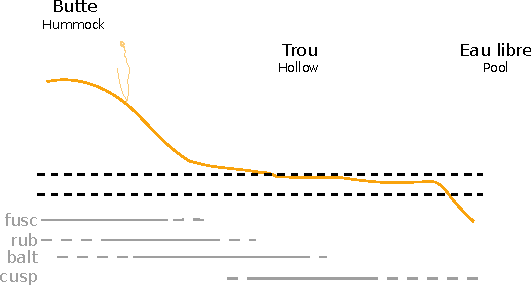
\includegraphics[width=\textwidth]{chap1/microtopo}
\caption{Micro-topographie dans les tourbières. Modifié d'après \citet{rydin2013a}}
\label{fig:microtopo}
\end{figure}

\begin{figure}
\centering
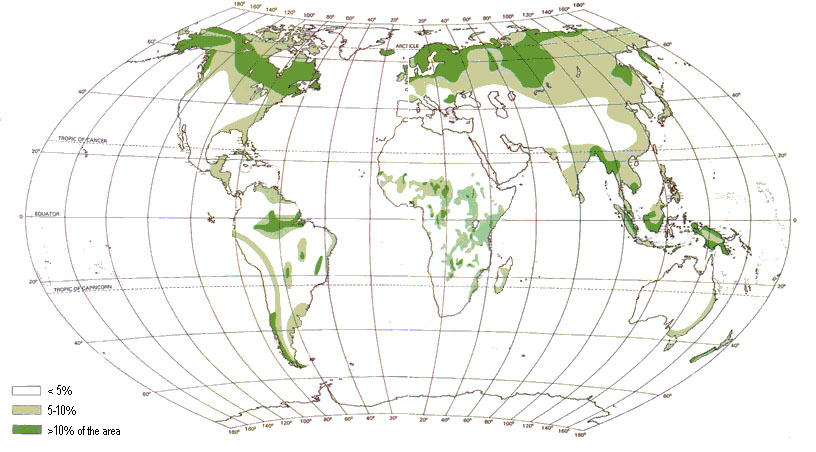
\includegraphics[width=\textwidth]{chap1/peatlandGlobalDistribution}
\caption{Global distribution of peatlands}
\label{fig:peatlandGlobalDistribution}\index{tourbières!distribution} 
\end{figure}

\subsubsection{La formation des tourbières}
\index{tourbières!formation} 
L'atterrissement\index{atterrissement} et la paludification\index{paludification} sont les deux processus principaux permettant la formation des tourbières (Figure~\ref{fig:peat_formation}).
Il s'agit pour le premier du comblement progressif d'une zone d'eau stagnante.
La paludification est la formation de tourbe directement sur un sol minéral, grâce à des conditions d'humidité importante.
Ces modes de formation ne sont pas exclusifs, une tourbière pouvant se développer, selon les endroits considérés ou le temps, via des processus différents.

\begin{figure}
\centering
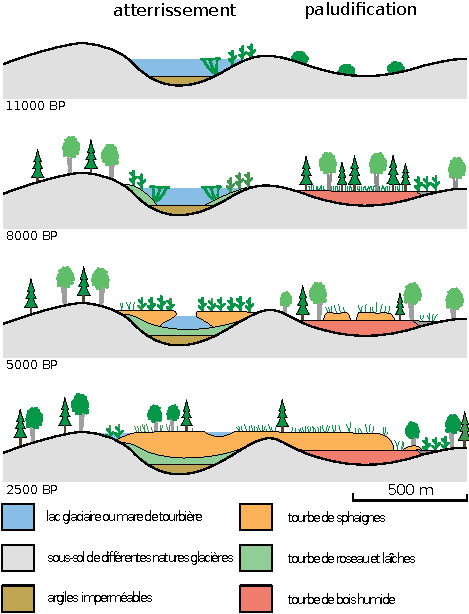
\includegraphics[width=\textwidth]{chap1/peat_formation}
\caption{Processus de formation des tourbières, à gauche l'atterrissement et à droite la paludification. modifié d'après \citet{manneville1999}}
\label{fig:peat_formation}
\end{figure}

\subsubsection{Classifications}

Différentes classifications sont utilisées pour différencier ces écosystèmes.
La plus générale et la plus utilisée dans la littérature distingue les tourbières dite haute, ou de haut marais, correspondant au \textit{bog} anglais, et les tourbières basse, ou de bas marais, correspondant au \textit{fen} anglais.

Les tourbières de haut-marais ont généralement une épaisseur de tourbe supérieure à \SI{30}{\cm} et sont alimentées principalement par les précipitations : elles sont dites ombrotrophes.
Leur surface parfois bombée (tourbières élevées ou bombées) peut également être plate ou en pente.
Cette géométrie situe une partie au moins de l'écosystème au dessus du niveau de la nappe.
Elles ont une concentration en nutriments relativement faible : elles sont oligotrophes et sont fortement acide avec des eaux de surface dont le pH est autour de 4 voire moins.

Les tourbière de bas-marais ont une épaisseur généralement supérieure à \SI{30}{\cm} avec un niveau de nappe très proche de la surface du sol.
De forme concave ou en pente elles sont généralement alimentée en eaux par des sources ou par ruissellement et sont donc dites minerotrophes.
Le pH de leur eaux de surface varient de 4 à 8.
Les végétations dominantes de ces écosystèmes peuvent être des bryophytes, des graminées ou des arbustes bas.
%De nombreux critères existent pour classer les tourbières selon leur mode de formation, leur source d'eau, leur physico-chimie.
%La terminologie utilisée concernant ces écosystèmes n'a pas toujours été cohérente, de nombreux termes ont été utilisés parfois en contradiction les uns avec les autres \cite{joosten2002}.
%Il existe différents types de tourbières, notamment on distingue des tourbières tempérées/boréales des tourbières tropicales dont le fonctionnement diffère.
%Dans la suite de ce document seule les tourbières tempérées/boréales seront décrites et étudiées.


\subsection{Tourbières et fonctions environnementales}



\subsubsection{Biodiversité dans les tourbières}

%\subsection{Les tourbières, des écosystèmes particuliers}

%\subsubsection{Biodiversité}

%Ces écosystèmes sont le siège d'une biodiversité spécifique relativement importante et rendent un certain nombre de services écologiques.
%Parmi la végétation caractéristique de ces écosystèmes, les sphaignes, des bryophytes (des mousses) sont normalement présentes en abondance.
%Les sphaignes ont quelques particularités qu'il convient de mentionner.
%Ce sont des espèces ingénieures, capable de modifier le milieu dans lequel elle vivent afin de l'adapter à leur besoin.
%Plus spécifiquement elles sont capable d'acidifier leur milieu, de capter les nutriments provenant de l'eau de pluie et de les séquestrer afin de défavoriser d'autres végétaux.
Les tourbières sont le siège d'une biodiversité importante et spécifique.
Ainsi les Sphaignes, qui sont des bryophytes, (des mousses) sont caractéristiques des écosystèmes tourbeux.
Ce sont des espèces dites ingénieures, capables de modifier l'environnement dans lequel elles vivent afin de l'adapter à leurs besoins.
Les sphaignes sont ainsi capable d'abaisser le pH, de capter des nutriments et de les séquestrer et ce même quand elles n'en ont pas besoin afin d'empêcher d'autres espèces notamment vasculaire d'en profiter.
Plus précisément, le fait que les sphaignes captent les nutriments via leur capitulum leur permet de les intercepter avant qu'ils ne soient captés par d'éventuelles racines positionnées plus bas \citep{malmer1994,svensson1995}.
Les sphaignes, comme de nombreuse mousses ont des litières relativement récalcitrantes\footnote{il est d'usage de parler de litières récalcitrantes sans plus de précision. Il s'agit en fait de litières difficilement dégradables} \citep{hobbie1996,liu2000}.
La vitesse de décomposition relative entre les différentes espèces de sphaignes est mal connue \citep{cornelissen2007}.
Des différences ont été observées entre espèces pour les parties jeunes de la plante, mais la différence est moindre pour les parties plus anciennes \citep{limpens2003}.

\subsubsection{Qualité des eaux}


%\subsubsection{Puits de carbone}
\subsubsection{Puits de carbone}
\index{carbone!stock}
Par définition les tourbières stockent ou ont stocké du carbone.
C'est cette fonction de puits de carbone qui rend l'importance de ces écosystèmes non négligeable malgré la faible surface qu'ils représentent.
Les estimations du stock de carbone présent dans les tourbières tempérées/boréales sont comprises entre 270 et \SI{455}{\giga\tonne\,C} \citep{gorham1991,turunen2002}.
Les différences entre les estimations sont liées aux incertitudes de cartographie citées précédemment auxquelles s'ajoutent des incertitudes concernant l'épaisseur et la densité moyenne de la tourbe.
Le carbone stocké dans les tourbières représente 10 à \SI{25}{\percent} du carbone présent dans les sols et entre 30 et \SI{60}{\percent} du stock de carbone atmosphérique.

\begin{table}
\centering
\caption{Estimations des stocks de C pour différents environnements}
\label{table:CCycleStocks}
\begin{tabular}{llp{7cm}}\toprule
Compartiment & Stock (en Gt de C) & référence \\ \midrule
Tourbières & 270 -- 455 & \cite{gorham1991,turunen2002} \\ 
Végétation & 450 -- 650 & \cite{Robert2003}\\ 
Sols & 1500 -- 2000 & \cite{Robert2003,Post1982,Eswaran1993}\\ 
\coo atmosphérique & 750 -- 800 & \cite{Robert2003}\\ 
Permafrost & 1700 & \\ 
\bottomrule
\end{tabular}
\end{table}

Ce stock est un héritage datant des 10 derniers milliers d'années, l'holocène, période pendant laquelle se sont formés la majorité des tourbières \plop \citep{yu2010}.
Le fonctionnement naturel de ces écosystèmes permet le stockage du C.
C'est un des services écologiques que rendent les tourbières et que l'on appelle la fonction puits de carbone.
Cette fonction est liée an niveau élevé de la nappe d'eau, qui rend l'accès à l'oxygène est plus difficile diminuant d'autant l'activité aérobie, dont la respiration des micro-organismes et des plantes.
Cela ce traduit par une dégradation relativement faible des matières organiques.
Elle est également liée à la production de litière récalcitrante par les bryophytes.

En comparaison avec un sol forestier, l'accumulation de matières organiques n'est donc pas lié à une production primaire plus forte, mais bien à une dégradation des matières produites plus faible.

Ces perturbations peuvent induire des modifications de fonctionnement, notamment l'envahissement de ces écosystèmes par une végétation vasculaire, et changer cette fonction puits.

%\subsection{Le cycle global}
%
%Au cours des temps les tourbières ont donc accumulé du carbone... stock
%La vitesse de stockage a pu varier au cours du temps mais elle est estimé à XXXX, ainsi la majorité des tourbières actuelles ont un stock qui remonte à quelques milliers d'années.
%Les estimations précise du stock de C présent dans ces écosystèmes sont délicates, à la fois car la définition de ce qu'est une tourbière que varier selon les régions, mais également car leur étendue exacte n'est pas triviale à estimer, pas davantage que leur profondeur moyenne.
%Cependant il est usuellement admis que le stock de carbone se situe entre 270 et 500 Gt de C
%Les tourbières ont donc accumulées du carbone au cours des 10 derniers milliers d'années.
%Pour ce faire il a donc fallu que davantage de carbone soit capturé que de carbone libéré par l'écosystème.



\subsection{Les tourbières et les changements globaux}
On défini les changements globaux comme l'ensemble des modifications environnementales plus ou moins rapide, ayant lieu à l'échelle mondiale, quelle que soit leur origine. Les deux contraintes développées dans cette partie sont la pressions de l'homme : contrainte anthropique, et celle du climat : contrainte climatique.
\index{changements globaux}

\subsubsection{Contrainte anthropique}
\index{tourbières!utilisation} 

L'interaction entre les Hommes et les zones humides au sens large et les tourbières en particulier remonte probablement à l'aube de l'humanité.
De grandes découvertes archéologiques ont été faites dans ces écosystèmes témoins d'époques révolues.
Des chemins de rondins néolithique aux crannogs de l'époque romaine \citep{buckland1993}.
L’utilisation de la tourbe et des tourbières a du commencer relativement tôt, mais c'est à partir du 17\textsuperscript{e} siècle que le drainage de ces écosystèmes, pour les convertir en terres agricoles, s'est intensifié.
Au 19\textsuperscript{e} siècle, l'apparition de machines permettant une récolte industrialisée de la tourbe, a développé son utilisation comme combustible.
Enfin depuis le milieu du 20\textsuperscript{e} une part importante de ces écosystèmes ont été drainé pour développer la sylviculture.
Aujourd'hui l'exploitation principale de la tourbe est liée à son utilisation comme substrat horticole \citep{lappalainen1996,chapman2003}.
Suite à ces perturbations, la surface de tourbières altérée est estimée à \SI{500000}{\square\kilo\metre} environ, principalement du fait de leur reconversion pour l'agriculture et la sylviculture (Tableau~\ref{table:tourbeUsage}).
En France, suite à leur utilisation, principalement agricole, la surface des tourbières a été par deux entre 1945 et 1998, passant de \SI{1200}{\square\kilo\meter} à \SI{600}{\square\kilo\meter} \citep{lappalainen1996,manneville1999}.

Ces écosystèmes ont donc été et sont encore perturbés par différentes activités humaines.
\begin{table}[]
\centering
\caption{Surface de tourbe utilisée selon les usages considérés (tourbières non-tropicale). Modifié d'après \citet{joosten2002}.}
\label{table:tourbeUsage}
\begin{tabular}{lll}\toprule
Utilisation & Surface (\si{\square\kilo\meter})  & proportion (\%) \\ \midrule
Agriculture & \num{250000} & \num{50} \\ 
Sylviculture & \num{150000} & \num{30}\\ 
Extraction de tourbe & \num{50000} & \num{10}\\ 
Urbanisation & \num{20000} & \num{5}\\ 
Submersion & \num{15000} & \num{3}\\ 
Pertes indirectes (érosion, ...) & \num{5000} & \num{1}\\[1ex]
Total & \num{490000} & \num{100}\\
\bottomrule
\end{tabular}
\end{table}


\subsubsection{Contrainte climatique}

Comme nous l'avons dit, le stock de C accumulé par les tourbières s'est majoritairement constitué pendant l'Holocène.
À cette époque déjà ces écosystèmes étaient influencés par le climat, et leur développement n'a pas été linéaire sur ces douze derniers milliers d'années.
Il est reconnu que le développement des tourbières est très important au début de cette période entre il y a \num{12000} et \num{8000} ans \citep{smith2004,macdonald2006,yu2009}.
Cette période coïncide avec le maximum thermique holocène (HTM), période pendant laquelle le climat était plus chaud que aujourd’hui \citep{kaufman2004}.
Ce constat peu sembler paradoxal si l'on considère que dans la littérature concernant les tourbières et le réchauffement actuel, la crainte de voir ces écosystèmes se transformer en source de C est majoritaire.
Cependant ces même auteurs qui ont montré cette relation, entre le HTM et le développement important des tourbières, ne préjugent pas de l'effet du réchauffement actuel.
Notamment \citet{jones2010} expliquent que pendant cette période de maximum thermique, existe également une saisonnalité très importante, avec des été chauds et des hivers froid, qui a dû en minimisant la respiration hivernale de ces écosystèmes, jouer un rôle important dans leur développement.

Cette forte saisonnalité n'est pas attendue lors du réchauffement actuel.
L'effet estimé dans les hautes latitudes, semble plus important pendant l'hiver et l'automne, et tendrait donc à la minimiser \citep{christensen2007}.
Les effets directs attendus du réchauffement dans les hautes latitudes à l'horizon 2100, sont une augmentation des températures de 2 à \SI{8}{\degreeCelsius} dans les zones boréales, et de 2 à \SI{6}{\degreeCelsius} dans les zone tempérées, ainsi  qu'une augmentation probable des précipitations \citep{christensen2013,frolking2011}.
De façon plus indirecte est attendue la fonte du permafrost, l'augmentation de l'intensité et de la fréquence de feux et des changements dans les compositions des communautés végétales.

%L'impact anthropique direct n'est par la seule perturbation auxquelles sont soumises les tourbières.
%D'après les modèles de prédictions du GIEC, les tourbières, comme de nombreux autres écosystèmes, vont subir un changement climatique important dans les années à venir.
%Toujours d'après le GIEC, les changements les plus rapides que ce soit en terme de précipitations ou de température sont à attendre dans les zones boréales là ou se situent la majorité des tourbières.
%De ce constat découle un certain nombre de questions concernant ces écosystèmes.
%D'abord quel effet auront les changements climatiques et avec quelle variabilité régionale ?
%Cette question n'est pas évidente (paradoxe du sol plus froid ? augmentation photosynthèse)
%Quelle sera la sensibilité des tourbières ?
%Là encore leur diversité, leur répartition géographique rend difficile la réponse à cette question.
%Enfin découlant des précédentes, qu'elle est le devenir de la fonction puits de carbone.
\begin{figure}
\centering
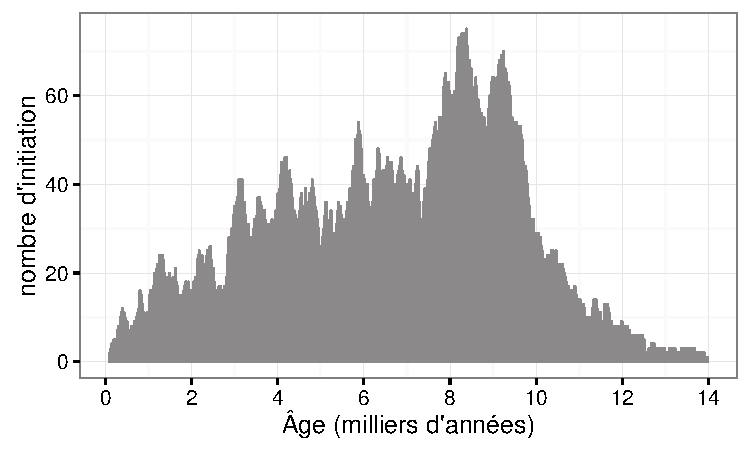
\includegraphics[width=\textwidth]{chap1/holo_peat_ini}
\caption{Nombre de tourbières nouvellement formées pendant l'holocène. Modifié d'après \citep{macdonald2006}}
\label{fig:holo_peat_ini}
\end{figure}


\begin{figure}
\centering
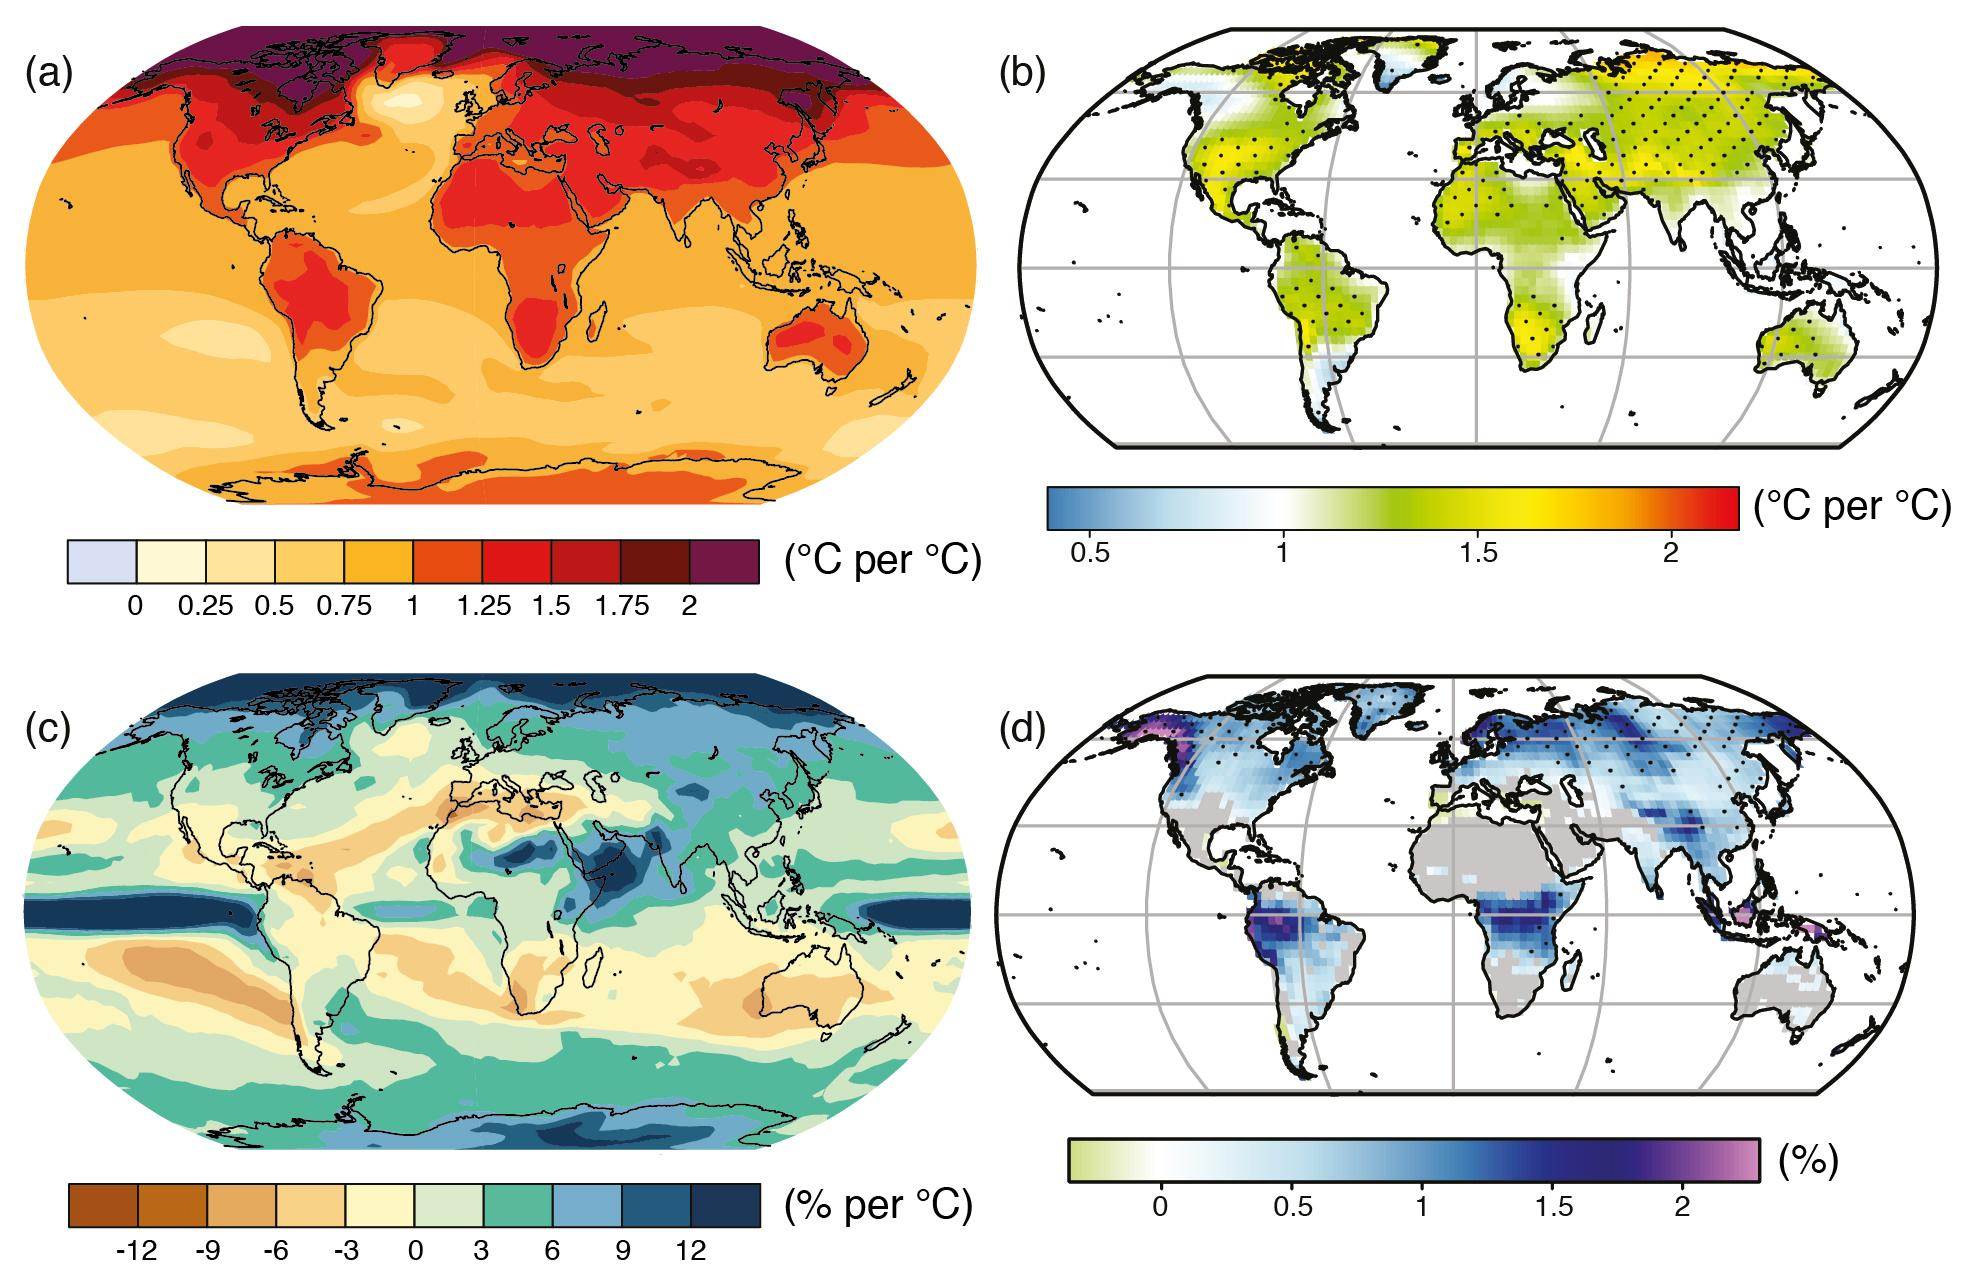
\includegraphics[width=\textwidth]{chap1/ipcc2013_RCP45}
\caption{Projection des changements à l'horizon 2100, des moyennes et extrêmes annuels (sur terre) des températures de l'air et des précipitations : (a) température de surface moyenne par \si{\degreeCelsius} de changement global moyen, (b) 90\textsuperscript{e} percentile des températures journalières maximum par \si{\degreeCelsius} de changement de température moyenne maximale, (c) précipitations moyenne (en \si{\percent} par \si{\degreeCelsius} de changement de température moyenne) et (d) fraction de jours ayant des précipitations dépassant le 95\textsuperscript{e} percentile. Sources : (a) et (c) simulations CMIP5, scénario RCP4.5, (b) et (d) adaptation d'après \citet{orlowsky2012}(\textbf{IPCC2013}).}
\label{fig:ipcc2013_T_rain}
\end{figure}

%Toutes ces perturbations posent notamment la question de la pérennité de la fonction puit de carbone de ces écosystèmes.

Les tourbières, qui ont accumulées un stock de carbone important, sont donc soumises à des contraintes fortes qu'elles soient anthropiques ou climatiques.
Afin de mieux cerner le devenir de ce carbone, l'étude de ces écosystèmes, des flux de carbone qu'ils échangent avec l'atmosphère, est une nécessité.

\index{tourbières|)}

\section{Flux de gaz à effet de serre et facteurs contrôlants}

Cette partie s'attache à décrire les GES et leurs liens avec les tourbières, les flux de carbone et des processus qui y sont liés, puis facteurs contrôlants ces flux à l'échelle des processus jusqu'aux individus et communautées (nécessaire afin de pouvoir appréhender correctement ces flux à des échelles plus large), les facteurs contrôlant à l'échelle de l'écosystème (colonne de tourbe, site complet) et enfin les bilans de carbone.


\subsection{GES et Tourbières}

Dans l'atmosphère le carbone est principalement présent dans l'atmosphère sous forme de dioxide de carbone (\coo) et de méthane (\chh).

La concentration en \coo dans l'atmosphère fluctuait avant l'ère industrielle entre 180 et \SI{290}{ppm}.
En 1750 au début de l'ère industrielle sa concentration était de \SI{280}{ppm} environ avant d'augmenter pour atteindre \SI{391}{ppm} aujourd'hui (moyenne annuelle en 2011) \citep{Ciais2014}.
Différents processus permettent d'extraire du \coo de l'atmosphère, la photosynthèse, la dissolution du \coo dans l'océan et enfin l'altération de silicate et les réactions avec le carbonate de calcium.
Ces processus s'effectuent avec des échelles de temps différentes, en conséquence après une émission de \coo, il ne reste que \SI{40}{\percent} de cette émission après \SI{100}{ans}, mais il reste toujours plus de \SI{20}{\percent} après \SI{1000}{ans} et plus de \SI{10}{\percent} après \SI{10000}{ans} \citep{joos2013,Ciais2014} (Figure~\ref{fig:co2_decroissance}).

\begin{figure}
\centering
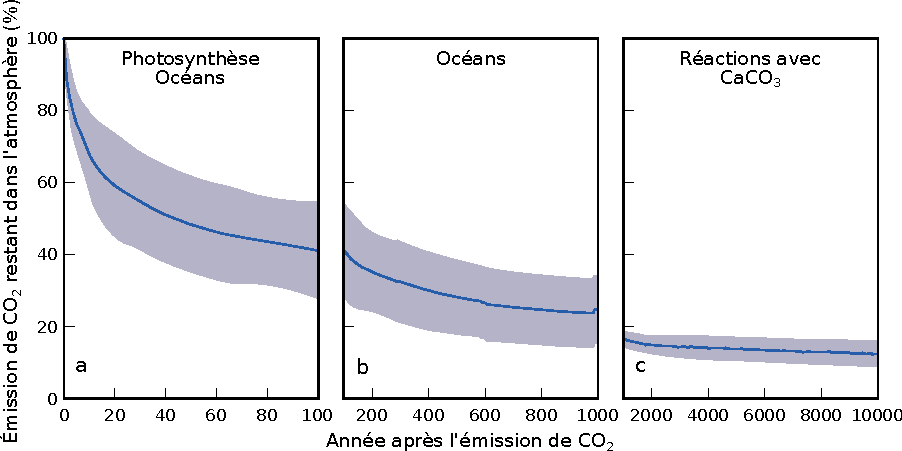
\includegraphics[width=\textwidth]{chap1/co2_decroissance}
\caption{Décroissance de la proportion de \coo de l'atmosphère suite à une émission idéalisée de \SI{100}{\peta\gram C}. les graphes (a) et (b) est une moyenne de modèles \citep{joos2013}, le graphe (c) est une moyenne d'autres modèles \citep{archer2009}. Modifié d'après \citep{Ciais2014}.}
\label{fig:co2_decroissance}
\end{figure}


La concentration en méthane de l'atmosphère est estimée à \SI{350}{ppb} il y a \SI{18000}{ans} environ lors de la dernière glaciation, à \SI{720}{ppb} en 1750, et à \SI{1800}{ppb} aujourd'hui (ou plutôt en 2011) \citep{Ciais2014}.
À l'inverse du \coo sa durée de vie dans l'atmosphère est limitée : moins de \SI{10}{ans} \citep{lelieveld1998,prather2012}.
Malgré cela son potentiel de réchauffement global\footnote{indice permettant de comparer le pouvoir de réchauffement des différents GES en donnant une équivalence par rapport au \coo. Le PRG du \coo vaut donc 1 par définition.} (PRG) est important notamment à court terme, 72 à 20 ans.
À plus long terme sont effet relativement au \coo diminue et atteint 25 à l'horizon 100 ans.
Les zones humides sont la première source naturelle de \chh atmosphérique pour avec un flux à l'échelle globale estimé entre \num{145} et \SI{285}{\tera\gram\per\year} \citep{lelieveld1998,wuebbles2002,Ciais2014} \textbf{(Tableau ?)}.
Les tourbières de l'hémisphère nord comptent pour \SI{46}{\tera\gram\per\year} \citep{gorham1991} \textbf{(pas de source plus récente ?)}.


À l'échelle globale, le stockage de C par les tourbières, prenant en compte à la fois le \coo et le \chh, est estimé à \SI{70}{\tera\gram\per\year} \citep{clymo1998}.

\subsection{Les flux entre l'atmosphère et les tourbières}

\subsubsection{De l'atmosphère à l'écosystème}

\begin{figure}
\centering
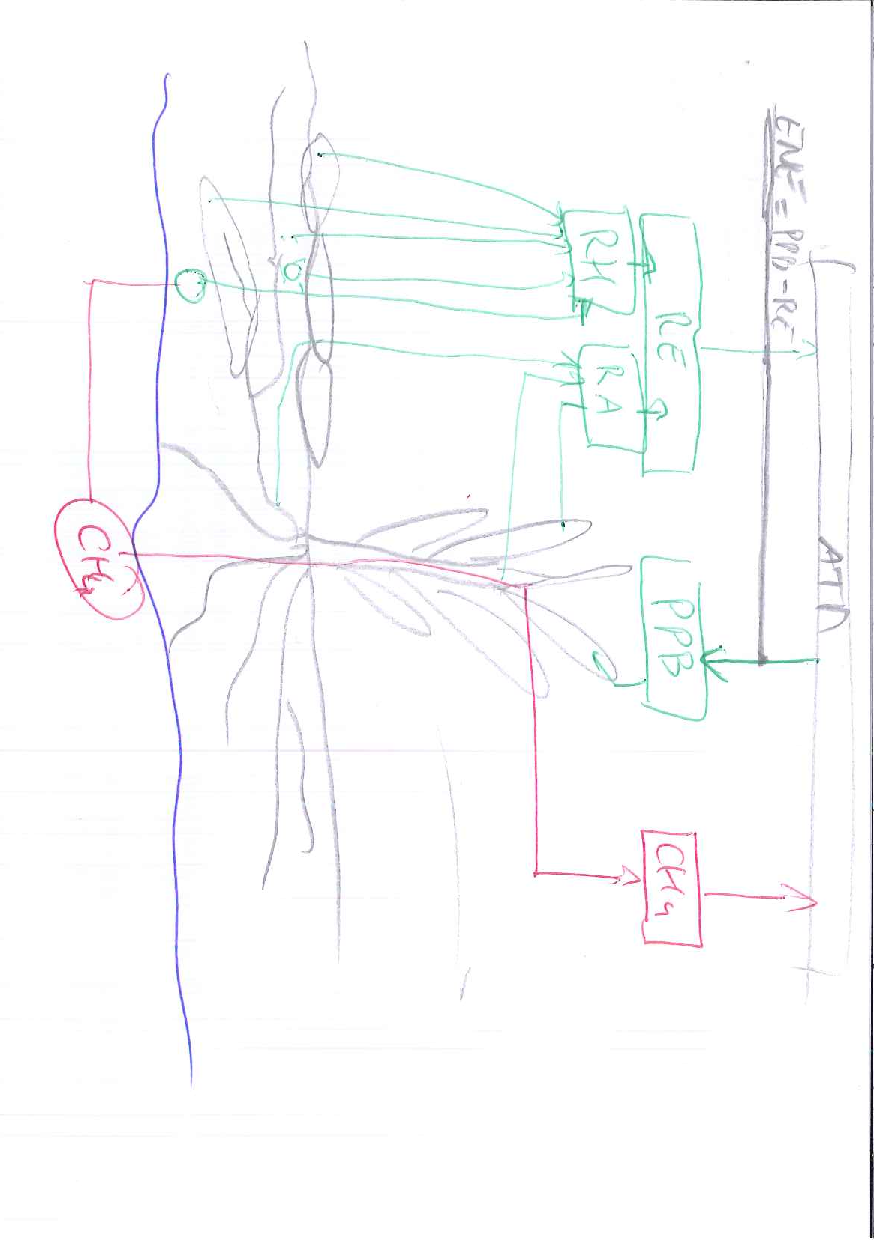
\includegraphics[height=\textwidth, angle=90]{chap1/ges_flux}
\caption{schéma des flux de carbone entre une tourbière et l'atmosphère}
\label{fig:ges_flux}
\end{figure}

Avant de stocker et de conserver du carbone, le faut le capturer.
Ce transfert du carbone de l'atmosphère à la tourbe se fait sous la forme de \coo, assimilé lors de la photosynthèse.
Principalement par les végétaux supérieurs, et éventuellement, bien que dans de moindre proportions, par des algues, des lichens ou des bactéries photosynthétiques \cite{girard2011}.
On peut écrire la réaction de photosynthèse de la façon suivante : 

$$\begin{aligned}
CO_{2} + H_{2}O + photons &\rightarrow CH_{2}O + O_{2}\\
\end{aligned} $$

Si la photosynthèse est le processus majeur d'assimilation du \coo, il existe d'autres voies métaboliques permettant la capture du \coo de l'atmosphère.\index{photosynthèse}
Par exemple les micro-organismes chemolithotrophes (\textbf{expliciter}) sont capables d'assimiler le \coo en utilisant l'énergie issue de l'oxydation de composés inorganiques, ce que l'on appelle la chimiosynthèse, mais leur importance est moindre.

On défini la \textbf{Production Primaire Brute} (PPB), \textit{Gross Primary Production}, (\textit{GPP}) en anglais
comme :

\begin{pdef}
\textsc{Production Primaire Brute (PPB)} :

Quantité de carbone extraite de l'atmosphère et transformée en matières organiques par l'écosystème principalement via la photosynthèse.
Ce flux est exprimé en quantité de carbone par unité de surface et de temps.
\end{pdef}

Les tourbières sont des écosystèmes dont la production primaire est estimée à environ \SI{500}{\gcm} \citep{francez2000}.
La strate muscinale pouvant jouer/participer/produire jusqu'à \SI{80}{\percent} de la production primaire \citep{francez2000}.
Cette production primaire n'est pas particulière élevée \plop et c'est en fait la faible décomposition des matières organiques qui permet aux tourbières de stocker du carbone.
%L'accumulation moyenne estimée dans les tourbières boréales est de \SI{30}{\gcm}. Le taux d'accumulation varie en fonction des espèces végétales présentes (\plop), le niveau d'eau (\plop), ... (??)

Il n'y a pas de flux direct de \chh de l'atmosphère vers les écosystèmes terrestres.
\SI{90}{\percent} du \chh présent dans l'atmosphère est extrait en réagissant avec des radicaux hydroxyles, cette réaction à lieu majoritairement dans la troposphère.

\subsubsection{De l'écosystème à l'atmosphère}

Les sources de carbone émises par les tourbières vers l'atmosphère sont multiples.
D'abord différents gaz peuvent être émis, notamment le \coo et le \chh, éventuellement du N\textsubscript{2}O, et certains d'entre eux peuvent être produit par différentes sources.
Au niveau cellulaire, la respiration peut être écrite sous la forme :

$$\begin{aligned}\label{eq:respi}
C_{6}H_{12}O_{6} + 6O_{2} &\rightarrow 6CO_{2} + 6H_{2}O \\
\end{aligned} $$


Le \coo est produit par différents processus, la respiration aérobie (le plus gros contributeur), les respirations anaérobies ou fermentations (e.g. du glucose, de l'acétate), ou encore l'oxydation du méthane.
Les principales sources d'émissions du \coo, sont représentées dans la figure~\ref{fig:ges_flux}.
À l'échelle macroscopique la, ou plutôt, les respirations sont généralement séparées en deux.
D'un côté la respiration végétale, que ce soit celle de feuilles, des tiges, des racines et que l'on appelle la \textbf{respiration autotrophe}.
De l'autre rassemblé sous le vocable de \textbf{respiration hétérotrophe}, la respiration de la rhizosphère, liée à l'émission d'exsudats par les racines, la décomposition des litières et des matières organiques, la respiration de la faune et l'oxydation du \chh par les organismes méthanotrophes.
L'ensemble de ces respirations est défini comme : 
\begin{pdef}
\textsc{Respiration de l'Écosystème (RE)} :

%\hfill{\textit{Gross Primary Production (GPP)}}\\
Quantité de carbone émise sous forme de \coo par l'écosystème dans l'atmosphère. 
Elle englobe la respiration autotrophe et hétérotrophe en incluant ses composantes aériennes et souterraines.
Ce flux est exprimé en quantité de carbone par unité de surface et de temps.
\end{pdef}
\index{respiration!de l'écosystème}
On distingue la respiration de l'écosystème de celle du sol en définissant la respiration du sol (RS) comme l'ensemble des respirations de la colonne de sol, à l'exclusion de la partie aérienne \citep{luo20063}.\index{respiration!du sol}
Cependant, dans la littérature la respiration du sol semble parfois être considérée comme équivalente à la respiration de l'écosystème, ou du moins cette terminologie est parfois utilisée de façon synonyme à la respiration de l'écosystème \citep{raich1992}.
Les études discriminant RS et RE montre ainsi que dans des sols tourbeux RS compte pour plus de \SI{60}{\percent} de RE \cite{lohila2003}
%
%Une autre source de \coo est l'oxydation du \chh lors de sa migration des zones anoxiques aux zones oxiques de la colonne de tourbe.
%Enfin dans les zones anaérobie, le \coo peut être produit par fermentation (respiration anaérobie).
La production de \coo est donc un signal multi-sources intégré sur l'ensemble de la colonne de tourbe. 
C'est cette multitude de processus qui rend l'estimation de ce flux difficile, en effet chacune des respirations n'aura pas la même sensibilité vis à vis de facteurs contrôlant.
%La respiration de l'écosystème (RE) est définie comme l'ensemble des respirations de la colonne de tourbe, en incluant à la fois sa partie aérienne et sa partie souterraine. \index{respiration!de l'écosystème}
%La respiration du sol (SR) est elle définie comme l'ensemble des respirations de la colonne de tourbe, en excluant la partie aérienne.\index{respiration!du sol}
%La respiration du sol comprend donc principalement les respirations issues de la rhizosphère et des communautés de micro-organisme.

%Les tourbières sont des écosystèmes dont la production primaire est estimée à environ \SI{500}{\gcm} \cite{francez2000}. 



Conséquence du niveau de nappe élevé des tourbières, le développement d'une zone anoxique importante dans la colonne de sol favorise la production de \chh.
Il est produit par des Archaea méthanogènes, des organismes anaérobies vivants sous le niveau de la nappe.
En moyenne des flux de \chh mesurés dans les tourbières s'étendent de 0 à plus \SI{0.96}{\uml}, avec généralement des flux compris entre \num{0.0048} et \SI{0.077}{\uml} \citep{blodau2002}.
Le \chh est principalement produit à partir d'acétate (CH\textsubscript{3}COOH) ou de dihydrogène (H\textsubscript{2}), ces deux composés étant dérivés de la décomposition préalable de matières organiques \citep{lai2009}.

$$\begin{aligned}
CH_{3}COOH  &\rightarrow CH_{4} + CO_{2}\\
4H_{2} + CO_{2} &\rightarrow CH_{4} + 2H_{2}O\\
\end{aligned} $$
Le \chh produit est transporté dans l'atmosphère par diffusion, ébullition ou à travers certaines plantes \citep{joabsson1999,colmer2003}.
Pendant ce transport le \chh peut être oxydé par des organismes méthanotrophes. \textbf{(Détailler dégradation \chh)}
Cette transformation produit tour à tour différents composés (méthanol, formaldéhyde, formate) aboutissant à la production de \coo \citep{whalen2005}.

$$
CH_{4} \rightarrow CH_{3}OH \rightarrow HCHO \rightarrow HCOOH \rightarrow CO_{2} \\
$$

On défini le flux de \chh comme : 
\begin{pdef}
\textsc{Flux de \chh (\fchh)} :

%\hfill{\textit{Gross Primary Production (GPP)}}\\
Quantité de carbone émise sous forme de \chh par l'écosystème dans l'atmosphère, suite au bilan des processus de création et de destruction de la molécule.
Ce flux est exprimé en quantité de carbone par unité de surface et de temps.
\end{pdef}

%Sa variabilité est donc fonction des conditions environnementales, des communautés (principalement microbiennes et végétales) impliqués 



Cette partie montre donc que si le flux de carbone de l'atmosphère à l'écosystème à pour source quasiment unique la réaction de photosynthèse des plantes, le flux de carbone de l'écosystème vers l'atmosphère est multi-source avec un nombre important de réactions de respirations et de fermentations.
La variabilité du premier vient donc majoritairement de la composition des communautés végétales et de leurs sensibilités aux conditions environnementales.
Celle du second est multiple, liée à la diversité des réactions et communautés végétales ou animales impliquées, de leur sensibilité aux conditions environnementales.

\subsection{Les facteurs majeurs contrôlant les flux}

Dans cette partie seront décrit les facteurs qui contrôlent les flux de carbone en commençant à une échelle relativement fine pour atteindre celle de l'écosystème qui nous intéresse plus particulièrement.
Cette échelle inclue la colonne de tourbe, le mésocosme, en tant que partie d'un ensemble plus vaste, en tant que sous-écosystème. 
Elle inclue forcément l'écosystème dans son sens général, regroupant les écosystèmes tourbeux mais également l'écosystème au sens plus spécifique de l'entité étudiée.

Les facteurs majeurs qui contrôlent ces flux de carbone sont globalement connus.
Comme bon nombre de réactions biochimiques les vitesses de réaction des processus décrit précédemment sont fonction de la température.
Cette relation est connue depuis longtemps.
Elle a été mise en évidence par un chimiste suédois en 1889 : Svante August Arrhenius sur la base de travaux réalisés par un autre chimiste, néerlandais, Jacobus Henricus Van't Hoff.
Le niveau de la nappe, interface entre un monde oxique et un monde anoxique, et la teneur en eau du sol vont également jouer sur ces flux.
La végétation également que ce soit de façon directe comme siège de la photosynthèse ou indirecte, en fournissant des nutriments de son vivant à travers les exsudats racinaires, ou à sa mort en devenant litière.


\subsubsection{la photosynthèse}
\index{production primaire brute!contrôle}

\begin{figure}
\centering
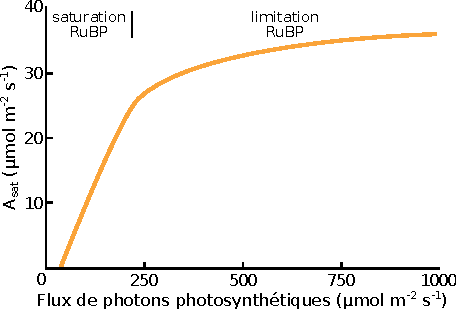
\includegraphics[width=.8\textwidth]{chap1/PAR_photo}
\caption{todo, modifié d'après \citet{long1993}}
\label{fig:PAR_photo}
\end{figure}

À l'échelle d'espèces végétales, la quantité de carbone assimilable par la photosynthèse est fonction de la quantité de lumière reçue \citep{long1993}.
La quantité de carbone assimilée augmente d'abord de façon linéaire avec le rayonnement, avant d'être limitée par la régénération d'une enzyme, la Rubisco\footnote{ribulose-1,5-bisphosphate carboxylase/oxygénase}, nécessaire à la fixation du \coo (Figure~\ref{fig:PAR_photo}).
Les limitations de l'assimilation, que ce soit la pente initiale de la partie linéaire, ou l'assimilation maximale, varient de façon importante en fonction de l'espèce considérée \citep{wullschleger1993}.
La régénération de la Rubisco, qui limite la photosynthèse, est contrainte par la capacité de transport des électrons.
La vitesse de ce transport est liée à la température et est traditionnellement décrit par une équation d'arrhenius modifiée, relativement complexe, ou par une équation simplifiée \citep{farquhar1980,june2004}.
À cette échelle le niveau de l'eau va également influer sur le développement de la végétation en facilitant plus ou moins leur accès à l'eau.
\citet{wagner1984} montent par exemple que deux espèces de sphaignes ont des tolérances différentes à la dessiccation : celle vivant dans les gouilles étant plus résistante à celle vivant sur les buttes.
Dans des conditions expérimentales différentes, lors de ré-végétalisation de deux tourbières, \cite{robroek2009} montre que différentes espèces de sphaignes vont se développer de façon optimale à différents niveaux de nappe selon leurs affinités.
Cette variabilité entre espèces d'une même famille est également mise en évidence par leur variabilité en terme de productivité primaire (Figure~\ref{fig:prod_sphagnum}).

Cette variabilité de la productivité primaire est également visible entre les communautés végétales.
Les bryophytes n'ont pas la même productivité primaire que les graminées ou que les arbustes.
En plus de ces différences entre groupes de végétaux, il existe également des différences de productivité pour un même groupe selon le type de tourbière \citetext{\citealp{moore2002} dans \citealp{rydin2013b}}.
\citet{weltzin2000} montrent par exemple que dans les tourbières de haut-marais, les sphaignes et les arbustes ont une productivité importante, les herbacées et graminées ont une productivité beaucoup plus faible.
À l'inverse ce sont les herbes et les graminées qui ont la plus forte productivité dans les tourbières de bas-marais pauvres.
devant les sphaignes puis les arbustes.
Toujour à cette échelle, le niveau de la nappe contraint la teneur en eau du sol et la hauteur de la frange capillaire.
Cette dernière atteint généralement la surface tant que le niveau de la nappe ne descend pas en dessous de \num{30} à \SI{40}{\centi\metre} \citep{laiho2006}.
La hauteur du niveau d'eau va influer sur le bien-être des différentes communautés végétales.
Un niveau d'eau important risque de diminuer l'accès de la végétation vasculaire à l'oxygène par leur racines et aux substrats tandis qu'il sera propice au développement de sphaignes.
À l'inverse un niveau d'eau faible risque de faciliter le développement de certains végétaux vasculaires au détriment des bryophytes \plop.
Cette compétition entre espèces va déterminer, à long terme, l'évolution des communautés et donc jouer sur la PPB.
Sur cet aspect \citet{gornall2011} montre que les effets des mousses sur les plantes vasculaires sont en partie positif et en partie négatif et que leur «effet net» peu varier, notamment en fonction de l'épaisseur de la strate muscinale.
La composition des communautés végétales va donc influer sur le potentiel photosynthétique de l'écosystème.
Ce potentiel qui peut varier selon le végétal considéré et les conditions environnementales dans lesquelles il se trouve \citep{moore2002}.

\begin{figure}
\centering
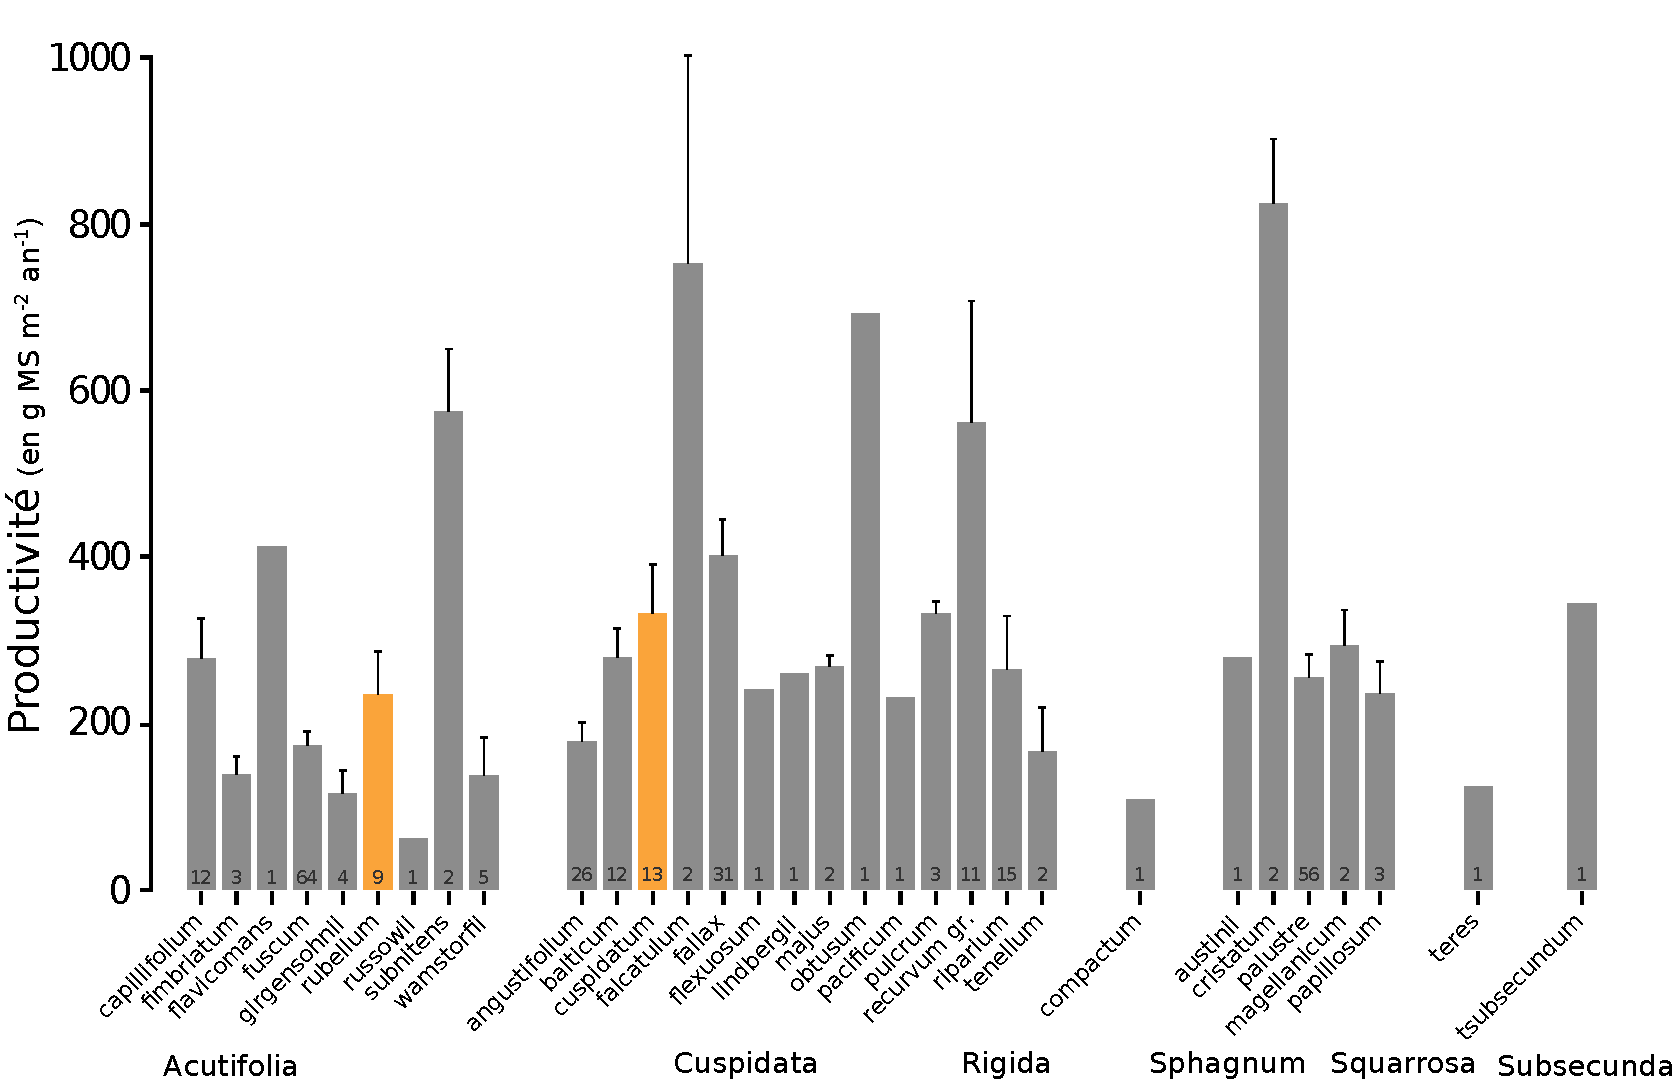
\includegraphics[width=\textwidth]{chap1/prod_sphagnum}
\caption{Productivités moyennes des espèces de sphaignes en \si{\gram\per\square\metre\per\year}. Les barres d'erreurs représentent l'erreur standard. Le nombre d'observation est indiqué par les nombres à l'intérieur des barres. Les espèces en orange sont celles rencontrées sur le site d'étude. modifié d'après \citet{gunnarsson2005}}
\label{fig:prod_sphagnum}
\end{figure}

À l'échelle de l'écosystème et sur le terrain, ces facteurs, la température, la végétation, le niveau de l'eau, covarient et rend la discrimination de leurs effets respectifs difficile.
L'effet, sur la PPB, d'une variation de température peut selon l'échelle de temps considérée, jouer sur le niveau de nappe et la végétation.
Distinguer ces facteurs n'est pas anodin, la majorité des études réalisées sur le terrain montrent les effets de variation de la température et du niveau de la nappe simultanément.
\citet{cai2010} ont par exemple montrés que des conditions plus chaudes et sèches pouvaient augmenter la PPB.
L'effet du niveau de la nappe peut varier selon le contexte : Dans une étude des effets à long terme de variation du niveau de la nappe, \citet{ballantyne2014} montrent qu'une baisse du niveau de la nappe entraîne une augmentation de la PPB en facilitant l'accès des plantes vasculaire à l'oxygène et aux nutriments.
Paradoxalement, la hausse d'un niveau de nappe, initialement bas et entraînant un stress hydrique important, conduira également à une augmentation de la PPB \citep{strack2013}.
Ces effets sont variables selon les communautés végétales et le contexte dans lequel elles se trouvent.
Pour un gradient de niveau de nappe qui augmente dans une tourbière de haut-marais, \citet{weltzin2000} montent une diminution de la productivité des arbustes, tandis que celle des graminées n'est pas affectée.
À l'inverse, pour un gradient similaire dans une tourbière de bas-marais, la productivité des arbustes n'est pas affectés tandis que celle des graminées augmente.
Un opposition similaire est également relevé concernant les graminées soumises à un traitement infra-rouge afin de les réchauffer.
Ces dernières voient leur productivité diminuer dans la tourbière de haut-marais et augmenter dans la tourbière de bas-marais.
\citet{munir2015} isolent également l'effet de la température en utilisant des OTC (\textit{Open Top Chamber}).
Ces dispositifs, ressemblent à des serres ouvertes et permettent de réchauffer une zone de la tourbière.
Ils montrent que dans les zones sans manipulation du niveau de la nappe, le réchauffement des OTC, augmente la PPB.

\subsubsection{La RE}
\index{respiration!de l'écosystème!contrôle}

La respiration, au sens de la réaction biochimique telle que  décrite par l'équation~\ref{eq:respi} est catalysée par la température.
Cette réaction est limitée par la quantité de substrat et la présence d'oxygène.
Dans les tourbières la limitation en substrat n'a de sens que vis-à-vis de communautés spécifiques.
Les substrats facilement utilisable, typiquement les sucres peuvent devenir limitant \plop.
La tourbière n'est qu'un tas de substrat de plus en plus difficile à dégrader avec la profondeur, plus les substrats sont facilement utilisable plus leur utilisation est rapide est plus ils risquent de devenir limitant.
Inversement moins les substrats sont dégradables plus leur utilisation est lente et plus ils s'accumulent.
Mais l'accès à l'oxygène rendu difficile par les hauteurs élevées du niveau de la nappe est prépondérant \plop.
La qualité du substrat (la facilité qu'il aura à être dégradé) va donc jouer sur la vitesse de respiration)
Par ailleurs, la photosynthèse en libérant des substrat, les exsudats racinaires, permet influe également sur la respiration.

\textbf{Partionnement de la RE}

À l'échelle de l'écosystème de nombreuses études ont mis en évidence une corrélation positive entre la respiration et la température \citep{singh1977,raich1992,luo2006}.
Cependant la diversité cumulée des processus, communautés et des conditions environnementales qui joue sur la respiration, font qu'aucune équation ne fait réellement consensus.
Malgré tout, la majorité d'entre-elles décrivent une augmentation exponentielle de la respiration avec la température.
Ainsi dans les tourbières, des études de terrain ont montré que dans des conditions plus chaude, mais également plus sèche étant donné que ces deux conditions sont difficilement séparable sur le terrain, la RE a tendance à augmenter  \citep{aurela2007,cai2010,ward2013}.
Des études à base de mésocosmes\footnote{définition méso} prélevés sur le terrain ont également montrées la relation entre les variation de RE et celle de la température\citep{updegraff2001,weedon2013}.

Le niveau de nappe, conditionnant l'accès à l'oxygène, joue également un rôle important.
Un niveau qui diminue se traduit généralement pas une hausse de la RE que ce soit à long terme \citep{strack2006,ballantyne2014} ou à plus court terme \citep{aerts1997}.

De façon plus indirecte, le type de végétation joue sur la vitesse de décomposition des litières.
La végétation peut également stimuler la respiration des micro-organismes présent dans la rhizosphère\footnote{zone du sol impacté par les racines} via la libération d'exsudats racinaires \citep{moore2002}.

\subsubsection{l'ENE}


\index{echange net de l'ecosystem@échange net de l'écosystème!contrôle}

À l'échelle de l'écosystème et selon les méthodes employées le \coo est parfois étudié comme un seul flux, généralement appelé l'échange net de l'écosystème.

\begin{pdef}
\textsc{l'Échange Net de l'Écosystème (ENE)} :

%\hfill{\textit{Gross Primary Production (GPP)}}\\
Bilan de la quantité de \coo émise par l'écosystème, calculée comme  différence entre la Photosynthèse Primaire Brute et la Respiration de l'écosystème (ENE=PPB$-$RE).
Ce flux est exprimé en quantité de carbone par unité de surface et de temps.
\end{pdef}
Ce terme correspond, au référentiel près, au \textit{Net Ecosystem Exchange} anglais, qui prend l'atmosphère comme référence\footnote{Attention cependant, certain papiers changent cette convention} (ENE=$-$NEE) \citep{chapin2006}.

Les facteurs contrôlants l'ENE sont donc les mêmes que ceux qui contrôlent la PPB et la RE.
Cependant l'effet d'un même facteur de contrôle peut être différent vis à vis de PPB et de RE selon le contexte environnemental, que ce soit par rapport à la nature de l'effet ou son importance.
Ainsi une variation de l'ENE peut parfois est contrôlé majoritairement soit par la PPB soit par la RE soit par les deux.
Par exemple, une baisse du niveau de la nappe est souvent liée dans la littérature à une baisse de l'ENE.
Cependant certains attribuent cette baisse à une augmentation de la Respiration \citep{alm1999, ise2008} (aurela2013, oechel1993) quand d'autres l'attribuent à une diminution de la photosynthèse \citep{sonnentag2010,peichl2014}.
Enfin certain voient un effet à la fois de l'augmentation de la respiration et de la diminution de la photosynthèse \citep{strack2013}.

À noter un article particulièrement intéressant \citep{lund2012} dans lequel, dans un même site une baisse du niveau de la nappe 2 années différentes entraînera une baisse de l'ENE dans les 2 cas, mais dans l'un des cas cette baisse est contrôlée par un augmentation de la respiration et dans l'autre cas cette baisse est contrôlée par une diminution de la photosynthèse.

Également un article de \citet{ballantyne2014} qui lui ne note pas d'effet d'une baisse du niveau de la nappe sur l'ENE car l'augmentation de la respiration est compensée par une augmentation de la photosynthèse.


\subsubsection{Le \chh}

La production du \chh, par des Archaea méthanogènes principalement à partir d'H2 et d'acétate, est contrôlée par la disponibilité de ces substrats \citep{segers1998}.
L'ajout de substrats à destination des méthanogènes (acétate, glucose, éthanol) tend à augmenter les émissions de \chh \cite{coles2002}.
Le niveau de la nappe est un autre facteur contrôlant les flux de \chh.
Généralement plus le niveau est important plus la zone potentiel de production du \chh est importante et plus les émissions sont fortes \citep{pelletier2007}.
Par contre une augmentation du niveau de la nappe au dessus de la surface peut conduire à une diminution des émissions de \chh (bubier1995,sundh1995 dans lai2009)
Les flux sont d'autant plus forte en présence de végétation \citep{pelletier2007}. 
Enfin la température joue généralement un rôle important, augmentant la vitesse de production et pouvant faciliter son transport par ébullition ou via la végétation \citep{lai2009}.


Le niveau de la nappe et la température semblent être les facteurs prépondérant du contrôle des flux de méthane

Enfin certaines plantes vasculaires, adaptées aux conditions de saturations en eau, peuvent faciliter l'échange de gaz entre l'atmosphère et l'écosystème grâce à un espace intercellulaire agrandit, l'Aerenchyme.


%\subsubsection{Conventions}


%
%Si les facteurs de contrôle des flux sont relativement connus, la sensibilité de ces flux à ces facteurs ne fait pas consensus.
%Elle peut varier selon les conditions environnementales ou l'échelle de temps ou d'espace considérée.
%%Par la suite nous considérons les processus à l'échelle d'une colonne de sol ou d'un écosystème et comment ils sont estimés.
%
%La prépondérance relative des ces différents flux, va donc impacter le fonctionnement des tourbières. 
%Soit elles stockent du carbone, en accumulant des matières organiques, et donc fonctionnent comme des puits ou soit elle relâchent du carbone et fonctionnent comme des sources.

À l'échelle de l'écosystème un même facteur peut influer sur différents flux.
Un facteur peut également influer sur un flux de différentes façon.
Parmi ces facteurs, l'effet du niveau de la nappe reste difficile à prédire.
Il contrôle la proportion des zones oxiques et anoxiques de la colonne de sol et donc la proportion de \coo et de \chh produit.
Il influe également sur la végétation, que ce soit à court terme (stress hydrique), ou à long terme (changement de communautés végétales).
Le niveau de la nappe, s'il monte, peut par exemple augmenter ou diminuer la PPB, selon sa hauteur de départ et la végétation présente sur le site.
Pour un même niveau moyen, il semble également que plus la variation du niveau est importante plus les flux seront fort (lesquels \plop).
Des effets de chasse ont également été observés après simulation d’événements pluvieux.
La question du niveau de la nappe est donc primordiale et sera explorée dans le chapitre~\ref{ch:4}.


\subsection{Bilans de C à l'échelle de l'écosystème}

L'étude individuelle de tel ou tel flux avec tel ou tel facteur contrôlant est nécessaire afin de comprendre ce qu'il se passe au niveau des processus.
Il est tout aussi nécessaire d'arriver à intégrer l'ensemble de la complexité naturelle.
C'est l'intérêt d'établir des bilans de carbone.

Le calcul d'un bilan de carbone à l'échelle d'un écosystème permet de déterminer si l'équilibre (où le déséquilibre) des flux tend à stocker du carbone, le système fonctionnant alors comme un puits, ou à libérer du carbone, le système fonctionnant alors comme une source.
Il existe différentes façon de réaliser le bilan de carbone d'une tourbière que l'on peut séparer en deux approches principales.
La première approche consiste à utiliser l'archive tourbeuse pour estimer des vitesses d'accumulation de la tourbe.
Cette méthode permet d'étudier la fonction puits sur des temps long (derniers millénaires) et de lier d'éventuels changements dans les vitesses d'accumulation à des facteurs environnementaux.
La seconde approche se base d'avantage sur des mesures actuelles des différents flux afin d'étudier, sur des temps forcément plus court, l'évolution de la prépondérance puits/source d'un écosystème.
Les deux approches sont donc complémentaires.


\subsubsection{Conventions}
%\begin{pdef}
%\textsc{Conventions} :

Dans ce document les flux (RE, PPB et \fchh) sont exprimés en valeur absolue afin de faciliter l'étude de leurs variations.
Les bilans seront établis en prenant l'écosystème comme référence, le carbone entrant dans l'écosystème est compté positivement et le carbone sortant négativement.
Les flux RE et \fchh seront comptés négativement et la PPB positivement.
Par la suite l'abréviation PPB et le mot photosynthèse seront employés de façon inter-changeable de même que RE et respiration et se rapportera à ces flux tels que définis dans les encadrés précédents, sauf mention contraire.
%\end{pdef}

\subsubsection{Estimation des bilans de carbone passé}

long-term apparent rate of carbon accumulation (LORCA) 
datations + dry bulk density + carbon content
(Tableau~\ref{table:lorca})

\begin{table}
\centering
\caption{Vitesse apparente d'accumulation du carbon à long terme en \si{\gcms}}
\label{table:lorca}
\begin{tabular}{llp{7cm}}\toprule
min -- max & moyenne & référence \\ \midrule
20 -- 140  & ? & Mitra2005 \\ %Xing
? & 18.6 &  Yu2009\\  %Xing
 & 17.2 & Gorham2012 \\  %Xing
 & 20 & Jones2010\\  %Xing
 & 16.2 & Borren2004\\  %Xing
 & 18.5 & Packalen2014\\ %Xing
 & 19.4 & Vitt2000\\ %Roulet2007
 & 19 & Turunen2004\\ %Roulet2007 (ombrotrophic bog)
5.74 -- 129.31 & 33.66 & Xing2015\\
\bottomrule
%CAR : 18.6 turunen2002 in Roulet2007
\end{tabular}
\end{table}
\textbf{tableau LORCA ajouter colonne contexte (exple: 7 tourbières ombrotrophes)}

\subsubsection{Estimation des bilans de carbone contemporain}

Dans cette approche on estime les flux actuels de carbone entrant et sortant de l'écosystème afin de déterminer un bilan.
Un certain nombre de flux de carbone sont présent au sein des écosystèmes terrestre (équation~\eqref{bdc})

\begin{equation}
BCNE=\frac{dC}{dt}=\overbrace{PPB - Re}^{ENE}  - F_{COD} - F_{COP} - F_{CH_{4}} \textcolor{gray}{- F_{CID} - F_{COV} - F_{CO}}
\label{bdc}
\end{equation}

\begin{itemize}
\item ENE : Échange Net de l'Écosystème
\item PPB : Production Primaire Brute
\item Re : Respiration de l'Écosystème
\vspace*{.2cm}
\item F$_{COP}$ : Flux de Carbone Organique Dissous
\item F$_{COP}$ : Flux de Carbone Organique Particulaire
\item F$_{CH_{4}}$ : Flux de Méthane
\vspace*{.2cm}
\item \textcolor{gray}{F$_{CID}$ : Flux de Carbone Inorganique Dissous}
\item \textcolor{gray}{F$_{COV}$ : Flux de Composés Organique Volatils}
\item \textcolor{gray}{F$_{CO}$ : Flux de Monoxyde de Carbone}
\end{itemize}

Les bilans les plus complets réalisées sur les tourbières comprennent la partie gazeuse, dissoute...

Dans les tourbières, les flux de \coo sont généralement les plus importants \plop, puis les flux de \chh et/ou de COD et enfin les flux de COP.

Pour estimer ces flux différentes techniques existent, notamment l'eddy covariance et les méthodes de chambre pour les flux de gaz.

D'autres méthodes, moins souvent utilisées, existent comme l'utilisation du ratio C:N (Kirk2015)

\subsection{Méthodologies, mesures et estimation des flux}

\subsubsection{Mesure des flux de gaz}

De nombreuses techniques permettent de mesurer des flux de gaz, avec en premier lieu les méthodes de chambres.


Les chambres peuvent être ouvertes, c'est à dire que la mesure se fait lorsque le gaz à l'intérieur de la chambre à l'équilibre avec celui à l'extérieur, ou fermées, dans ce cas le gaz à l'intérieur de la chambre n'est pas à l'équilibre avec celui à l'extérieur.
Elles peuvent également être dynamique, lorsqu'un système de pompe, permettant notamment de transporter le gaz jusqu'à l'analyseur, est présent.
Ou statique si le système est sans flux artificiel.

Trois grandes techniques de chambre existent.
D'abord les chambres \textbf{dynamiques ouvertes} qui se basent sur un état d'équilibre et mesurent une différence de concentration d'un gaz dont une partie passe par la chambre et l'autre non. 
Cette méthode nécessite un système de pompe et donc le passage d'un flux.
Ensuite les chambres \textbf{dynamiques fermées} qui mesurent l'évolution de la concentration du gaz au sein de la chambre à l'aide d'un système de pompe permettant l'envoi du gaz dans un analyseur externe.
Enfin les chambres \textbf{statiques fermées} qui mesurent également l'évolution de la concentration du gaz au sein de la chambre sans qu'un système de pompe ne soit présent.
Dans ce cas soit l'analyseur est présent dans la chambre, soit des prélèvements sont fait à intervalles réguliers puis analysés par la suite en chromatographie gazeuse.

Il faut noter que les dénominations anglaises de ces méthodes doit faire l'objet d'une attention particulière.
\textit{Closed chamber} par exemple est parfois utilisé pour se référer à l'état ou non d'équilibre, comme défini dans ce document, mais parfois également pour désigner les méthodes de chambre sans système de flux ce qui peut prêter à confusion \cite{pumpanen2004}.
Souvent utilisées les dénominations \textit{open}/\textit{closed} et \textit{dynamic}/\textit{static} sont décrites dans \cite{luo2006161}, une autre convention peut être rencontrée : \textit{flow-through}/\textit{non-flow-through} et \textit{steady state}/\textit{non-steady state} \cite{livingston1995}

Ces différentes méthodes ont divers avantages et inconvénients.

Ces méthodes sont souvent utilisées car elles on un coût modeste, et sont très versatiles ce qui permet leur utilisation dans de nombreuses situations.
D'autres méthodes plus globales existent comme les méthodes d'Eddy Covariance.

Les méthodes d'Eddy Covariance se base sur...

Comparaison entre les méthodes de chambre et les méthodes d'Eddy Covariance.

\subsubsection{Estimation des flux}
Quand ils ne peuvent pas être mesurés avec une haute fréquence, que se soit à l'aide de tour Eddy-covariance ou de chambres automatiques, les flux sont estimés à partir de mesures ponctuelles.
La respiration est généralement estimée en utilisant la température que se soit celle de l'air \citep{bortoluzzi2006} ou celle du sol à différentes profondeurs : \SI{-5}{\centi\metre} \citep{gorres2014,ballantyne2014}, \SI{-10}{\centi\metre} \cite{kim1992,zhu2015}.
Le niveau de la nappe est parfois prit en compte \citep{strack2013,munir2015}, plus rarement la végétation \citep{bortoluzzi2006,karki2015}.

Il existe donc une variabilité importante dans les équations utilisées, dans la nature et le nombre des facteurs pris en compte ainsi que dans la manière dont ils sont pris en compte.

L'estimation de la PPB est indirecte car très difficile/impossible à mesurer de façon directe à l'échelle d'un écosystème.
Elle est donc déduite à partir d'autres mesures :
Celles de l'ENE pour les méthodes micro-météorologiques qui utilisent l'ENE mesurée la nuit pour estimer la RE et en déduire la PPB.
Celles de l'ENE et de la RE pour les méthodes de chambre qui le permettent, ce qui permet là encore de déduire l'ENE (grâce à l'équation~X)


\section{Objectifs du travail}
%
Dans ce contexte les objectifs de ce travail sont donc (i) de caractériser la variabilité spatio-temporelle des flux et d'établir le bilan de carbone de la tourbière de La Guette, (ii) de préciser l'effet du niveau de la nappe sur les émissions lors de cycle de dessications réhumectation.
Pour ce faire une approche axée sur l'observation et l'expérimentation a été mise en oeuvre : 
\begin{itemize}
\item Dans un premier temps, a été mis en place un suivi sur la tourbière de La Guette permettant d'évaluer les flux et d'étudier leurs variations saisonnières et spatiales sur l'ensemble de l'écosystème. Ces estimations de flux ont ensuite pu être utilisées afin d'estimer le bilan de carbone de la tourbière.
\item Dans un second temps, à travers des expérimentations en mésocosmes et sur le terrain, l'effet du niveau de la nappe sur les flux de GES a été exploré, particulièrement lors de cycle de dessiccation-réhumectation.
\item Enfin un suivi des flux à haute fréquence sur plusieurs tourbières a été réalisé afin de déterminer les éventuelles différences de sensibilité des émissions de \coo entre le jour et la nuit et de tester à cette échelle une méthode d'estimation de la RE basée sur la synchronisation entre les signaux de flux et de température.
\end{itemize}
 %Synthèse bibliographique
% CHAPITRE 2
% SUIVI VARIABILITE SPATIALE

\chapter{Sites d'études et méthodologies employées}

\minitoc

\newpage

\section{Présentation de la tourbière de La Guette}

Le site d'étude, la tourbière de La Guette, est l'un des quatre sites du service national d'observation des tourbières (SNOT).


\begin{figure}[h]
\centering
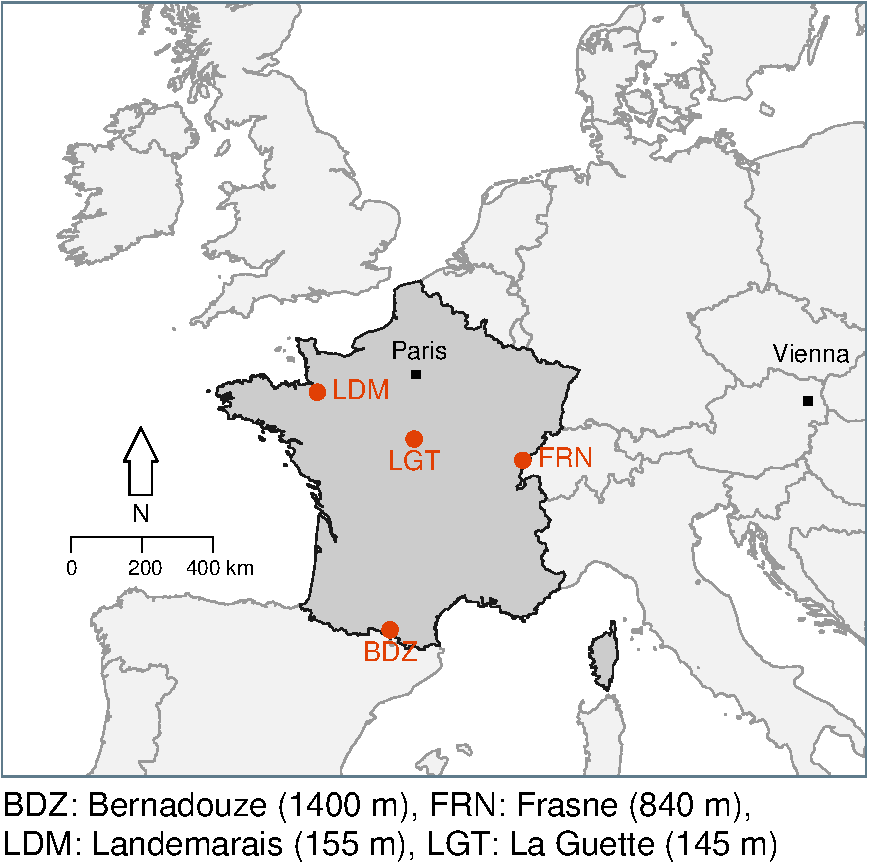
\includegraphics[width=.75\textwidth]{chap2/SNO_siteLocalisation}
\caption{Site d'études SNO}
\label{fig:carte_europe}
\end{figure}
%\subsection{La Guette}

La tourbière de La Guette est située à Neuvy-sur-Barangeon, en Sologne, (N 47\textdegree19’44”, E 2\textdegree17’04”) dans le département du Cher (Figure~\ref{fig:carte_europe}).
Le site s'étend sur une surface d'une vingtaine d'hectare avec une géométrie relativement allongée \ref{fig:carte_LG}.
Avec une conductivité généralement inférieur à 80 uS/m2 et un pH compris entre 4 et 5 elle se classe parmis les "transitionnal poor fen"
Les datations effectuées sur le site permettent de dire que les premiers dépôts tourbeux remontent à environ 5 à 6000 ans.
Le site a subi un certain nombre de perturbations au cours de son existence.
D'abord la construction d'une route, avant 1945, qui coupe l'extrémité sud de la tourbière favorisant son drainage.
Le site est également brûlé par un incendie en 1976.
En 1979 des pins noirs (\textit{Pinus nigra}) sont plantés au nord du site
Enfin 2008 le récurage du fossé de drainage bordant la route semble entraîner une augmentation significative des pertes d'eau du système.

\begin{figure}
\includegraphics[width=\textwidth]{chap2/carteGLc}
\caption{Carte de la tourbière de La Guette}
\label{fig:carte_LG}
\end{figure}

Ces perturbations, ou au moins une partie d'entre elles, ont probablement favorisé l'envahissement du site par une végétation vasculaire, notamment arborée et composée de pins (\textit{Pinus sylvestris}) et de bouleaux (\textit{Betula verrucosa} et \textit{pubescens}).
\citet{viel2015} a pu calculé, grâce à l'étude de photos aérienne, la vitesse de fermeture du site, entre 1945 et 2010, estimée à \SI{2020}{\square\metre\per\year} avant l'incendie de 1976 et à \SI{3469}{\square\metre\per\year} après.
La tourbière est également envahie de façon importante par la molinie bleue (Molinia caerula) de la famille des \textit{Poaceae} (Figure~\ref{fig:mol}).
Leur présence favorisant la dégradation des matières organiques \citep{gogo2011}.

Sont également présentes sur le site un certain nombre d'espèces caractéristiques des tourbières comme les sphaignes, principalement \textit{Sphagnum cuspidatum} et \textit{Sphagnum rubellum}, qui forment des tapis.
Un tapis de sphaignes en cours de formation est visible sur la photo~\ref{fig:sphg_erio}.
Sur cette même photo sont également visible des Linaigrettes à feuilles étroites (Eriophorum augustifolium), une plante de la famille des \textit{Cyperaceae} caractéristique des marais et des landes tourbeuses \plop.
Des bruyères sont également présentes de façon importante sur le site avec notamment \textit{Erica tetralix}, parfois appelée la Bruyère des marais, de la famille des \textit{Ericaceae} (Figure~\ref{fig:erica}).
De la même famille est présente sur le site, mais de façon moins omniprésente, la Callune (\textit{Calluna vulgaris}).
L'ensemble de ces espèces tendent à préférer les milieux riches en matières organiques et pauvres en nutriment (tela-botanica).

D'autres espèces sont présentes sur ce site notamment, \textit{Rhynchospora alba} de la famille des \textit{Cyperaceae}, \textit{Juncus bulbosus}, de la famille de \textit{Juncaceae}, et des Droséras, une plante insectivore, de la famille des \textit{Droseraceae} (\textbf{image annexe ?}). 

\begin{figure}[htbp]
    \centering
    \begin{subfigure}[b]{.98\textwidth} % "0.45" donne ici la largeur de l'image
        \centering 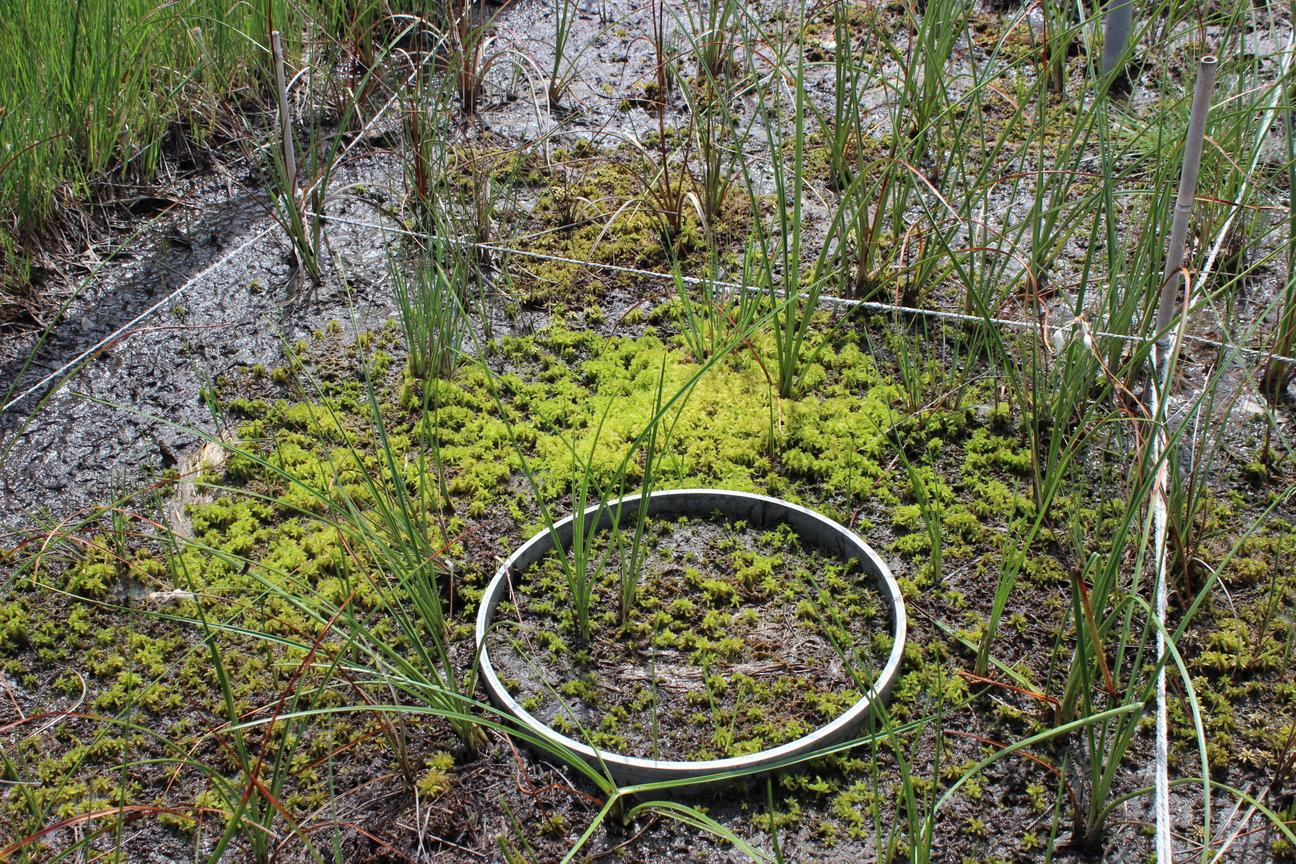
\includegraphics[trim=5cm 0cm 0cm 10cm, clip=true, width=\textwidth]{chap2/sphaigne_eriophorum_c.jpg}
        \caption{\textit{Sphagnum} -- \textit{Eriophorum augustifolium}}\label{fig:sphg_erio}
    \end{subfigure}
    
%    ~ % ce symbole ajoute un espacement horisontal entre les premières deux images
    \begin{subfigure}[b]{0.49\textwidth}
%        \centering 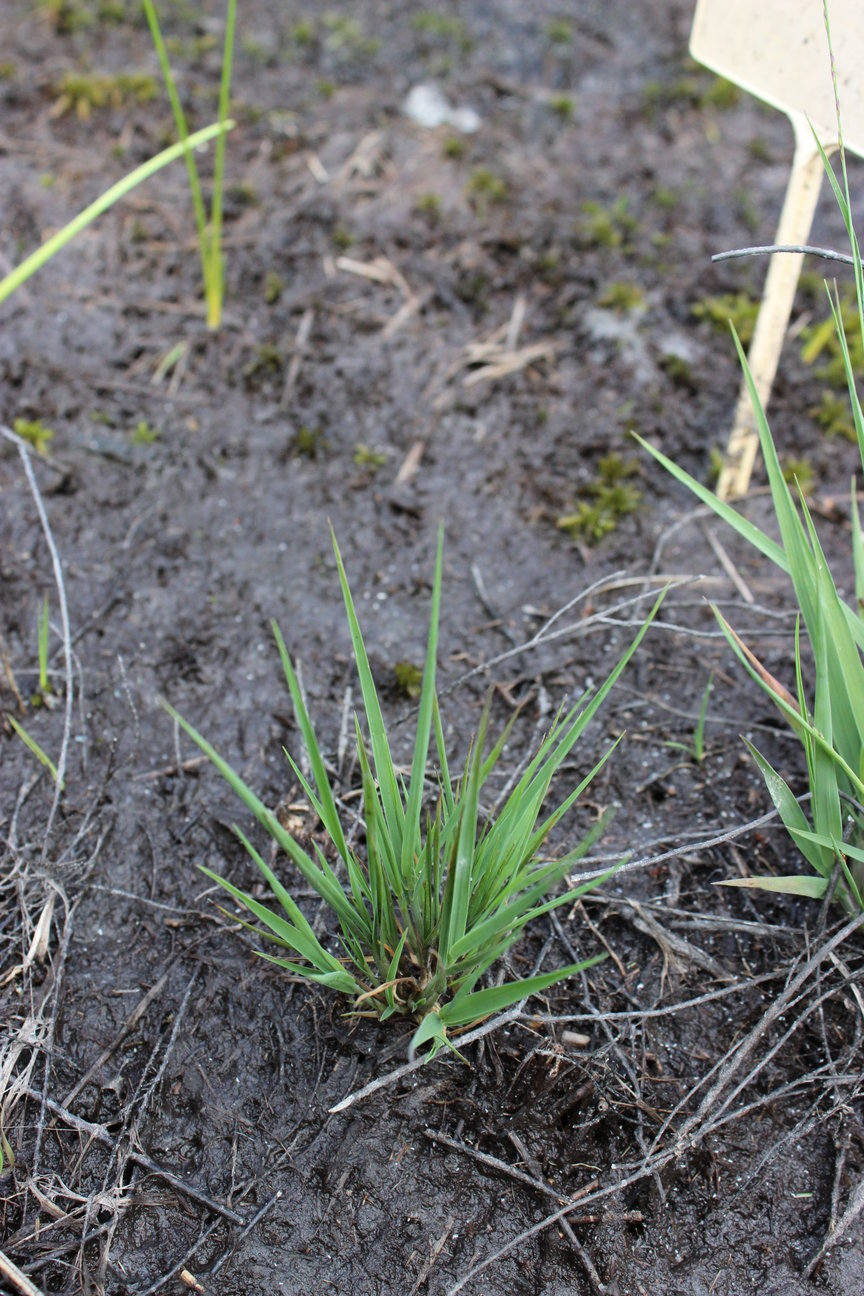
\includegraphics[trim=0cm 0cm 0cm 0cm, clip=true, width=\textwidth]{chap2/molinia_caerulea_c.jpg}
        \centering 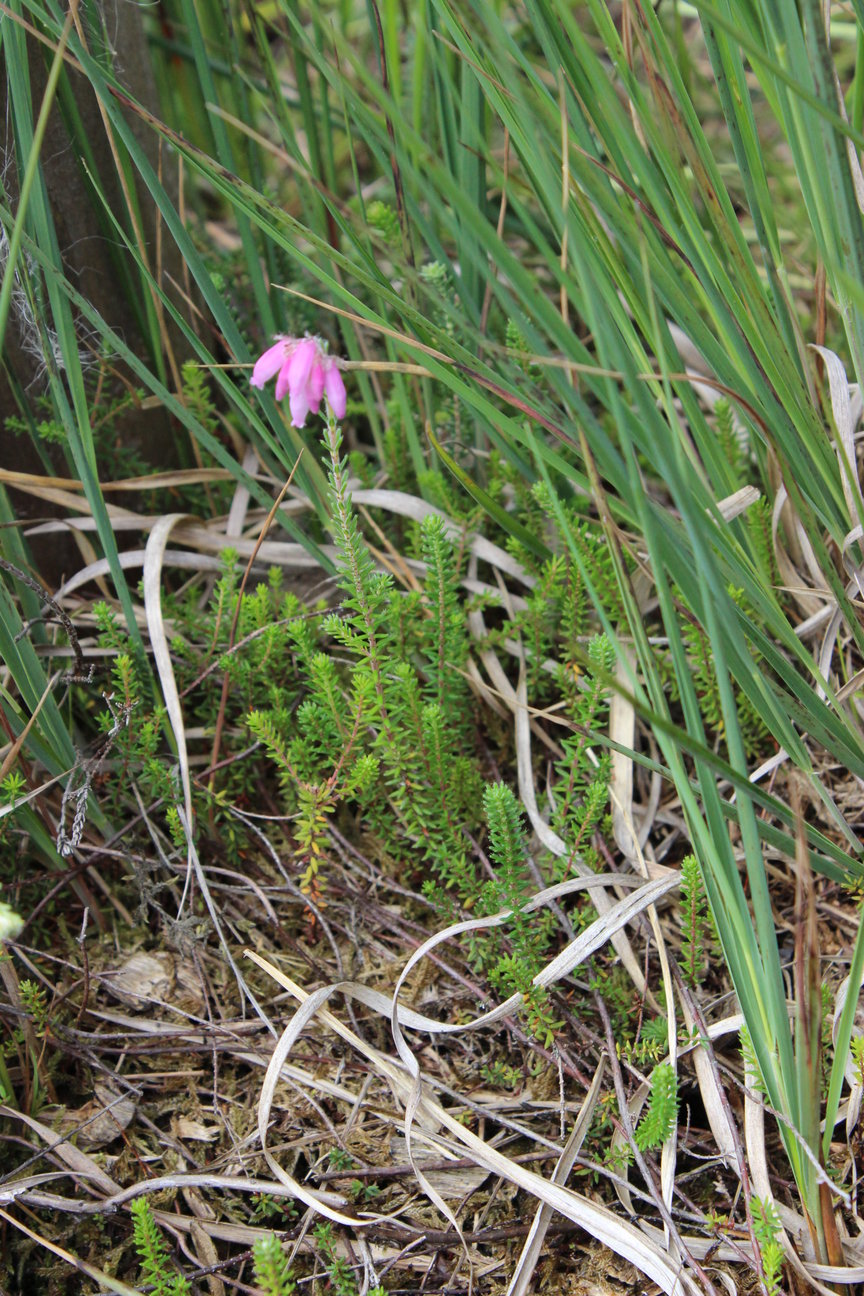
\includegraphics[trim=0cm 4cm 0cm 0cm, clip=true, width=\textwidth]{chap2/erica_tetralix_c.jpg}
        \caption{\textit{Erica tetralix} -- \textit{Molinia caerulea}}\label{fig:erica}
    \end{subfigure}
    % la ligne blanche correspond au retour à la ligne après le deuxième image
    \begin{subfigure}[b]{0.49\textwidth}
        \centering 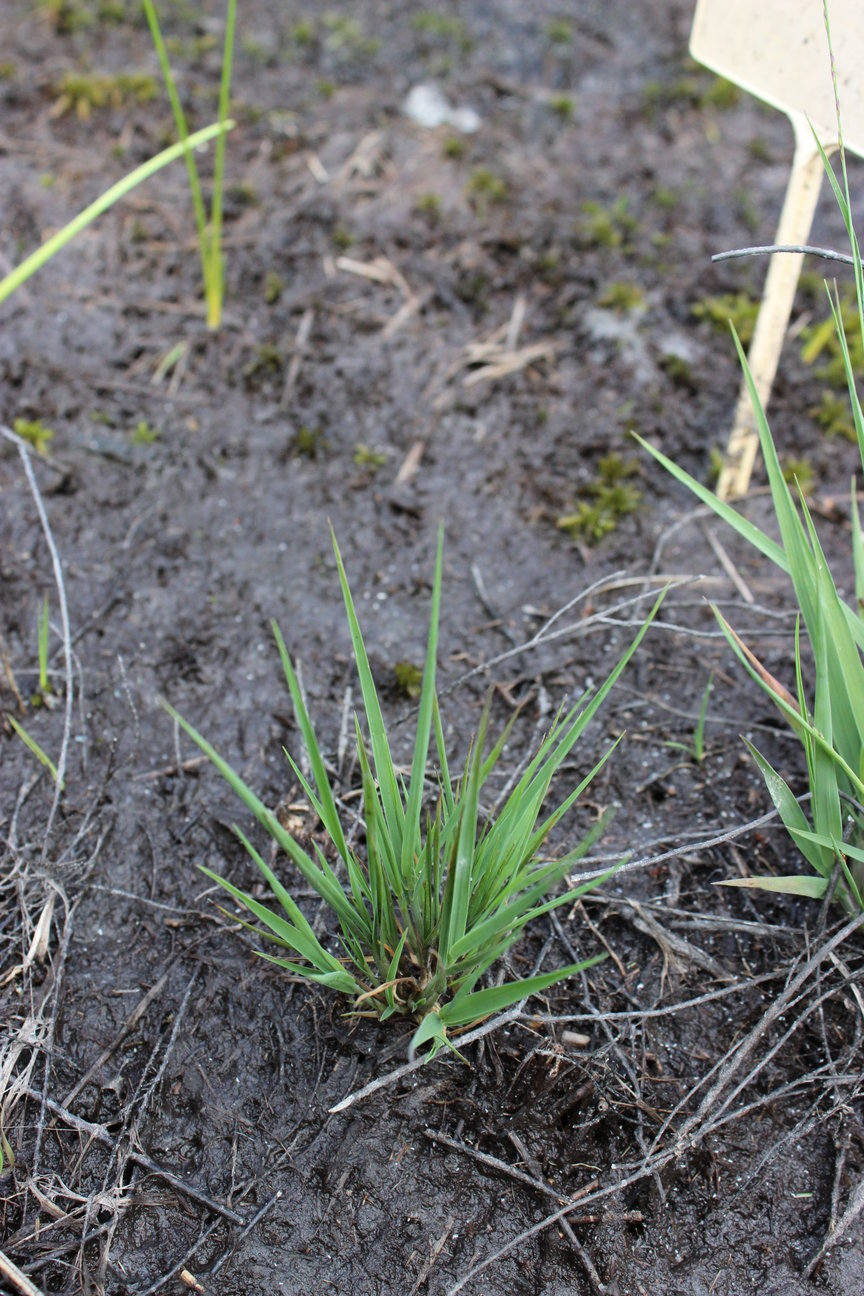
\includegraphics[trim=0cm 2cm 0cm 2cm, clip=true, width=\textwidth]{chap2/molinia_caerulea_c.jpg}
%        \centering 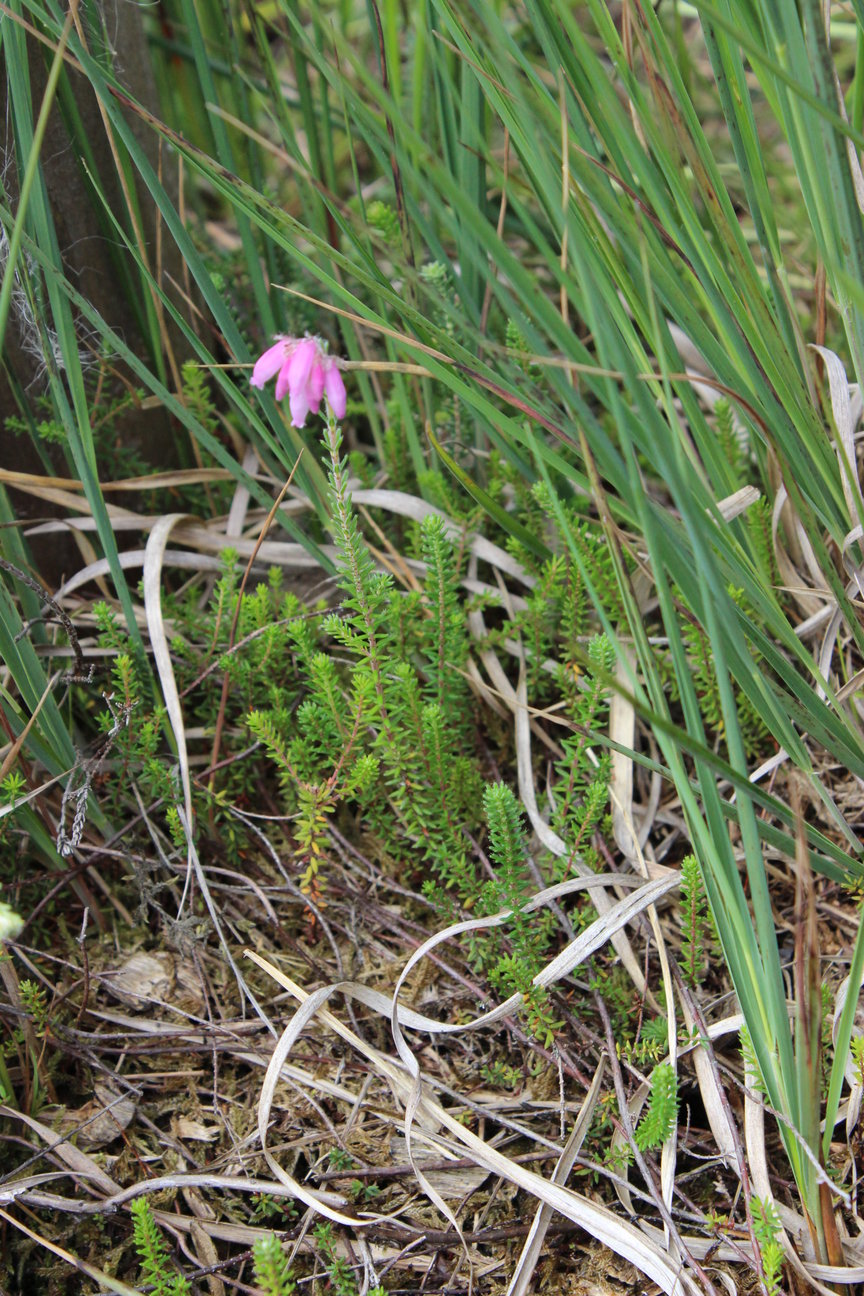
\includegraphics[trim=0cm 0cm 0cm 0cm, clip=true, width=\textwidth]{chap2/erica_tetralix_c.jpg}
        \caption{\textit{Molinia caerulea}}\label{fig:mol}
    \end{subfigure}
%    ~

%    \begin{subfigure}[b]{.8\textwidth}
%        \centering 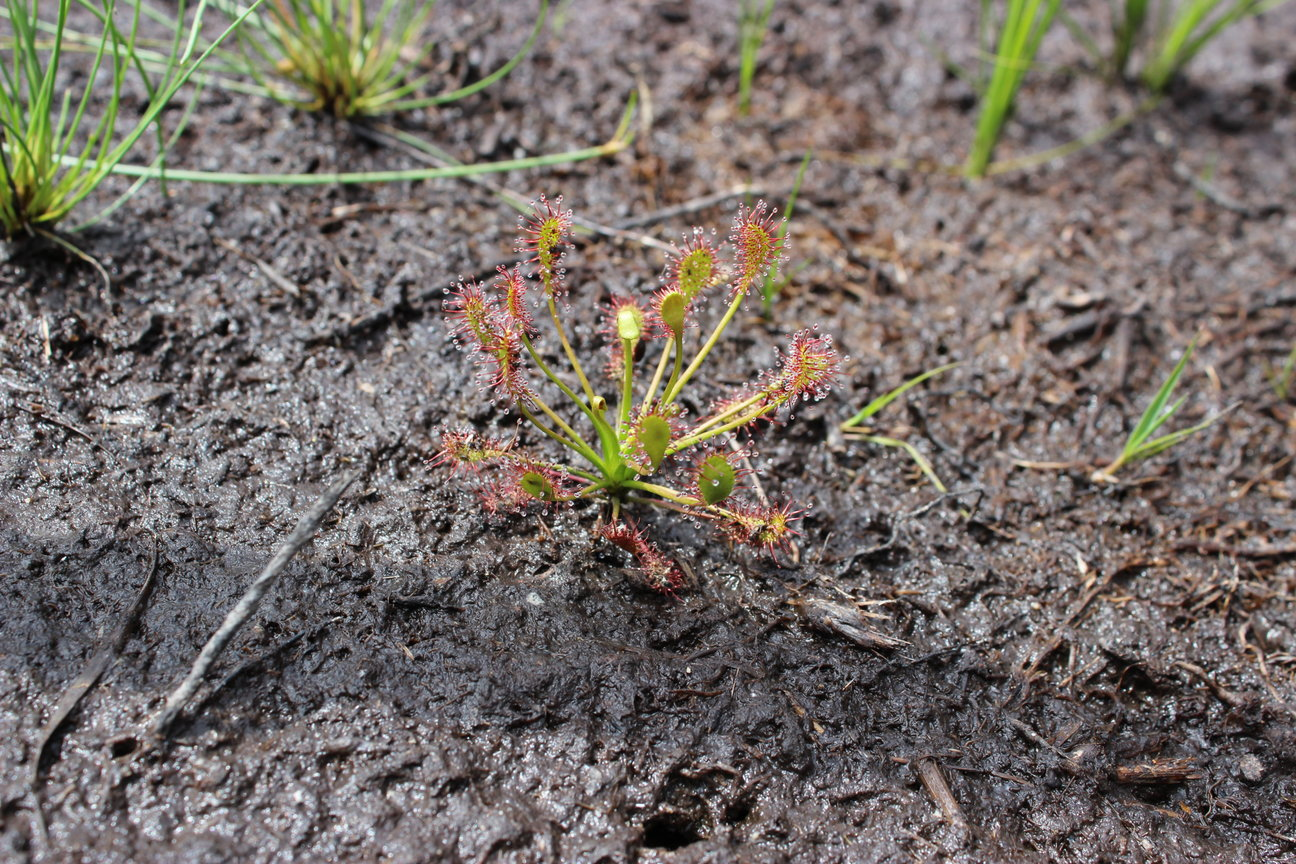
\includegraphics[trim=2.5cm 5cm 2.5cm 5cm, clip=true, width=\textwidth]{chap2/drosera_c.jpg}
%        \caption{drosera}\label{fig:dro}
%    \end{subfigure}
    \caption{Végétation présente sur le site de La Guette, et suivie lors des campagnes de mesure.}\label{fig:veg}
\end{figure}


\begin{figure}
\centering
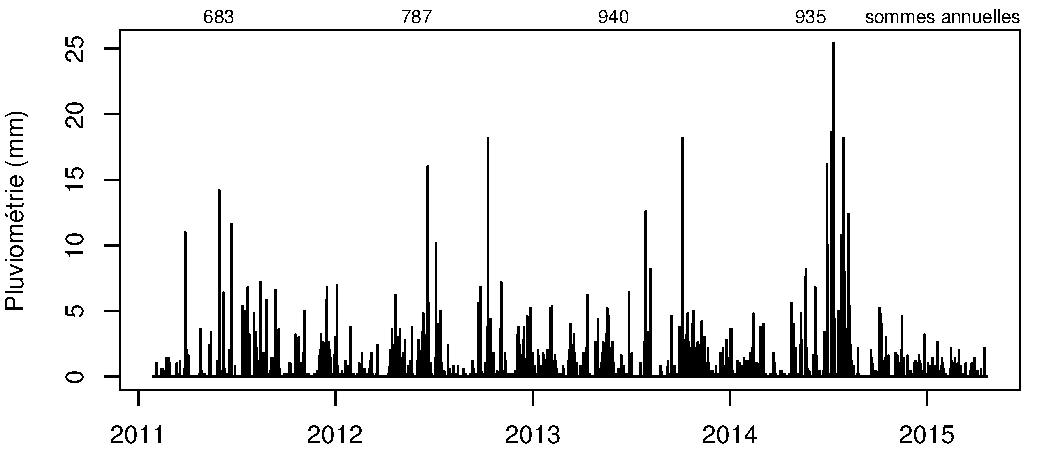
\includegraphics[width=\textwidth]{chap2/pluvio}
\caption{Évolution du niveau de la pluviométrie, en \si{\mm}, des années 2011 à 2014}
\label{fig:pluvio}
\end{figure}

\begin{figure}
\centering
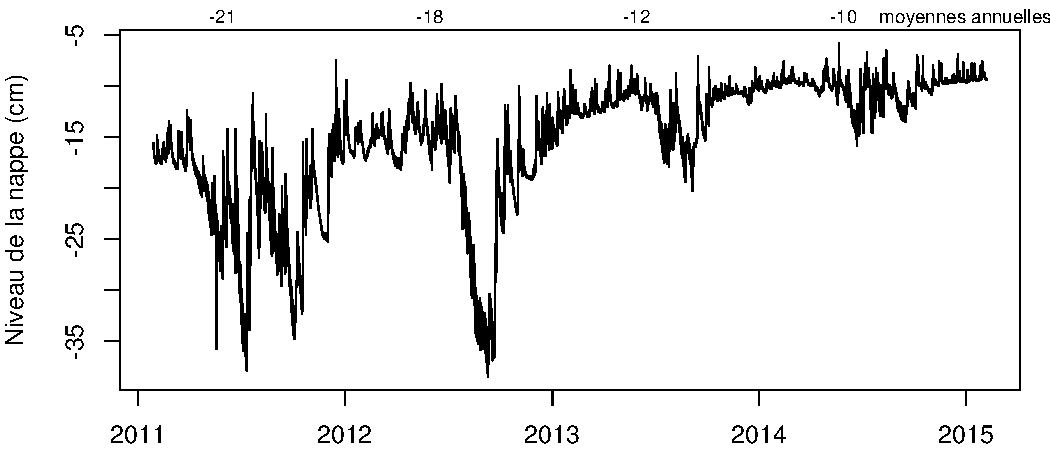
\includegraphics[width=\textwidth]{chap2/WTL}
\caption{Évolution du niveau de la nappe, en cm par rapport à la surface, des années 2011 à 2014}
\label{fig:WTL}
\end{figure}

Au cours des dernières années, les précipitations sont relativement différentes avec deux années plus sèche que la moyenne avant 2013 et deux années plus humide en 2013 et 2014 (Figure~\ref{fig:pluvio}).
On observe également cette dualité au niveau du niveau de la nappe.
Avant 2013 les étés sont marqués par des étiages important avec des baisses du niveau de nappe allant jusqu'à \SI{-60}{\cm} en 2012 (Figure~\ref{fig:WTL}).
Après 2013, les étiages sont beaucoup moins importants sur le site.



\begin{figure}
\centering
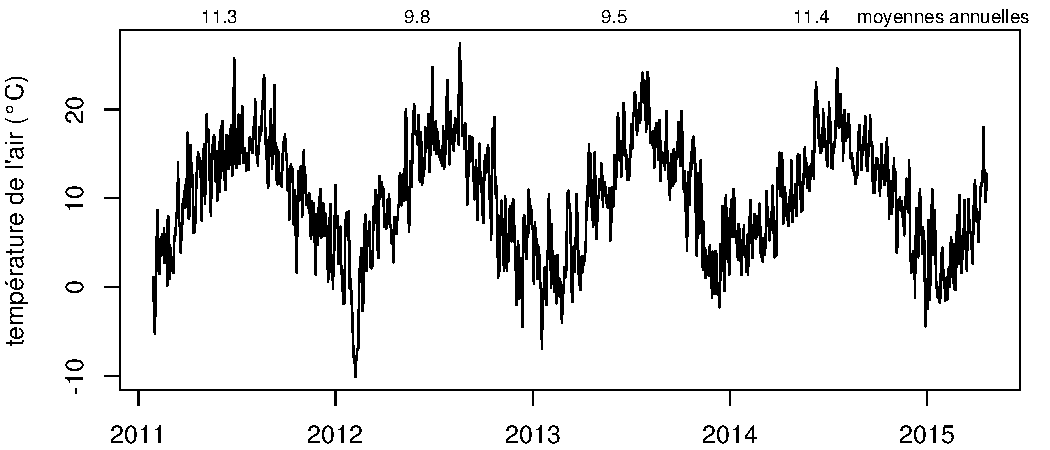
\includegraphics[width=\textwidth]{chap2/tair}
\caption{Évolution de la température de l'air (en \textdegree C) des années 2011 à 2014}
\label{fig:tair}
\end{figure}



Au sein de ses sites de nombreuses mesures ont été effectuée et notamment des mesures de flux de GES à la fois concernant le \coo et le \chh. La méthodologie étant transverse à de nombreuses expérimentations il convient de l'expliquer au préalable.

\section{Autres sites du service national d'observation}

Bien que moins étudiés, les autres sites du SNOT, Bernadouze, Frasne et Landemarais ont également fait l'objet d'un suivi ponctuel en 2013.
La tourbière de Bernadouze est situé à \SI{1400}{\metre} dans les Pyrénées, en Ariège (N 42\textdegree 48’09”, E 1\textdegree25’24”)).
Elle est relativement petite avec \SI{3.75}{\hectare} seulement.
La tourbière de Frasne est situé à \SI{840}{\metre} dans le Doubs et s'étend sur une surface de \SI{98}{\hectare}.
Enfin la tourbière de Landemarais est située en Ille-et-villaine, à \SI{154}{\metre} et sur \SI{23}{\hectare}.
les températures annuelles moyennes sur ces trois sites sont respectivement de 6, 7,5 et \SI{11}{\degreeCelsius}.
les précipitations annuelles étant de \num{1700}, \num{1400}, \SI{870}{\milli\meter}.


\section{Mesures de flux}
\label{sec:clsd_chbr_method}

\subsection{Présentation des méthodologies possibles}
De nombreuses techniques permettent de mesurer des flux de gaz, avec en premier lieu les méthodes de chambres.


Les chambres peuvent être ouvertes, c'est à dire que la mesure se fait lorsque le gaz à l'intérieur de la chambre à l'équilibre avec celui à l'extérieur, ou fermées, dans ce cas le gaz à l'intérieur de la chambre n'est pas à l'équilibre avec celui à l'extérieur.
Elles peuvent également être dynamique, lorsqu'un système de pompe, permettant notamment de transporter le gaz jusqu'à l'analyseur, est présent.
Ou statique si le système est sans flux artificiel.

Trois grandes techniques de chambre existent.
D'abord les chambres \textbf{dynamiques ouvertes} qui se basent sur un état d'équilibre et mesurent une différence de concentration d'un gaz dont une partie passe par la chambre et l'autre non. 
Cette méthode nécessite un système de pompe et donc le passage d'un flux.
Ensuite les chambres \textbf{dynamiques fermées} qui mesurent l'évolution de la concentration du gaz au sein de la chambre à l'aide d'un système de pompe permettant l'envoi du gaz dans un analyseur externe.
Enfin les chambres \textbf{statiques fermées} qui mesurent également l'évolution de la concentration du gaz au sein de la chambre sans qu'un système de pompe ne soit présent.
Dans ce cas soit l'analyseur est présent dans la chambre, soit des prélèvements sont fait à intervalles réguliers puis analysés par la suite en chromatographie gazeuse.

Il faut noter que les dénominations anglaises de ces méthodes doit faire l'objet d'une attention particulière.
\textit{Closed chamber} par exemple est parfois utilisé pour se référer à l'état ou non d'équilibre, comme défini dans ce document, mais parfois également pour désigner les méthodes de chambre sans système de flux ce qui peut prêter à confusion \cite{pumpanen2004}.
Souvent utilisées les dénominations \textit{open}/\textit{closed} et \textit{dynamic}/\textit{static} sont décrites dans \cite{luo2006161}, une autre convention peut être rencontrée : \textit{flow-through}/\textit{non-flow-through} et \textit{steady state}/\textit{non-steady state} \cite{livingston1995}

Ces différentes méthodes ont divers avantages et inconvénients.

Ces méthodes sont souvent utilisées car elles on un coût modeste, et sont très versatiles ce qui permet leur utilisation dans de nombreuses situations.
D'autres méthodes plus globales existent comme les méthodes d'Eddy Covariance.

Les méthodes d'Eddy Covariance se base sur...

Comparaison entre les méthodes de chambre et les méthodes d'Eddy Covariance.

\subsection{Les mesures de \coo}

Toutes les mesures de \coo présentées par la suite ont été faite avec les mêmes matériels et le même protocole.
Les chambres en \textbf{XXXX} ont été conçue (LPC2E) fabriquées (ISTO) au CNRS.
Ce sont des chambres transparentes, cylindrique, de \SI{30}{\centi\metre} de diamètre et \SI{30}{\centi\metre} de hauteur.
Les mesures de \coo à proprement parler ont été faite à l'aide d'une sonde Vaisala GMP 343\textregistered.
La sonde est directement inséré dans la chambre ainsi qu'une sonde Vaisala \textbf{XXXXX} mesurant d'humidité et la température dans la chambre.

Avant toute mesure, des embases sont installées sur le site.
Ce sont des cylindres de PVC d'une hauteur de \SI{15}{\centi\metre} inséré dans le sol sur 8 à \SI{10}{\centi\metre}.
La partie enterrée de ces cylindres ayant préalablement été percée d'une quarantaine de trou afin de minimiser les impacts de l'embase sur le développement racinaire et les écoulements d'eau.

La méthode mise en œuvre est celle de la chambre statique fermée.
Aucun système de pompe n'est donc utilisé, la chambre est posée sur l'embase, elle contient l'analyseur de \coo qui mesure la variation de la concentration en gaz au cours du temps.
Un ventilateur de faible puissance est également présent à l'intérieur de la chambre afin d'homogénéiser l'air présent dans la chambre.
1 à \SI{3}{\minute} sont nécessaires après la pose de la chambre afin d'éviter les effets pouvant y être liés.
Ensuite l’enregistrement est lancé, avec l'acquisition toutes les \SI{5}{\second} pendant \SI{5}{\minute} de la concentration en \coo, de la température et de l'humidité.
La mesure se déroule donc sur une période de temps relativement courte afin de minimiser le déséquilibre avec le milieu extérieur.
Dans ce but les mesures on parfois été encore raccourcie, 2 à \SI{3}{\minute} d'acquisition, si une pente claire se dégage rapidement, notamment lorsque les conditions météorologiques, chaudes et ensoleillées, laissaient supposer une différence importante vis à vis des conditions extérieures.

Généralement, deux acquisitions de \coo sont faites à la suite sur une embase.
La première, avec la chambre transparente nue, permettant l'enregistrement de l'ENE (Figure~\ref{fig:chb}-a).
La seconde avec la chambre recouverte d'une chaussette de tissu occultant, isolant la chambre de la lumière, permettant d'interrompre la photosynthèse et donc d'enregistrer les respirations (RE) (Figure~\ref{fig:chb}-b).

\begin{figure}
	\centering
	\begin{subfigure}[t]{0.5\textwidth}
		\centering
		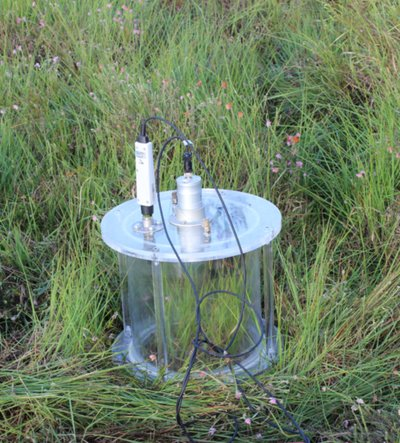
\includegraphics[width=.8\textwidth, frame]{chap2/chb_ENE}
	\end{subfigure}%
	\begin{subfigure}[t]{0.5\textwidth}
		\centering
		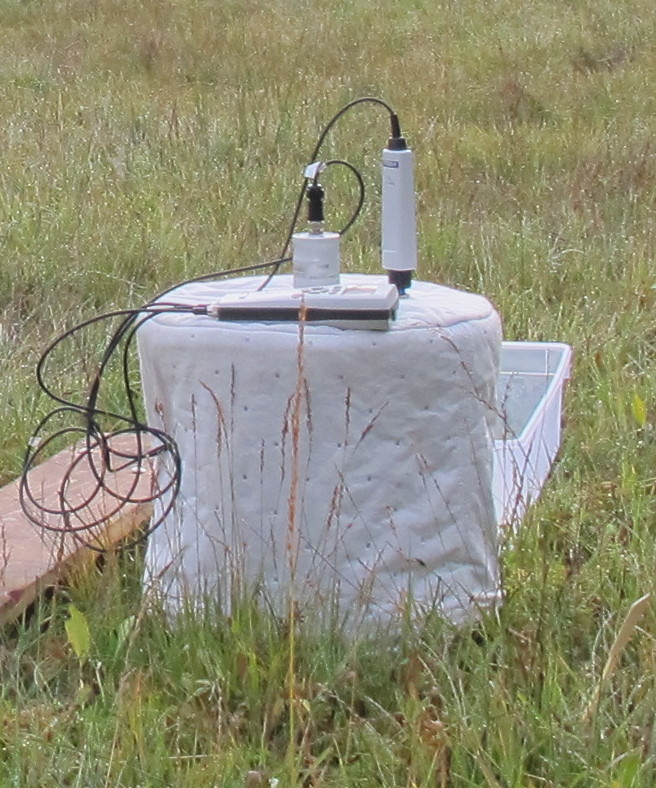
\includegraphics[width=.8\textwidth, frame]{chap2/chb_ER}
	\end{subfigure}%

	\begin{subfigure}[t]{0.5\textwidth}
		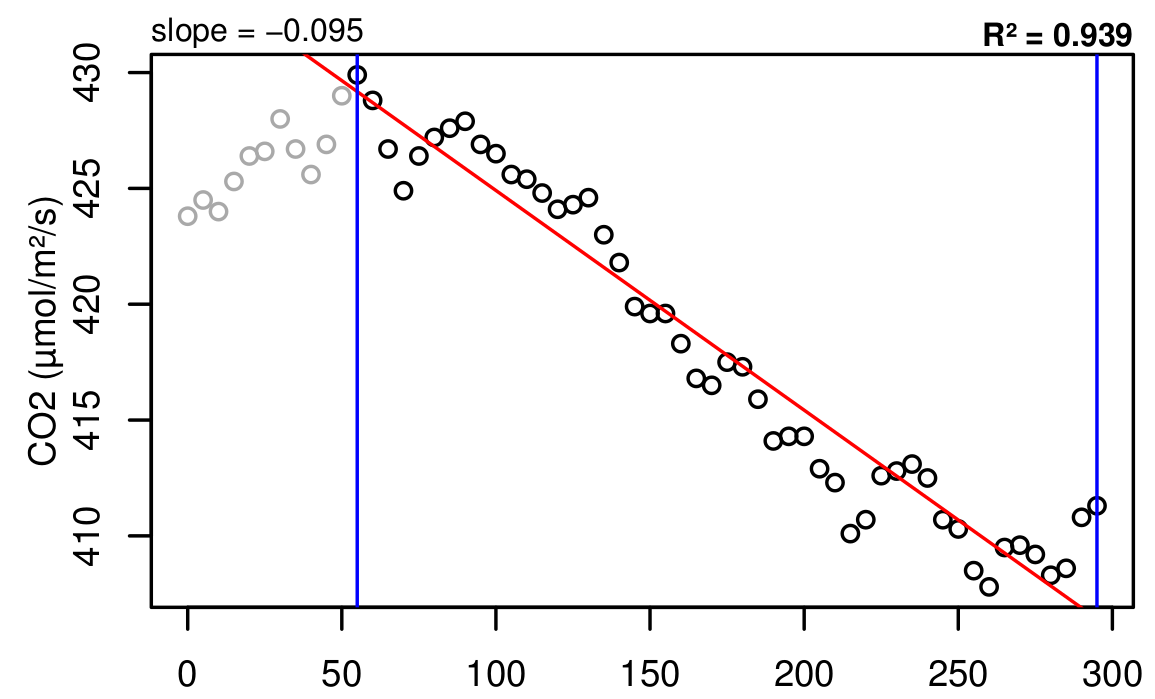
\includegraphics[width=\textwidth]{chap2/chb_ENE_reg}
		\caption{Mesure de l'échange net de l'écosystème}
	\end{subfigure}%
	\begin{subfigure}[t]{0.5\textwidth}
		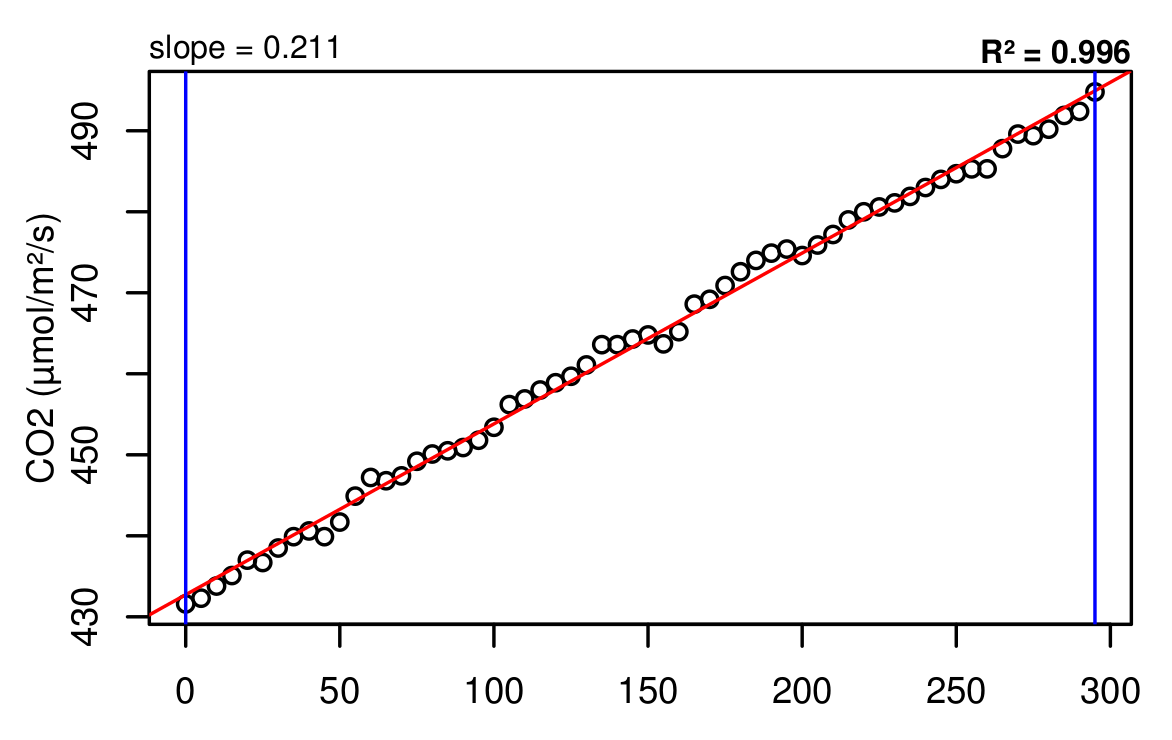
\includegraphics[width=\textwidth]{chap2/chb_ER_reg}
		\caption{Mesure de la respiration de l'écosystème}
	\end{subfigure}
%    \caption{Caption place holder}
\caption{Mesures de \coo}
\label{fig:chb}
\end{figure}


De nombreux écueils peuvent rendre une mesure inexploitable. D'abord le placement de la chambre, cela peut sembler trivial mais positionner la chambre au milieu d'herbacées et de bruyère n'est pas toujours évident. Plus anecdotiquement des sphaignes gelées, recouvrant les bords de l'embase rendent la pose de la chambre difficile voire impossible. Selon l'heure de la journée des gradients de concentrations peuvent être présent et augmenter localement les concentrations de \coo de façon importante allant jusqu'à saturer la sonde.

Au vu du volume de données acquises et souhaitant garder l'intérêt de mesure manuelle, à savoir le contrôle humain des flux et des conditions de mesure, il a été nécessaire de développer un outil de traitement facilitant le contrôle et le calcul des flux.
Ceci afin d'éviter de recourir à des seuils arbitraires (typiquement une valeur de R$^{2}$) pour le contrôle qualité des données, mais également de permettre une reproductibilité et un traçage des modifications effectuées sur les données brutes.
(donner des exemples)

\subsection{Les mesures de \chh}

\begin{figure}
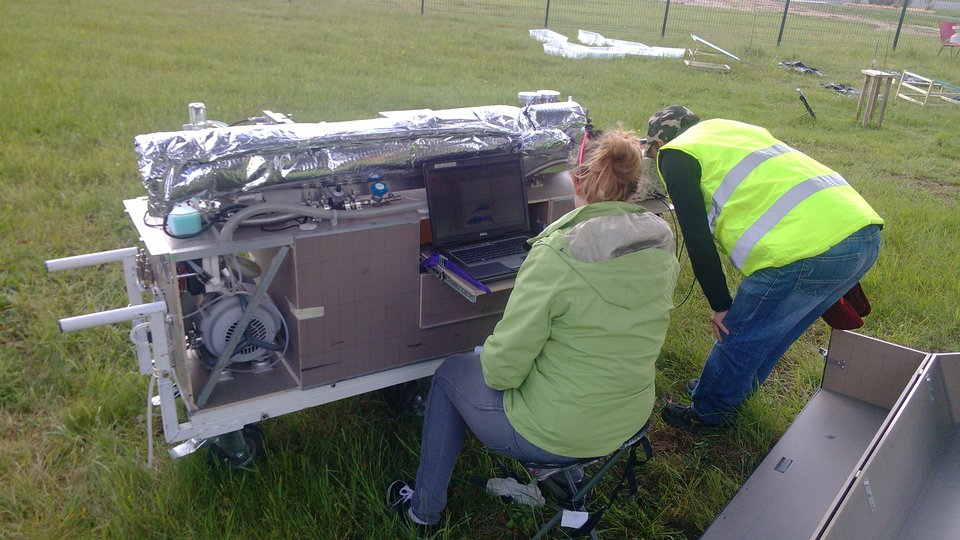
\includegraphics[width=\textwidth]{chap2/SPIRIT_terrain}
\caption{SPIRIT}
\label{fig:SPIRIT}
\end{figure}

Les mesures de \chh ont été réalisée avec une chambre aux caractéristiques similaires à celles utilisées pour les mesures de \coo à l'exception de l'interface avec l'analyseur.
La méthode de la chambre dynamique fermée a été utilisée pour réaliser ces mesures, elle diffère donc légèrement de celle utilisée pour le \coo puisqu'elle nécessite la mise en oeuvre d'un système de pompe pour transporter le gaz jusqu'à l'analyseur.
Les mesures de concentration en \chh ont été réalisée à l'aide d'un instrument développé par le LPC2E, le SPIRIT (Figure~\ref{fig:SPIRIT}).
C'est un SPectrometre Infra Rouge In-situ Troposphérique (son premier objectif étant d'être emporté lors de campagne avion ou ballon ? pour mesurer le \chh de la troposphère.).
Il permet la mesure du \chh à haute fréquence.
Le fonctionnement détaillé de l'appareil est décrit dans \cite{guimbaud2011}.

\begin{equation}
F = \frac{dX}{dt} \times \frac{P}{R \times T} \times \frac{V}{S}
\end{equation}

%QUESTIONS :
%
%*Taille des embases ? Effets de bord ?
%*Perturbation du milieu ? (Mesure de végétation, pose de la chambre, mesure pièzo...)
%*Impact de la strate arborée ?
%*Validité des profils de température ?
%Méthode de Chambre fermée (Biais ?)
%
%Améliorations ? (Lister les amélioration à faire ou non)


\section{Facteurs contrôlants}
Afin de déterminer l'impact de facteurs contrôlants sur ces flux, mesurer les flux ne suffit pas il faut également mesurer les variables environnementales dont on pense qu'elles seront des facteurs contrôlants important.
La description des techniques et matériels communs aux différentes expérimentations utilisées est développée ci-dessous.
Par contre leur mise en œuvre ou caractéristiques spécifiques, comme la fréquence des mesures, sera décrite individuellement au niveau des parties détaillant chacune des expérimentations.

\subsection{acquisitions automatisées}

Les paramètres météorologiques ont été mesurés, en un point, au centre de la tourbière (Figure~\ref{fig:carte_LG})(\textbf{carte ?}) à l'aide d'une station d'acquisition Campbell installée sur le site en 2008.
Les variables ont été acquises à une fréquence horaire jusqu'au 20 février 2014 puis toutes les demi-heures par la suite. 
Les paramètres enregistrés sont la pression atmosphérique, l'humidité relative de l'air, la pluviométrie, l'irradiation solaire, la vitesse et la direction du vent. (\textbf{détail du matos ?}).
Cette même station à également permis l'acquisition de la température de l'air et de la tourbe à \num{-5}, \num{-10}, \num{-20} et \SIlist{-40}{\cm}.
Installées à la même époque, quatre sondes \textbf{OTT ?} de mesure du niveau de la nappe d'eau permettent le suivi du niveau de la nappe dans la tourbière.

\subsection{Protocole d'estimation de la végétation}

Le suivi non-destructif d'une végétation n'est pas triviale et nécessite la mise en place de protocoles particuliers en fonction du type de végétation.
L'objectif est de pouvoir estimer une biomasse produite en impactant au minimum la végétation en place.
Pour l'ensemble des espèces végétales présentes dans les embases servant à la mesure des flux un recouvrement à été estimé, à l’œil.


\subsubsection{La strate arbustive}
Pour la strate arbustive des mesures de hauteur moyenne ont été effectuées, en mesurant depuis le niveau du sol, ou le toit des sphaignes, si elles étaient présentes, jusqu'au sommet de l'individu.
\begin{figure}
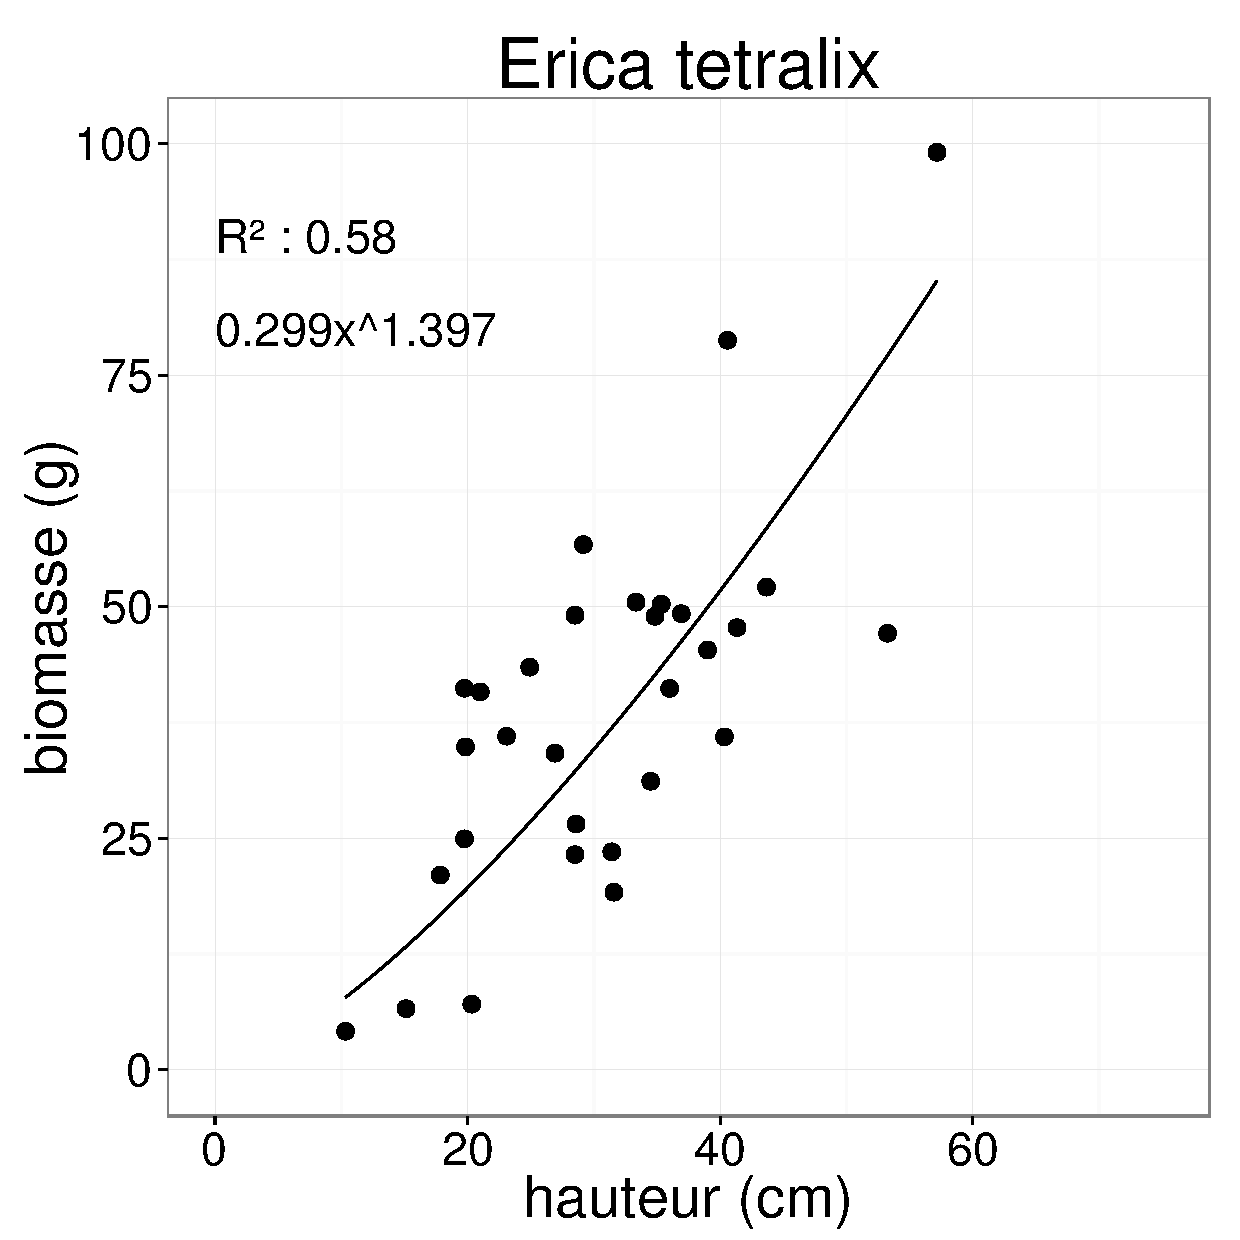
\includegraphics[width=.5\textwidth]{chap2/cal_tetra_eq}
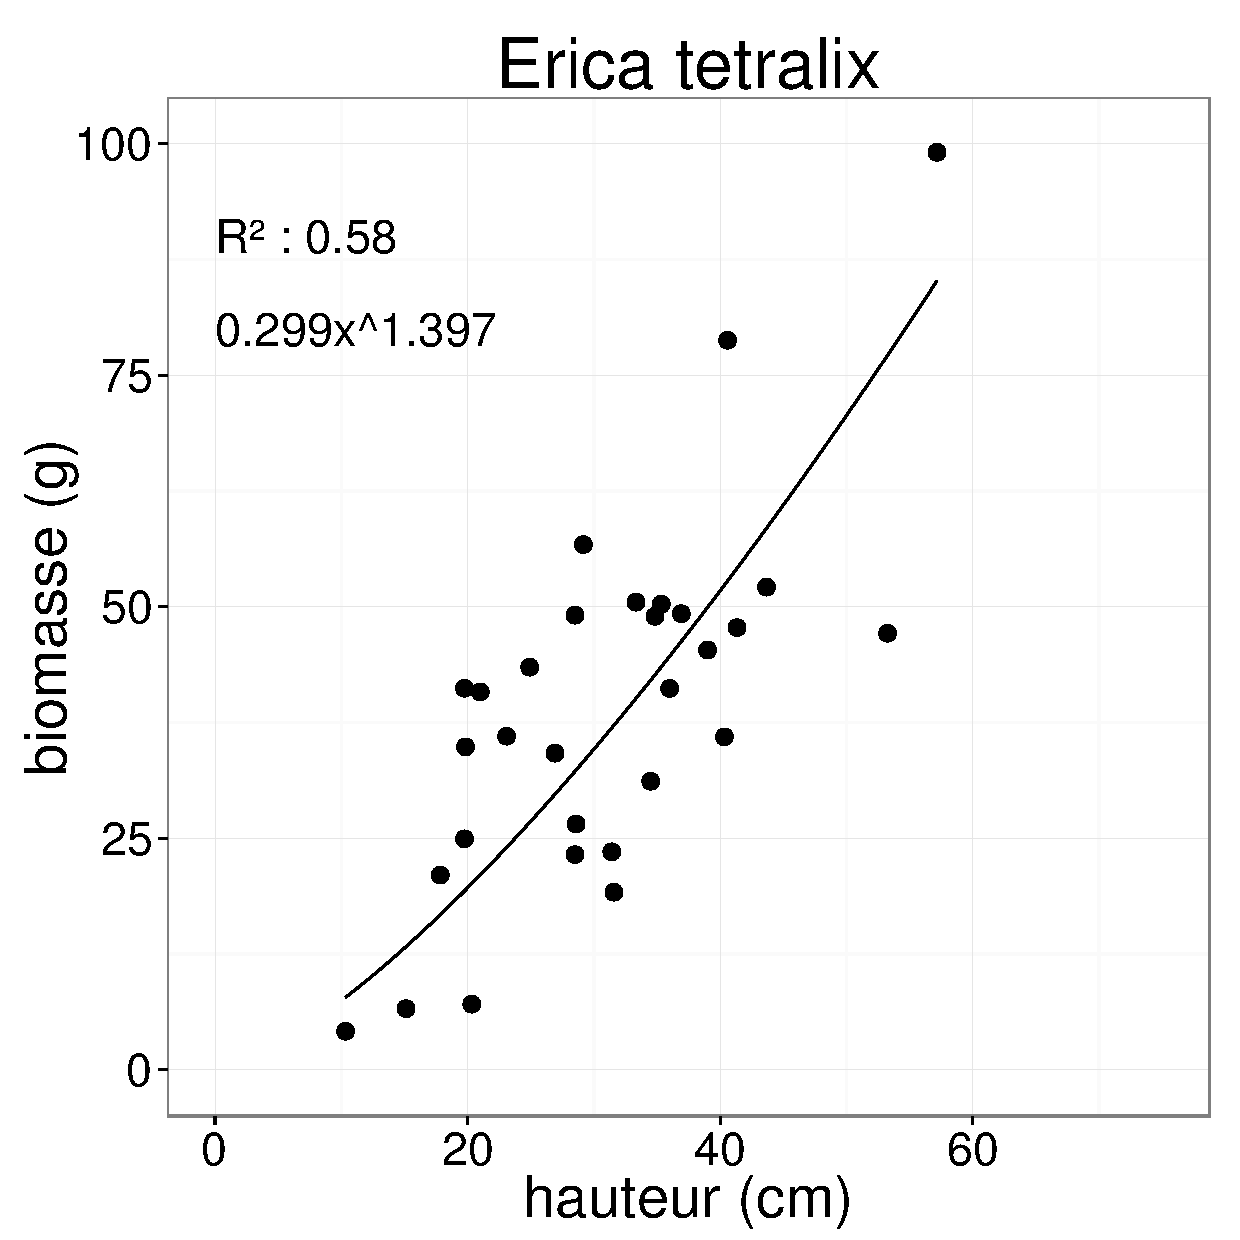
\includegraphics[width=.5\textwidth]{chap2/cal_tetra_eq}
\caption{Calibration de la biomasse en fonction de la hauteur}
\label{fig:cal_arbu}
\end{figure}

\subsubsection{La strate herbacée}
Pour la strate herbacée, en 2013, 5 individus des deux espèces majoritaires (Eriophorum vaginatum ? augustifolium ?, Molinia Caerulea) ont été marqués afin de pourvoir les mesurer plusieurs fois au cours de la saison.
Cependant les difficultés à retrouver les individus marqués couplés à la mort d'un nombre important d'entre eux n'ont pas permis d'acquérir de résultats significatifs.
En conséquence en 2014 ces deux espèces ont fait l'objet de comptage exhaustif et de mesure de hauteur moyenne.


\begin{figure}
	\centering
	\begin{subfigure}[t]{0.5\textwidth}
		\centering
		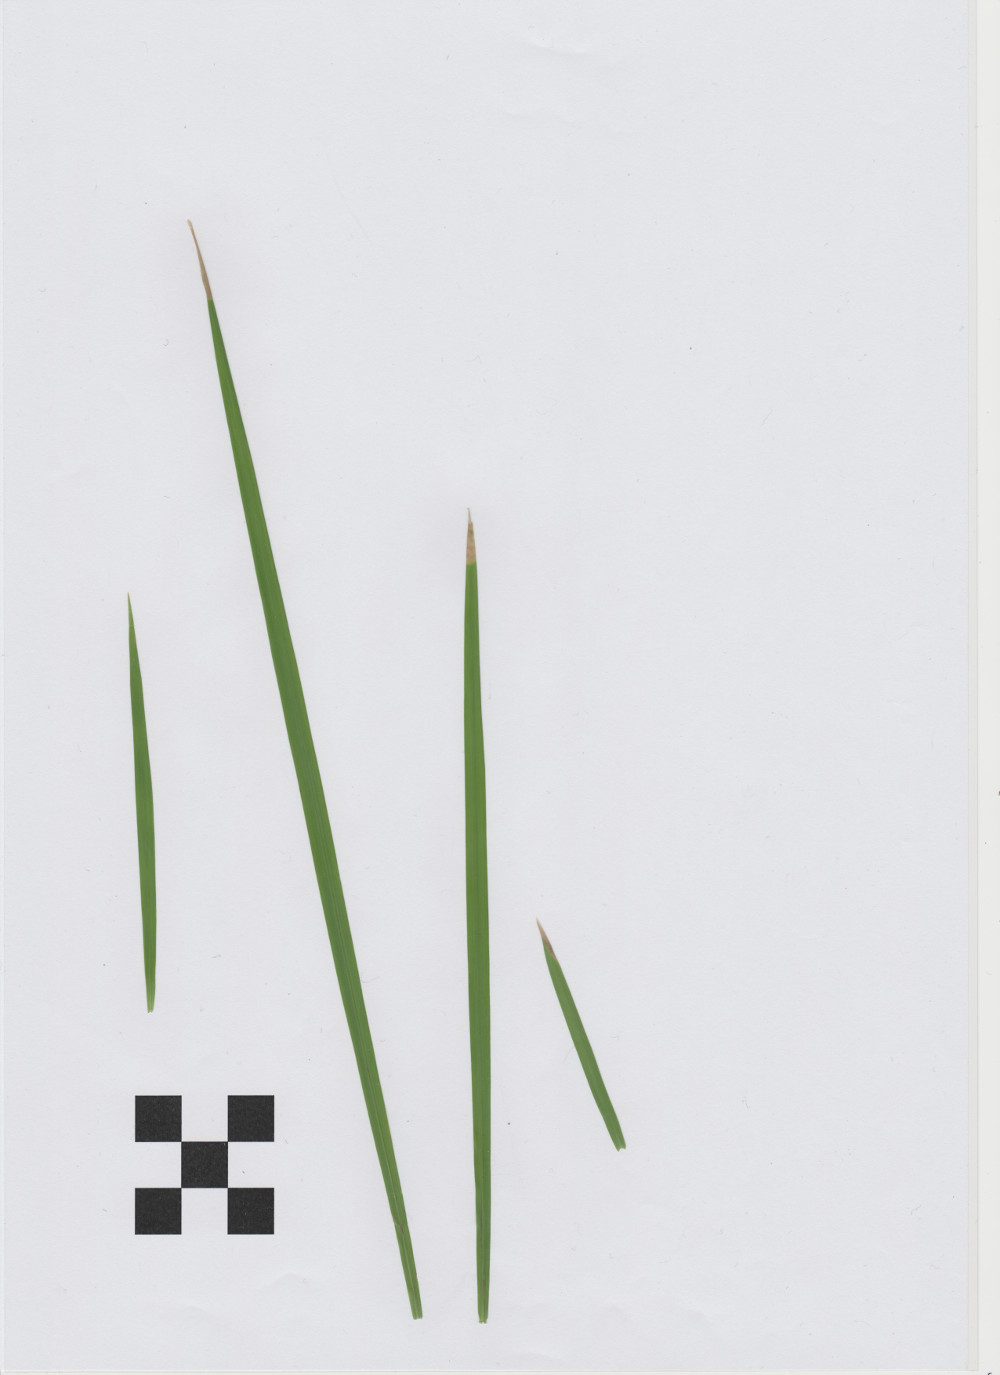
\includegraphics[width=.8\textwidth, frame]{chap2/Cch_moli_A_1to4}
		\caption{image scannée}
	\end{subfigure}%
	\begin{subfigure}[t]{0.5\textwidth}
		\centering
		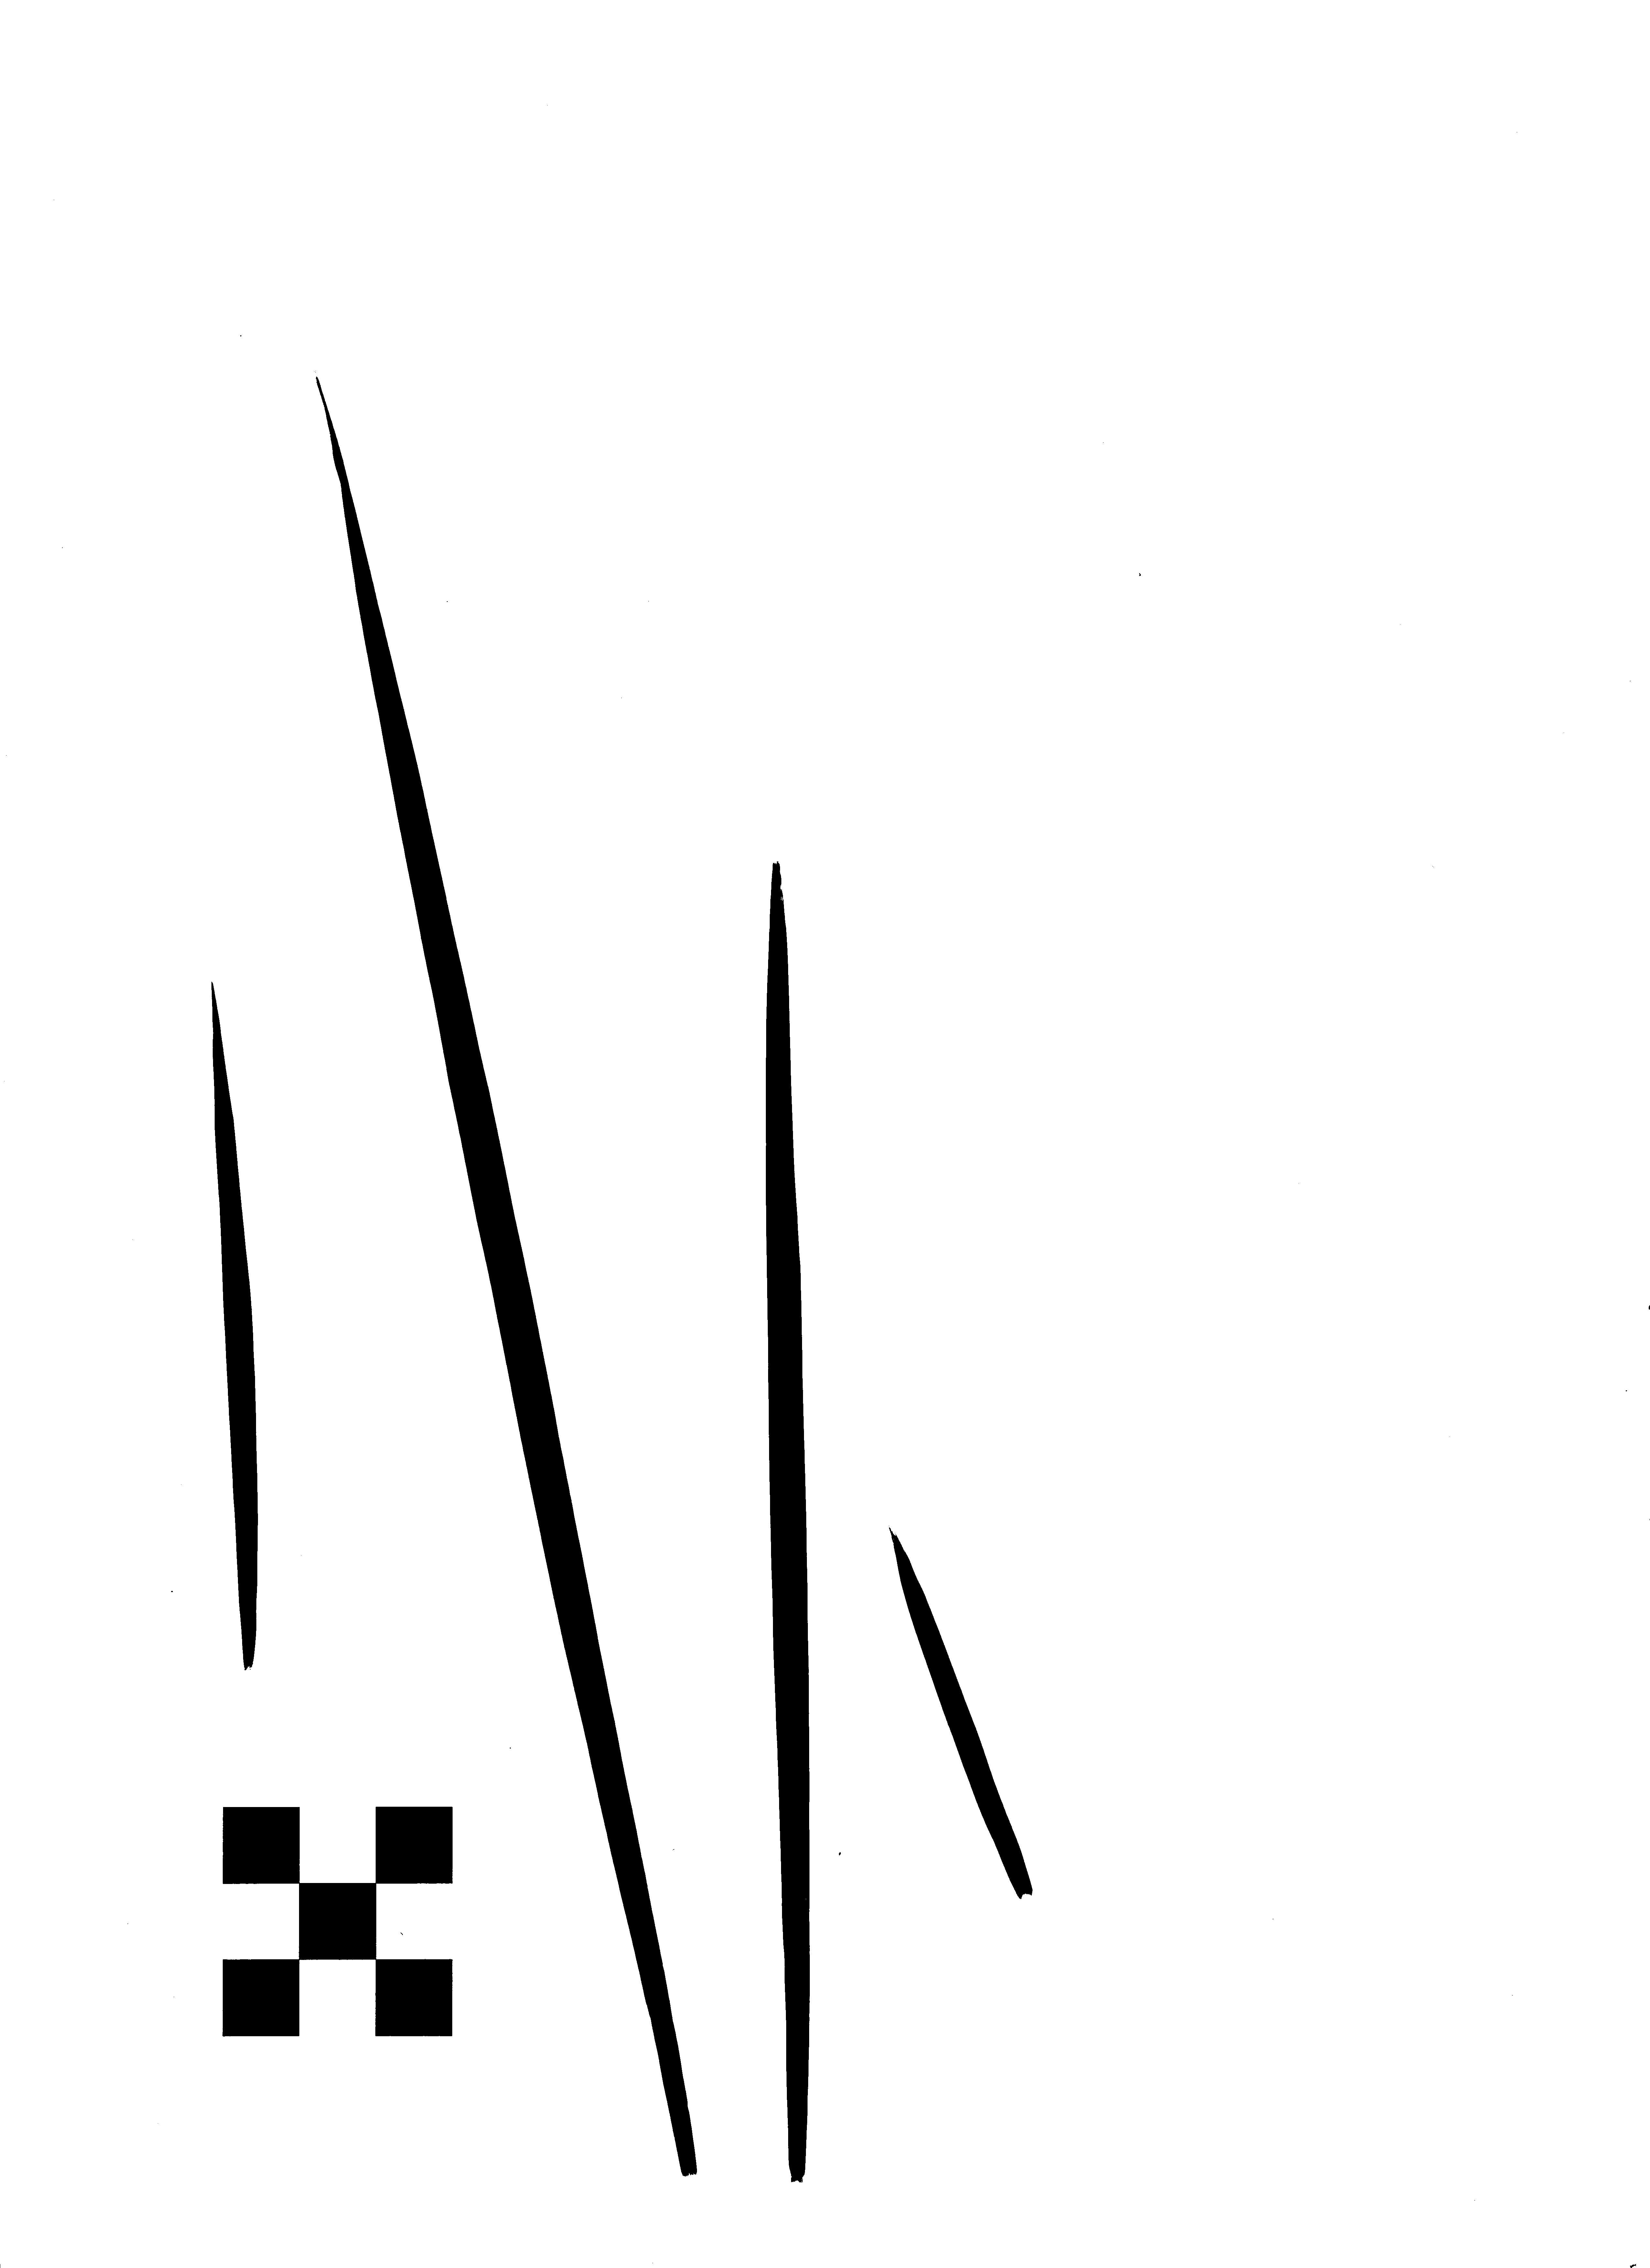
\includegraphics[width=.8\textwidth, frame]{chap2/Cch_moli_A_1to4_mod}
		\caption{image binarisée}
	\end{subfigure}
%    \caption{Caption place holder}
\caption{Scanne des feuilles}
\label{fig:scan_mol}
\end{figure}


\begin{figure}
	\centering
	\begin{subfigure}[t]{0.5\textwidth}
		\centering
		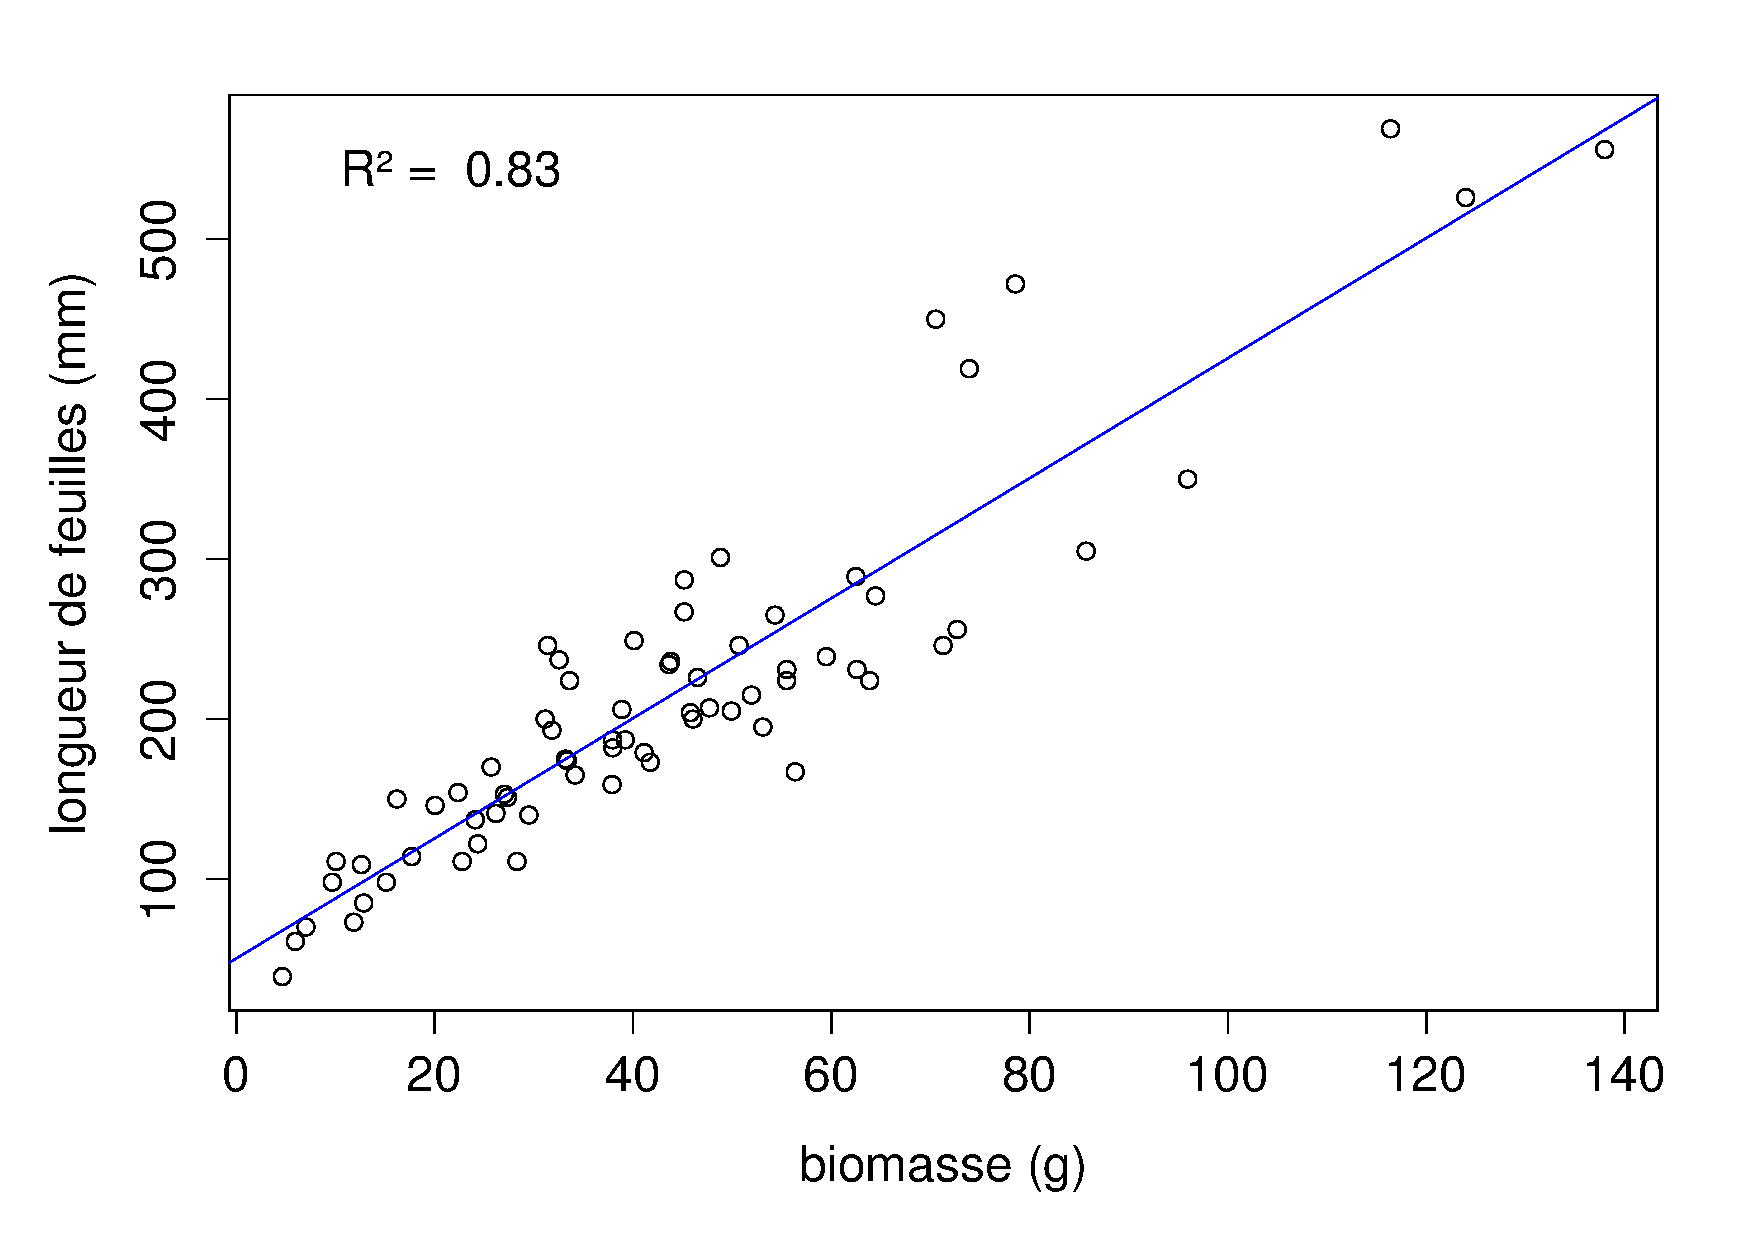
\includegraphics[width=\textwidth]{chap2/mol_lon_bioM}
		\caption{Molinia caerulea -- biomasse}
	\end{subfigure}%
	\begin{subfigure}[t]{0.5\textwidth}
		\centering
		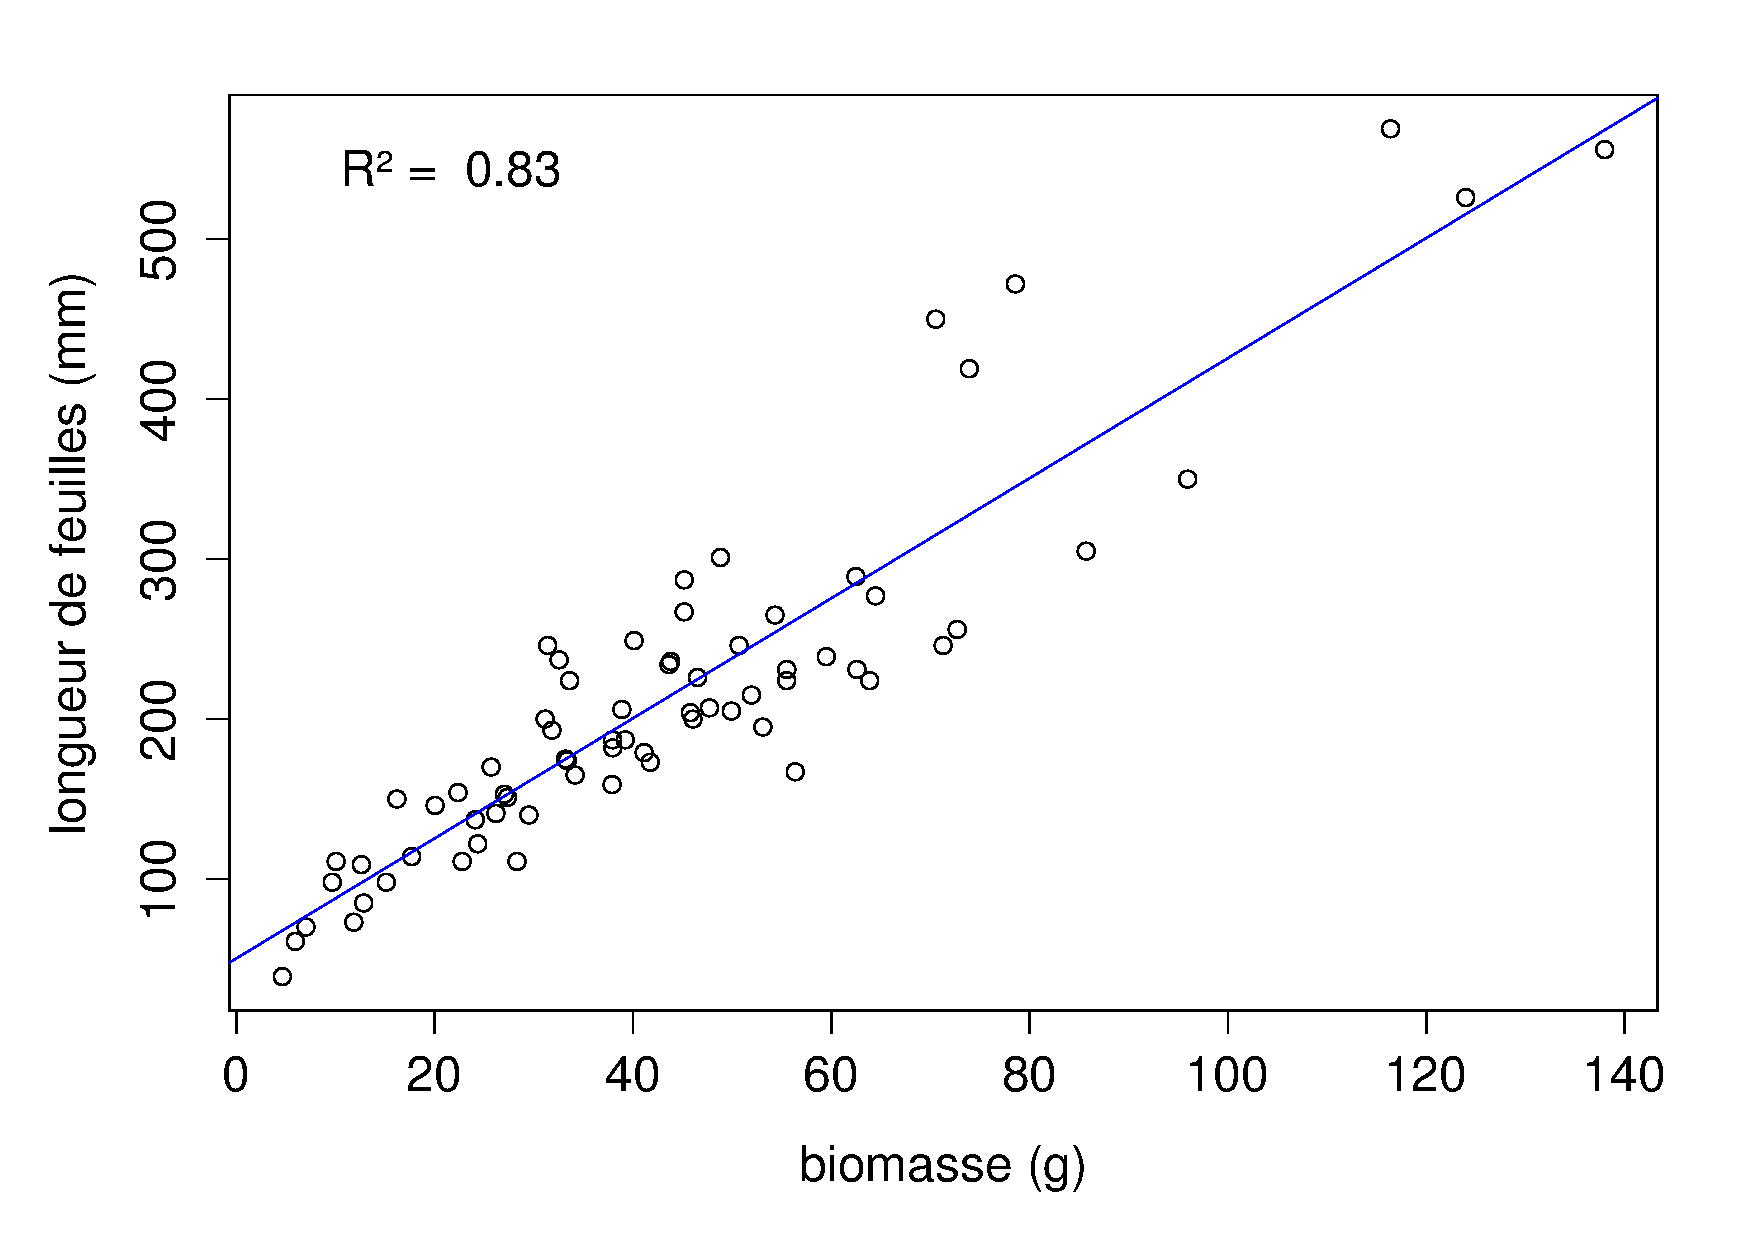
\includegraphics[width=\textwidth]{chap2/mol_lon_bioM}
		\caption{Eriophorum -- biomasse}
	\end{subfigure}
	
	
	\begin{subfigure}[t]{0.5\textwidth}
		\centering
		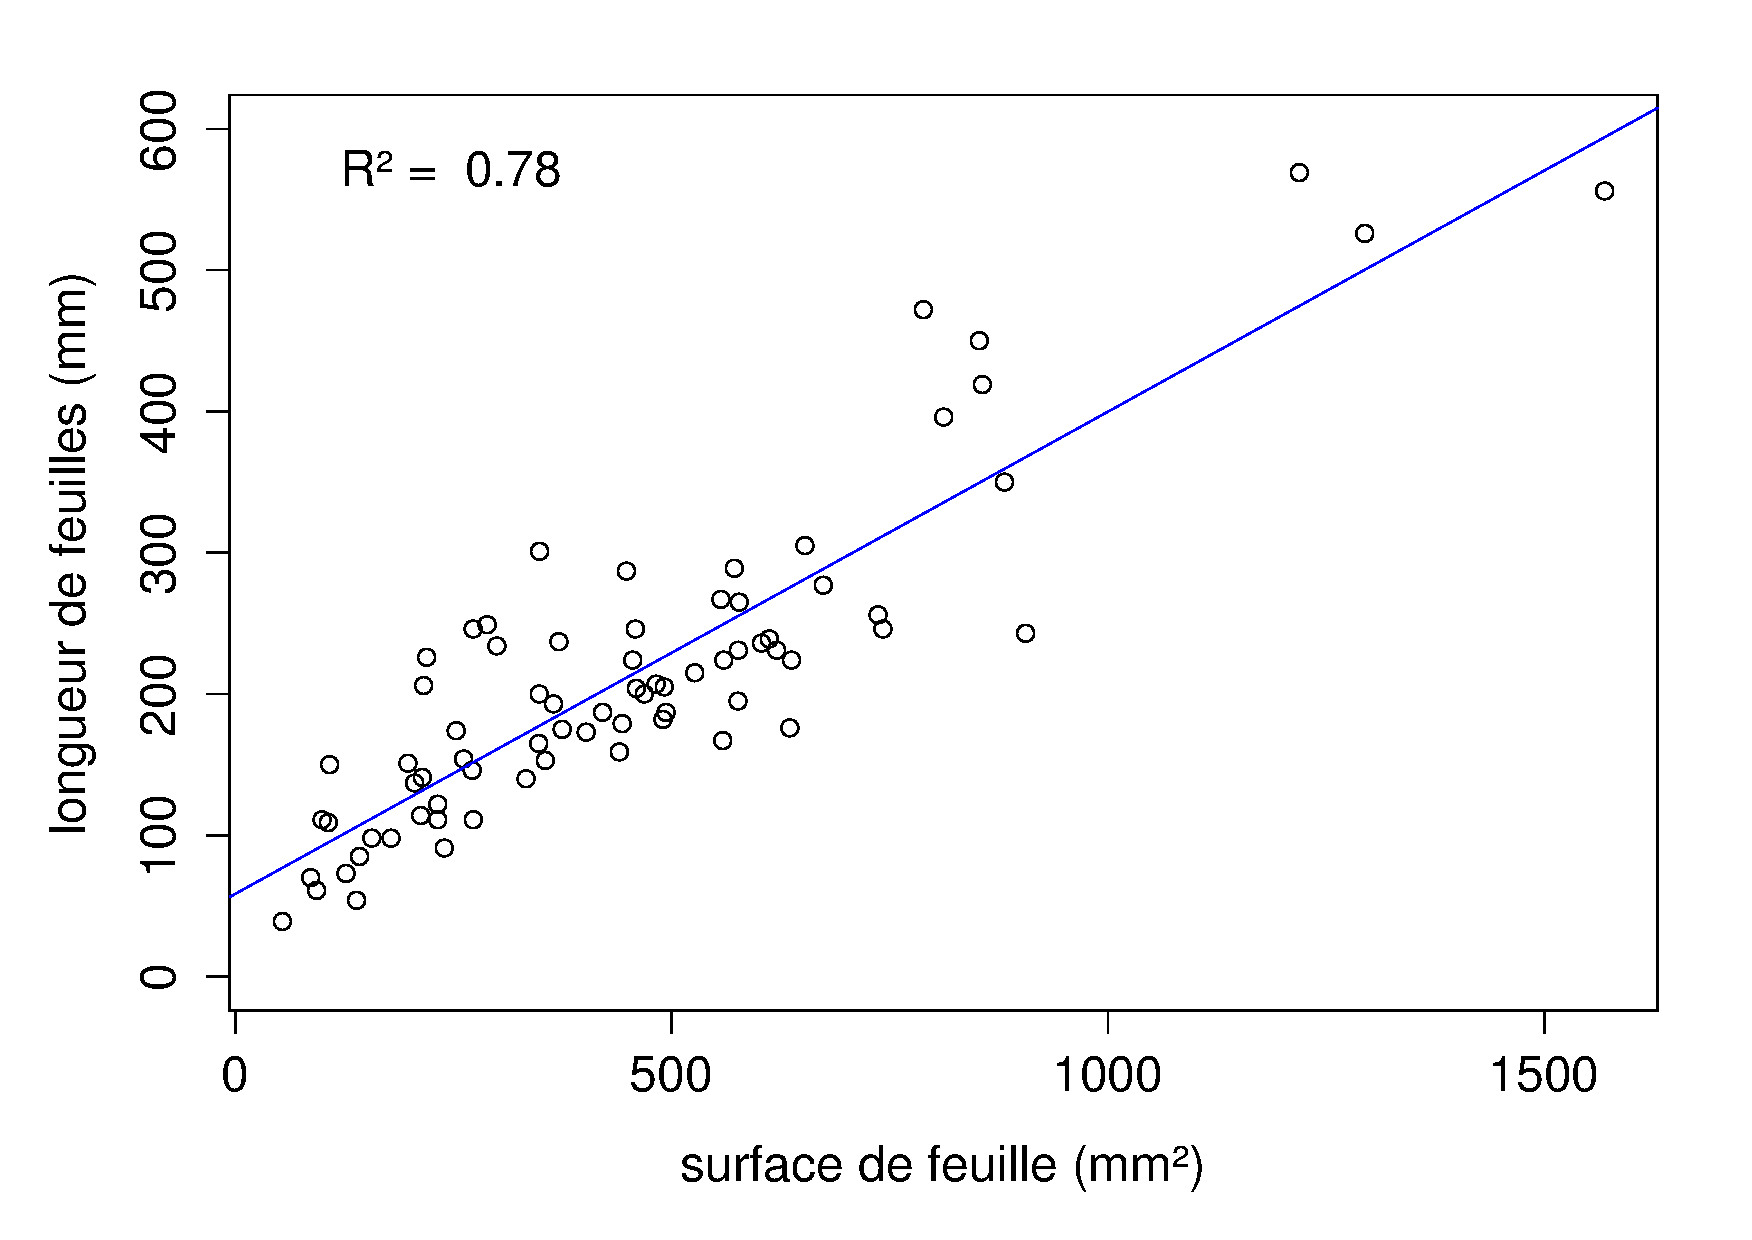
\includegraphics[width=\textwidth]{chap2/mol_lon_surf}
		\caption{Molinia caerulea -- surface}
	\end{subfigure}%
	\begin{subfigure}[t]{0.5\textwidth}
		\centering
		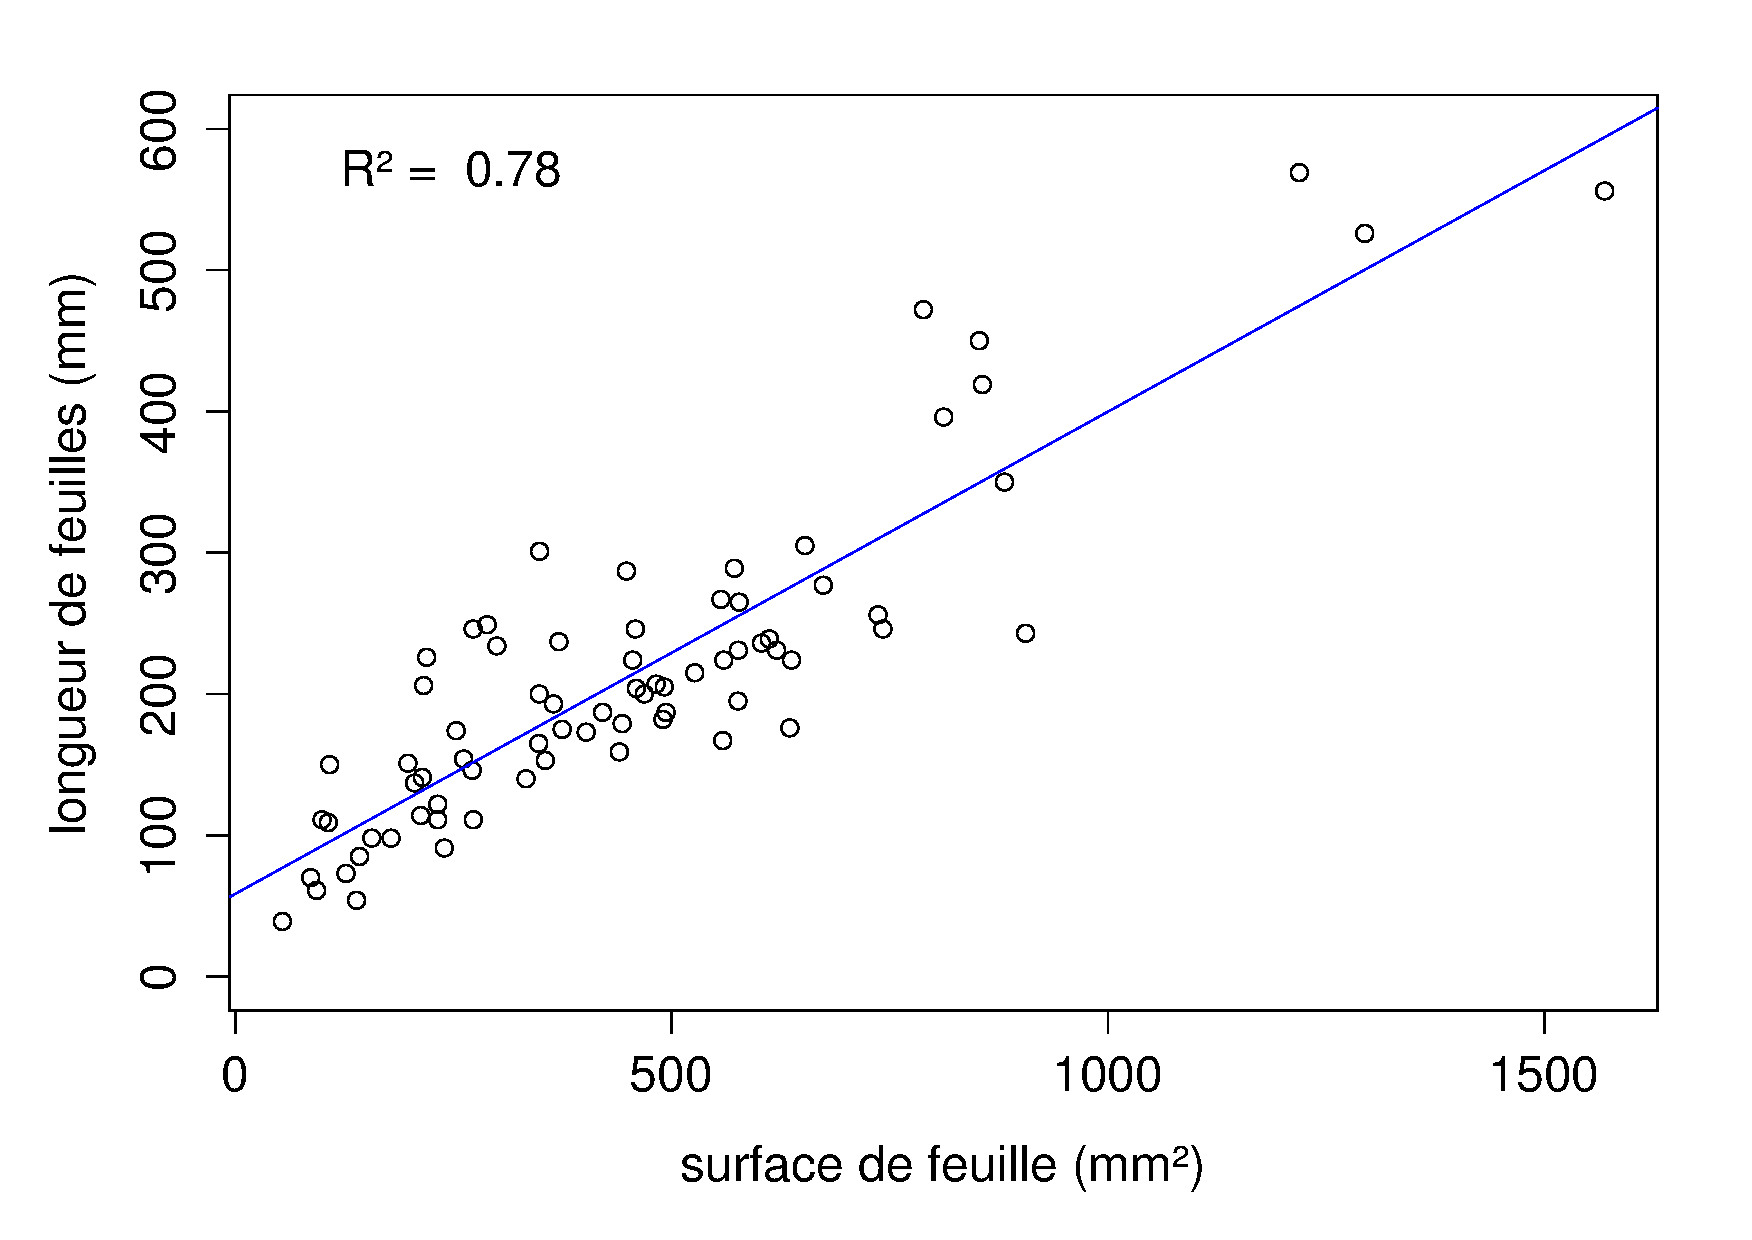
\includegraphics[width=\textwidth]{chap2/mol_lon_surf}
		\caption{Eriphorum -- surface}
	\end{subfigure}
%    \caption{Caption place holder}
\caption{Calibration de la biomasse herbacées pour \textit{molinia Caerulea} (a), pour \textit{eriophorum} (b) et de la surface de feuille pour \textit{molinia Caerulea} (c), pour \textit{eriophorum} (d) en fonction de la hauteur}
\label{fig:cal_herb}
\end{figure}


%\begin{figure}
%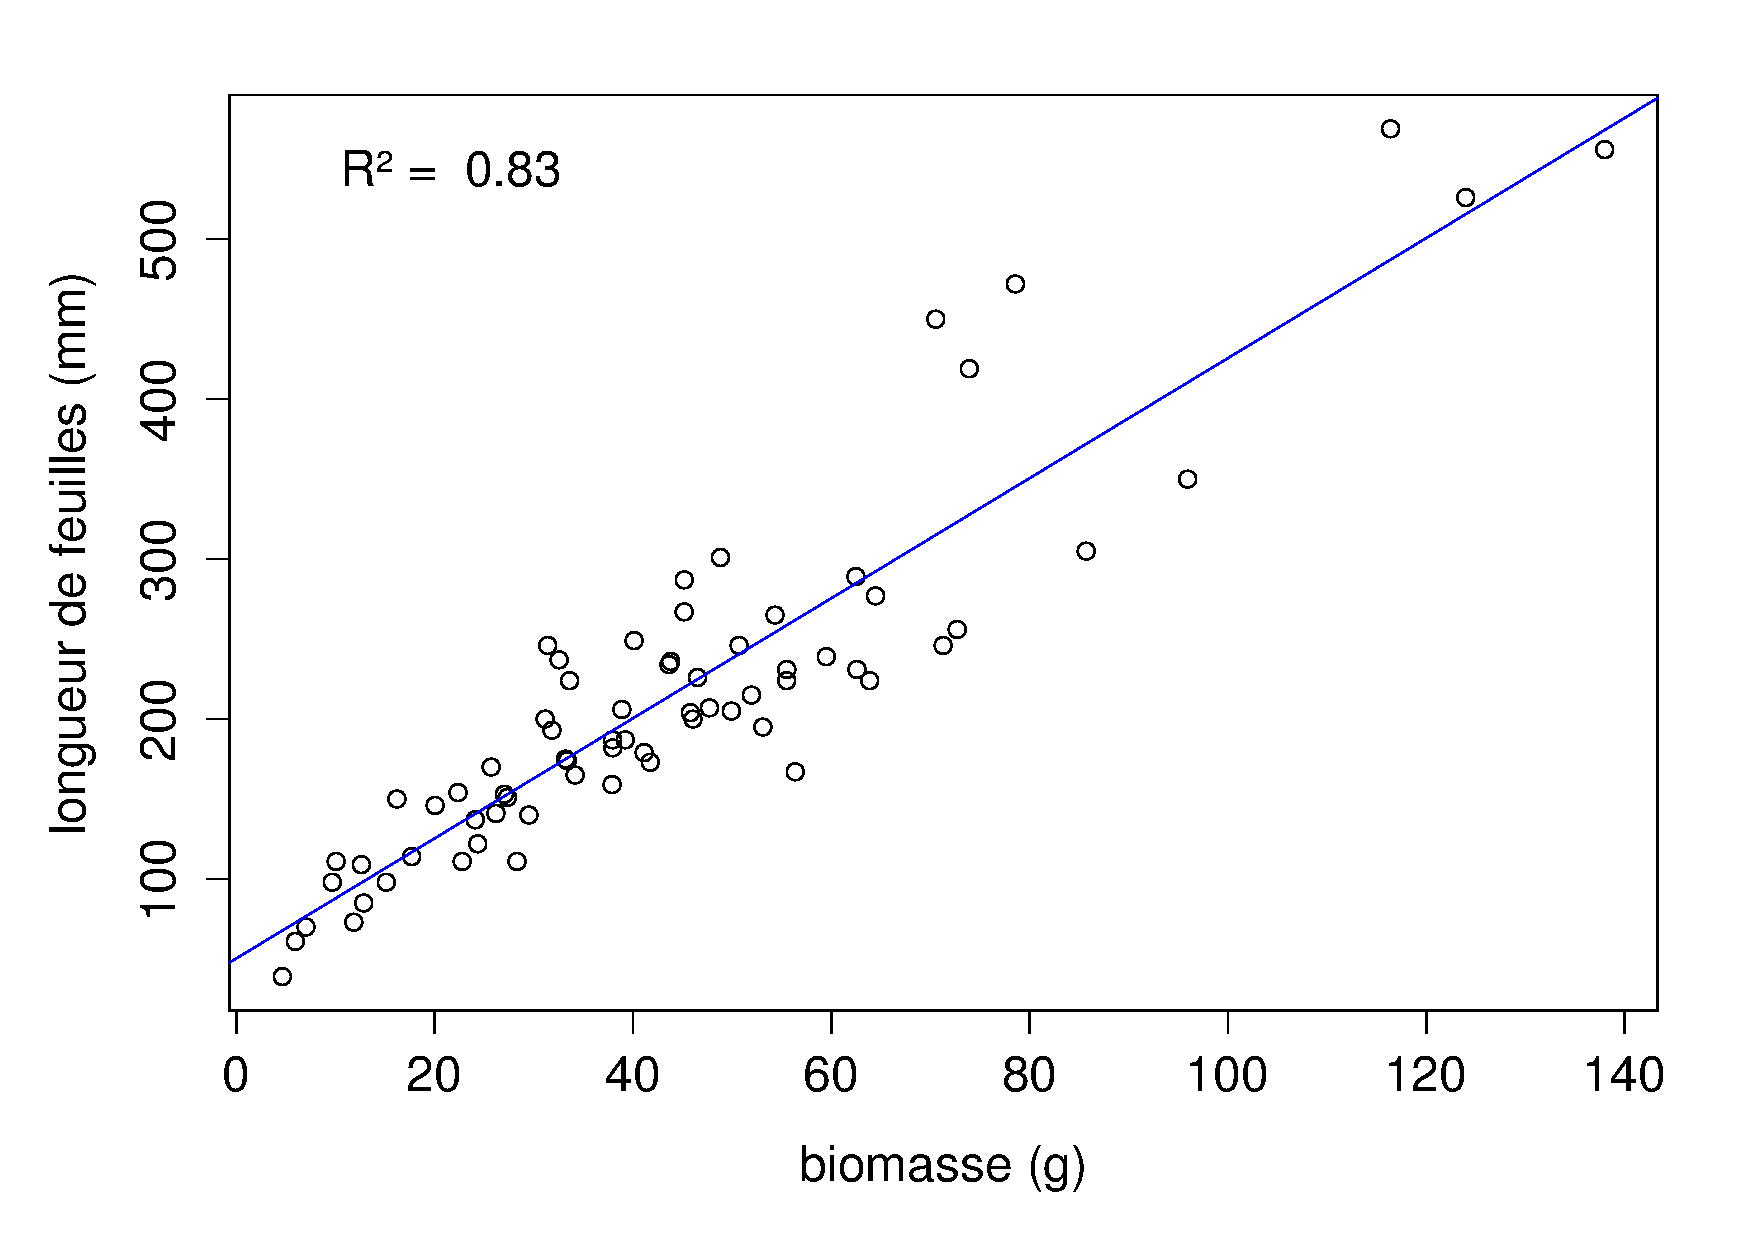
\includegraphics[width=.5\textwidth]{chap2/mol_lon_bioM}
%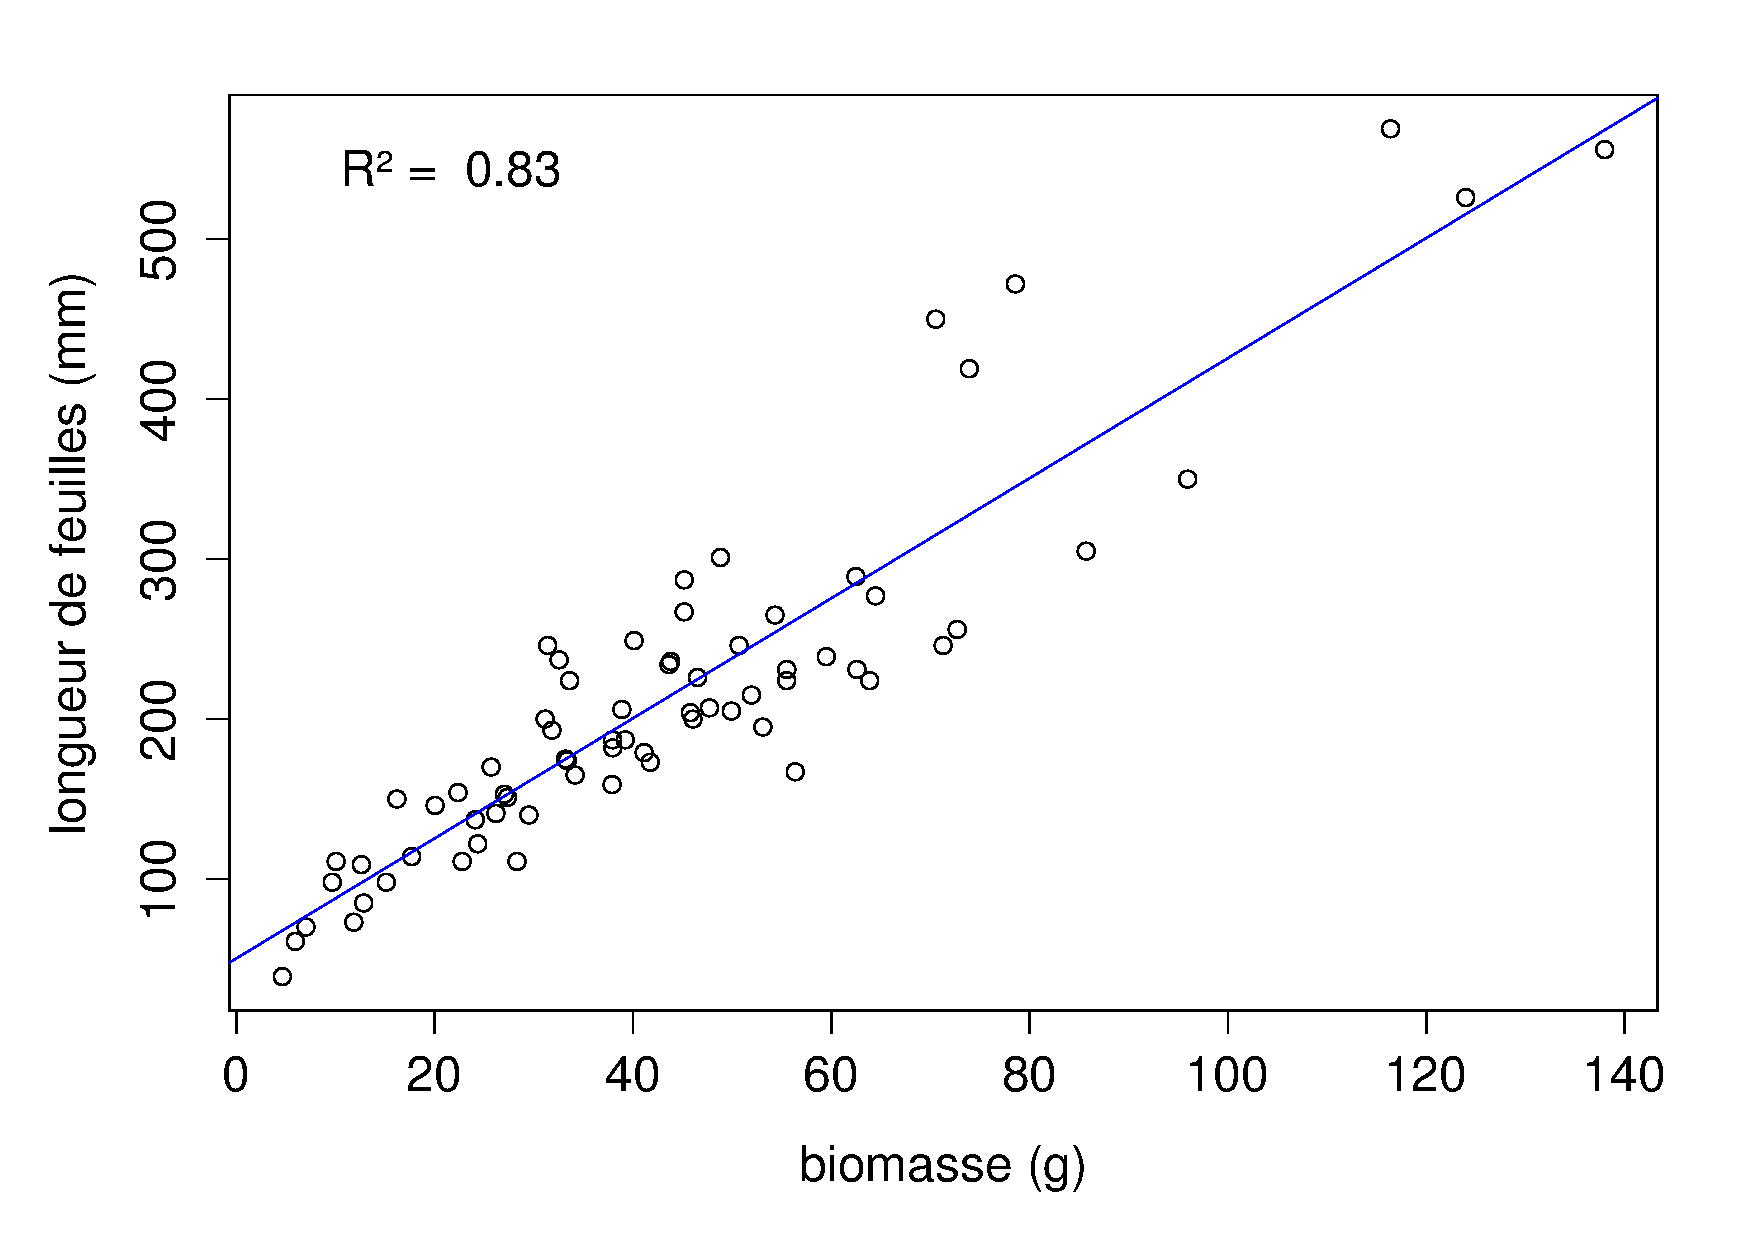
\includegraphics[width=.5\textwidth]{chap2/mol_lon_bioM}
%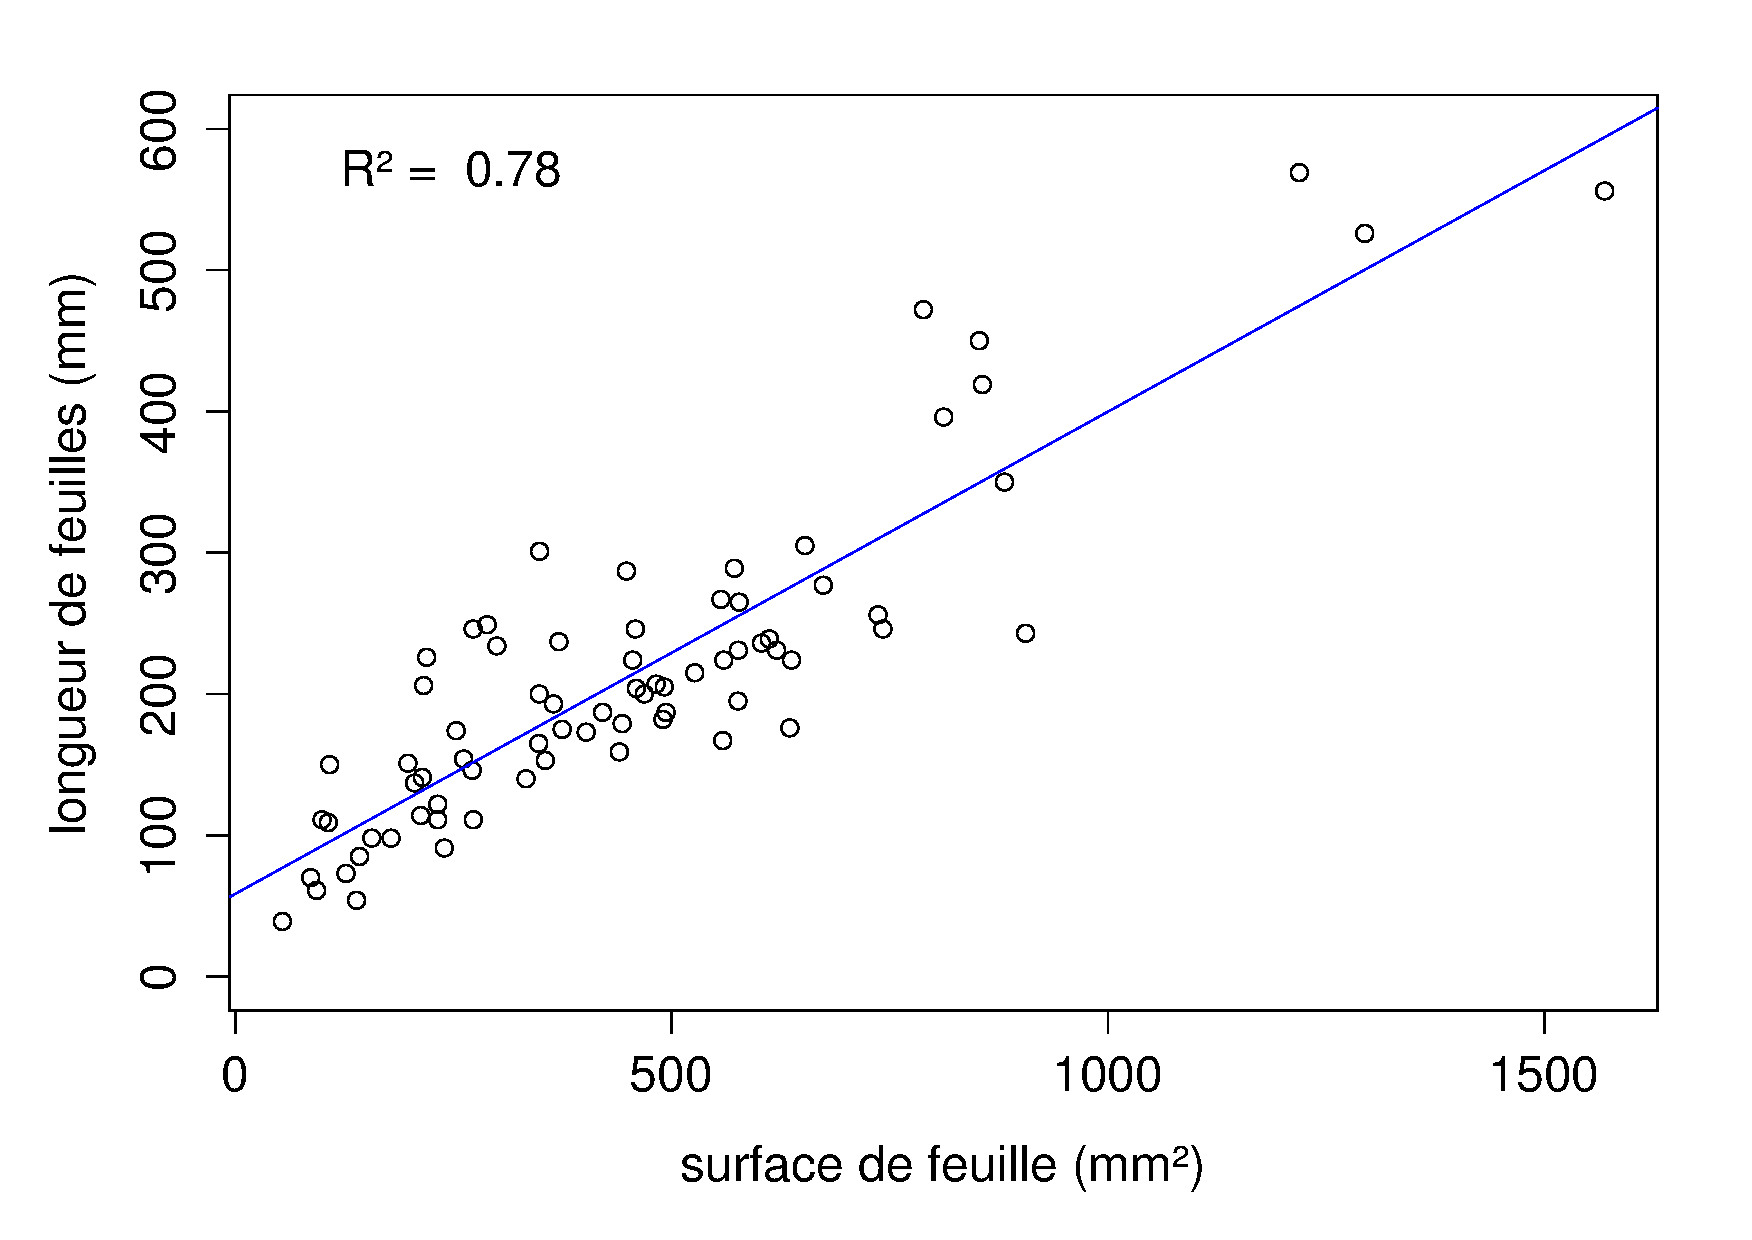
\includegraphics[width=.5\textwidth]{chap2/mol_lon_surf}
%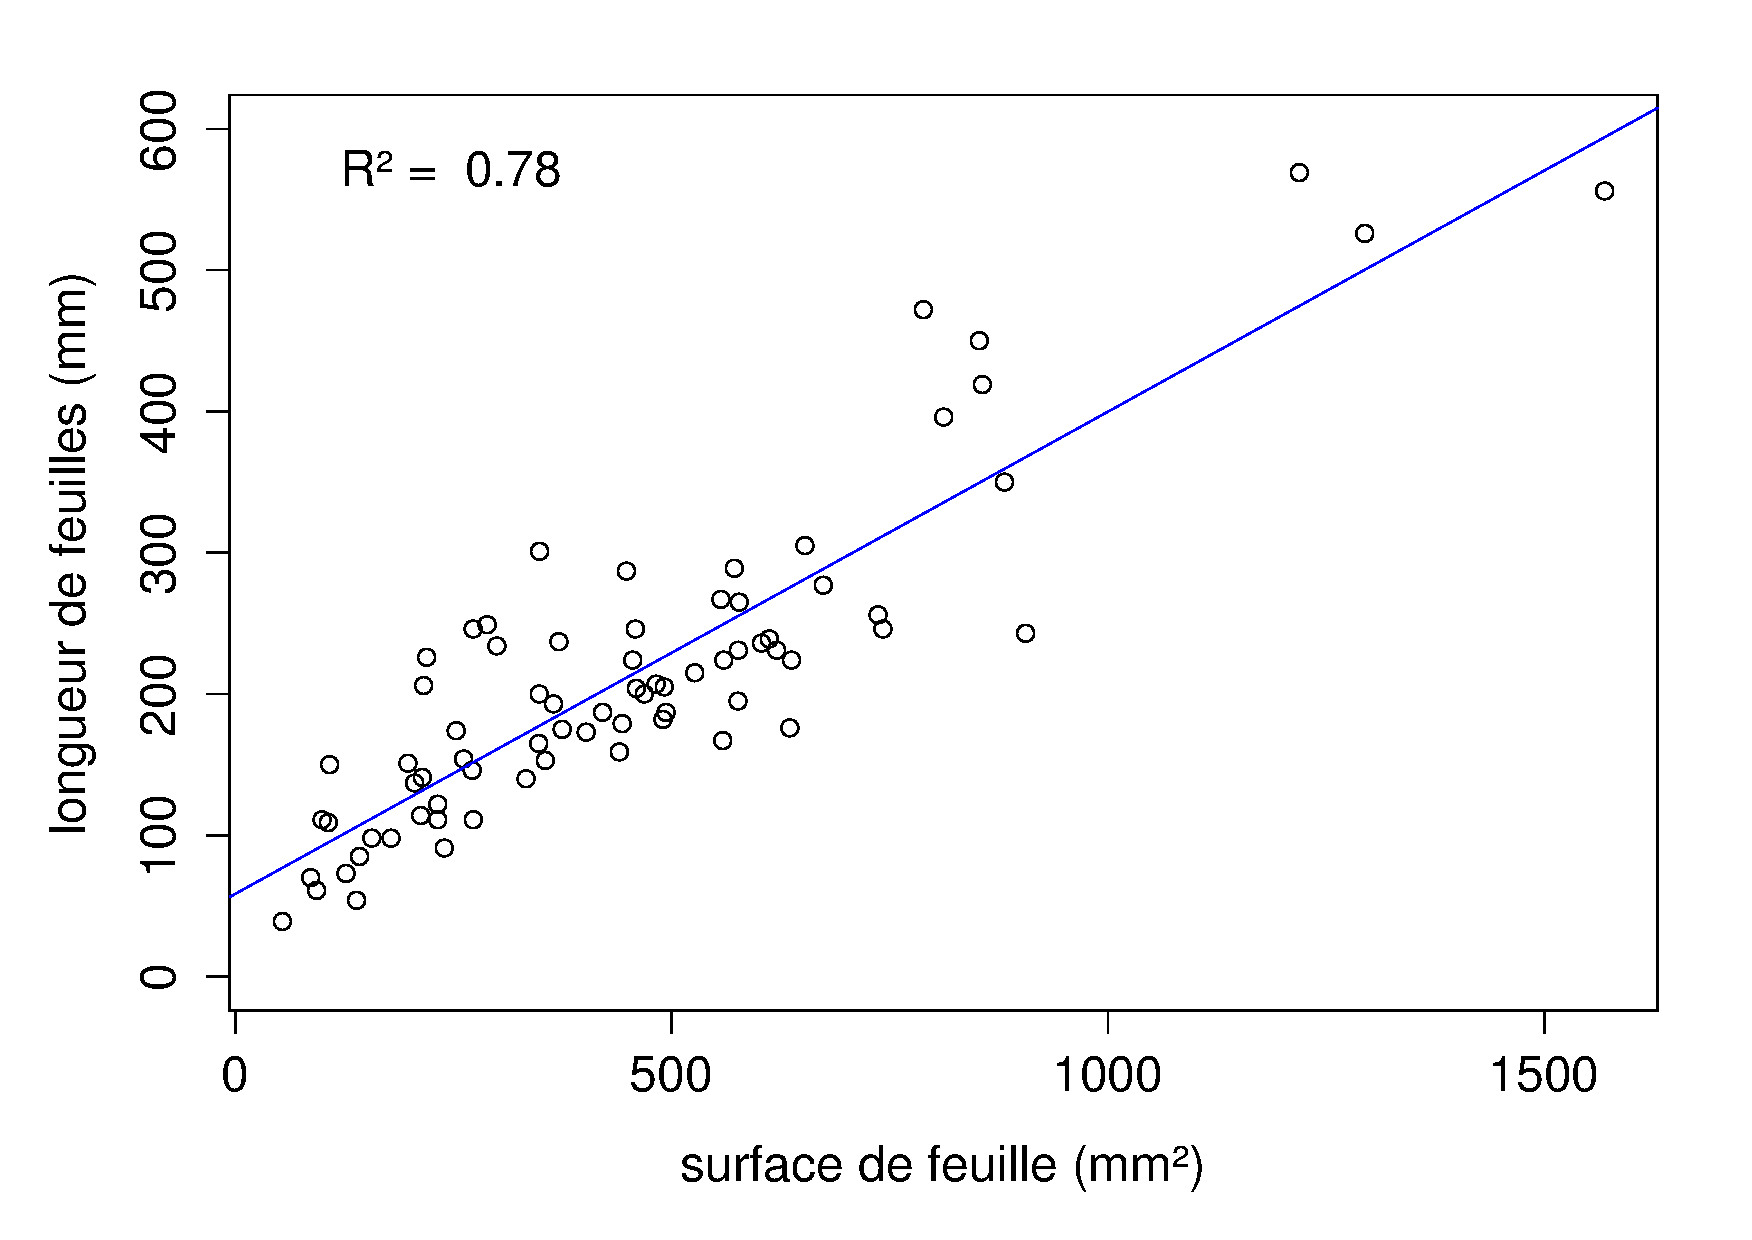
\includegraphics[width=.5\textwidth]{chap2/mol_lon_surf}
%\caption{Calibration de la biomasse herbacées pour \textit{molinia Caerulea} (a), pour \textit{eriophorum} (b) et de la surface de feuille pour \textit{molinia Caerulea} (c), pour \textit{eriophorum} (d) en fonction de la hauteur}
%\label{fig:cal_herb}
%\end{figure} %Sites d'études et méthodologies employées
% CHAPITRE 3
\chapter{Bilan de C de la tourbière de La Guette}

\minitoc

\newpage

\section{Introduction}

Parmi les écosystèmes tourbeux pour lesquels un bilan de carbone a été calculé, la majorité se situe dans les hautes latitudes \plop et/ou en montagne.
Le premier objectif de ce chapitre est d'établir le bilan de C de la tourbière de La Guette.
L'intérêt est double, d'une part car ce site est représentatif d'une grande partie des tourbières dans les perturbations qu'elle subie : son drainage et son envahissement par une végétation vasculaire (cf Chapitre 2).
D'autre part sa position en basse latitude la place dans des conditions environnementale qui, sans être identiques, peuvent se rapprocher de celles que subiront d'autres écosystèmes tourbeux suite au réchauffement climatique.
Le second objectif est de caractériser la variabilité spatiale de ces flux de GES à travers ce bilan de C.

\section{Procédure expérimentale et analytique}

\subsection{Méthodes de mesure}

\subsubsection{Mesures de flux de gaz}
\textbf{placer carte tourbière embase + quadrillage}
La mesure des flux de \coo et de \chh ont été effectué en utilisant la méthode décrite dans la partie~\ref{sec:clsd_chbr_method}.
En juin 2011, 20 placettes ont été installées\footnote{je remercie ici Sébastien Gogo pour avoir installé ces placettes sur le terrain avant même mon arrivée.} selon un échantillonnage aléatoire stratifié:
La surface de la tourbière a été divisée selon une grille de 20 mailles et un point choisi aléatoirement dans chaque maille localise chaque placette.
Cette méthode permet de conserver un échantillonnage aléatoire tout en étant assuré d'avoir une représentativité homogène du site. 
Les placettes, délimitées par des piquets, occupaient une surface de \SI{4}{\square\metre} (2$\times$\SI{2}{\metre}), à l'intérieur de laquelle ont été installé de façon permanente un piézomètre et une embase permettant la mesure des flux de gaz.
Usuellement les placettes sont séparées en groupes micro-topographique. ce qui à l'avantage de permettre une distinction des capacités sources/puits relativement fine mais qui à généralement l'inconvénient du placement proche des embases les unes des autres.
Elles peuvent également être séparées en zone dans la tourbière, haut-marais par rapport à bas-marais, ou réhabilité par rapport à non-réhabilité.
Afin de gagner en représentativité spatiale, la taille du site le permettant, il a donc été décidé de positionner des placettes sur l'ensemble du site.
De plus, du fait de l'omniprésence de végétation vasculaire, et de la taille des chambres par rapport à la micro-topographie une telle approche était difficile à mettre en oeuvre.

Les mesures de \coo ont été effectué de mars 2013 à février 2015, avec une fréquence quasiment mensuelle (20 campagnes, pour 24 mois de mesure).

Les mesures de \chh ont été effectuées avec une fréquence moindre principalement liée au difficulté de mise en oeuvre de l'instrument SPIRIT (lourd, difficilement transportable dans un milieu tourbeux).

\subsubsection{Les facteurs contrôlants}

Les mesures manuelle effectuées sont la mesure de la pression atmosphérique, du PAR, des températures du sol à différentes profondeur, de la végétation.
Des prélèvements d'eau ont également été effectué chaque mois, une mesure du pH et de la conductivité dans cette eau a été réalisée sur le terrain après les mesures de flux puis les échantillons ont été congelés avant d'être analysé en terme de concentration de carbone dissous.
Ces mesures nécessitant d'accéder aux placettes régulièrement, des planches de bois ont été utilisées comme pontons mobiles, la dispersion des placettes sur le site rendant impossible une installation plus permanente.

Les mesures automatiquement acquise via une station météo campbell sont la température de l'air, température de la tourbe à X, X et X profondeur, vitesse et direction du vent, humidité relative de l'air, irradiation solaire, pression atmosphérique.

\subsection{Modélisation du bilan de C}

\subsubsection{Démarche générale}

Afin de calculer le bilan de carbone du site il est nécessaire d'établir des modèles empiriques des flux afin de pourvoir interpoler les données acquises mensuellement sur l'ensemble des deux années de mesure.
Pour établir ces modèles empiriques les données acquises ont été moyennées par campagne de mesure.
Ceci permettant, dans un premier temps, de s'affranchir de la variabilité spatiale des flux pour se concentrer sur la variabilité temporelle.
Les relations entre flux et facteurs contrôlant ont ensuite été étudiées deux à deux.

Les flux de \coo ont été modélisé en partant de l'équation ENE = PPB - RE, et le bilan a été établi en estimant de façon séparée la PPB et la RE.
Cette séparation permettant de distinguer si une variation du bilan est liée à l'un ou l'autre des flux ou bien aux deux.
Les flux en phase gazeuse ont été modélisé en partant d'équation usuellement utilisées et dans lesquelles la température est le facteur contrôlant majeur.
Puis les résidus\footnote{Valeurs moyennes - Valeurs moyennes estimées} de ces modèles de base ont ensuite été étudiés en fonction des facteurs de contrôle restant.
Dans le cas ou une tendance est visible, le facteur est intégré.
Les modèles ont été comparés avec différents indicateurs, principalement Le R2, la NRMSE et l'AIC.
Le R$^{2}$ est utilisé comme indicateur de la proportion de la variabilité des données expliqué par le modèle, sa valeur est comprise entre 0 et 1.
La RMSE et sa normalisation par la moyenne NRMSE sont utilisés comme indicateur de l'écart entre les données mesurées et les données modélisées.
L'AIC (Akaile...) permet de déterminer si l'amélioration d'un modèle suite à l'ajout d'un paramètre est suffisamment intéressante pour que ce modèle plus complexe soit utilisé.

La température a été choisie comme base de départ à la construction des modèles de RE et PPBsat, à la fois car c'est le facteur de contrôle le plus souvent invoqué et à la fois car les corrélations avec les flux étaient les plus forte.
Concernant la respiration de l'écosystème, les températures utilisées dans la littérature sont variables.
La température qui semble le plus utilisée est la température du sol à \SI{-5}{\centi\metre}  \cite{ballantyne2014}\plop, même si d'autres, notamment la température de l'air et la température du sol à \SI{-10}{\centi\metre} le sont également régulièrement \cite{bortoluzzi2006,kim1992}.
Cette profondeur, \SI{-5}{\cm}, est régulièrement utilisée car c'est dans la tourbe, proche de la surface qu'est produit la majorité du \coo.
\textbf{production CO2 ? profils ?}
C'est également à des profondeurs relativement faibles que se situent la majorité des racines \plop qui peuvent contribuer à la respiration du sol \textbf{(de l'écosystème?)} pour 35 à \SI{60}{\percent} \cite{silvola1996,crow2005}.

Après cette phase de calibration, les facteurs de contrôle utilisés dans les modèles ont été interpolés au pas de mesure de la station météo présente sur le site, c'est à dire à l'heure.
L'interpolation étant soit une simple interpolation linéaire entre les données mensuelles, soit une relation avec les facteurs acquis par la station météorologique.
À l'aide de ces interpolations et des équations les flux ont ensuite été recalculés sur les 2 années de mesure.

Enfin ces modèles ont été évalués sur des données issues d'une autre expérimentation.On ne parle pas ici de validation car les données utilisées bien qu'indépendante du jeu de données utilisé pour la calibration n'ont pas été acquise suivant un protocole identique, notamment au niveau de la répartition des embases sur le site.


\subsubsection{La Production Primaire Brute}

\begin{figure}
\centering
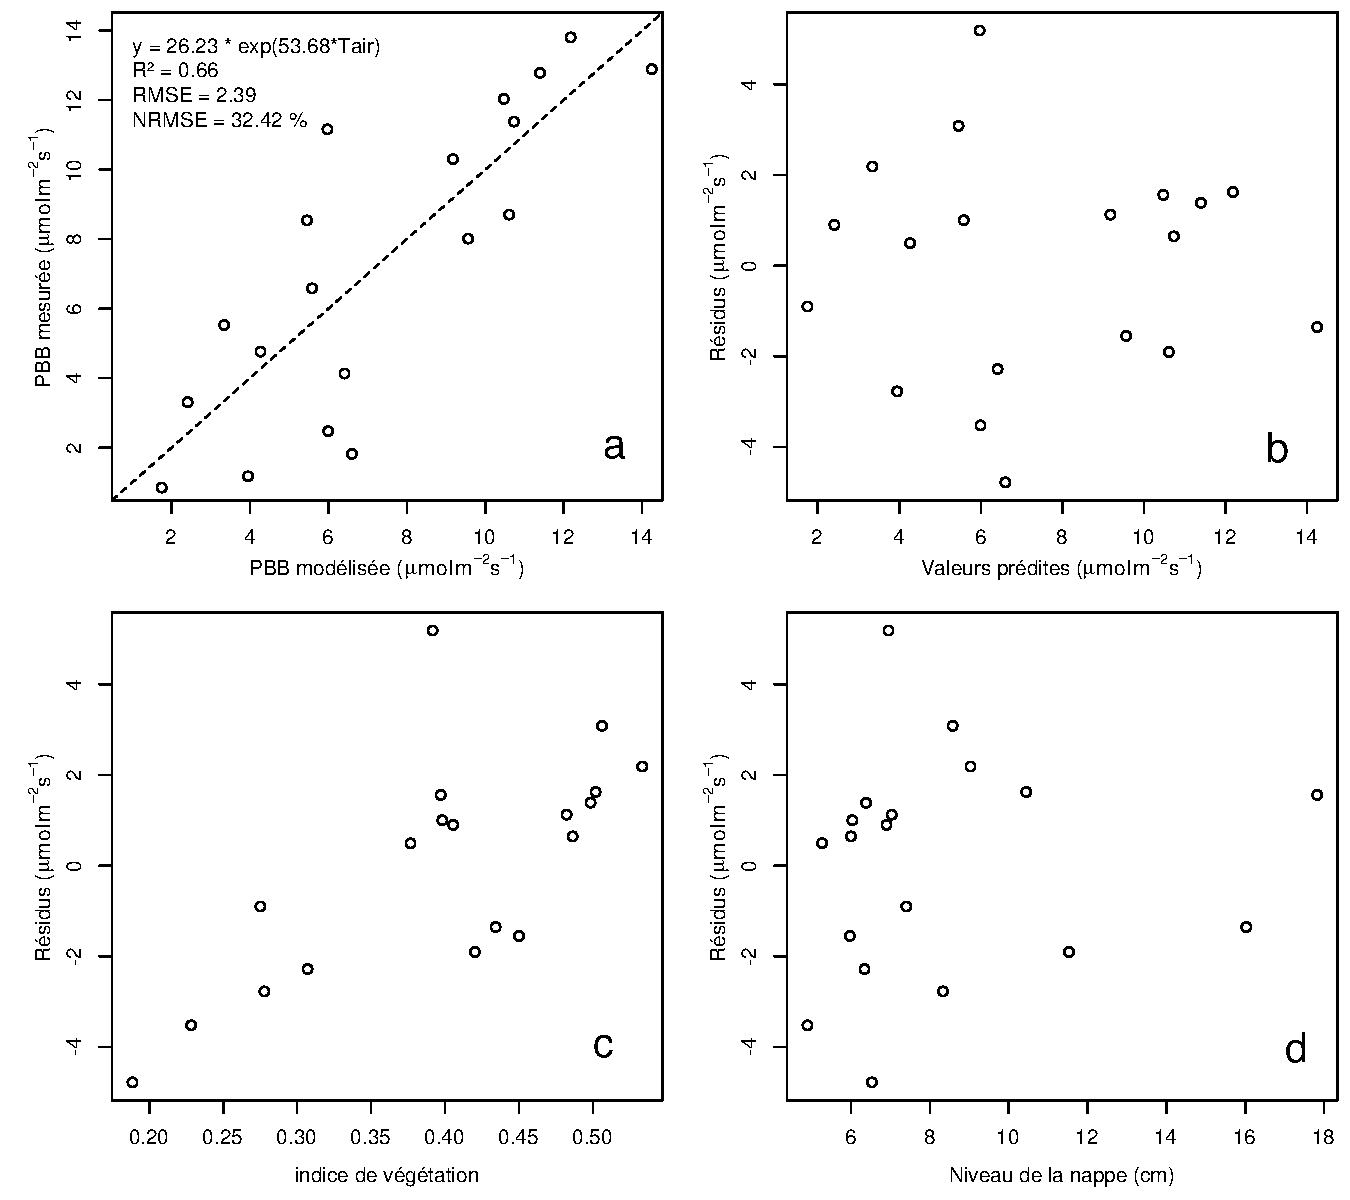
\includegraphics[width=\textwidth]{chap3/GPPsat_Tair_mesmod}
\caption{PPBsat modèles Tair utilisant l'équation~\ref{eq:juneTair}}
\label{fig:PPBsat_Tair_mdl}
\end{figure}

L'estimation de la PPB se fait en deux étapes.
Dans un premier temps on estime le potentiel maximum de photosynthèse à un instant donné dans des conditions de lumière saturante (PPBsat).
Ce potentiel peut varier avec les conditions environnementales et a été déterminé en utilisant l'équation de \cite{june2004} qui relie la vitesse de transport des électrons photosynthétique à lumière saturante à la température :

\begin{equation}\label{eq:juneTair}
PPBsat = a * exp(\frac{Tair - b}{c})^2
\end{equation}

Avec a la vitesse de transport des électrons photosynthétique à lumière saturante, b la température optimale pour ce transport et c la différence de température à laquelle à laquelle PBBsat vaut e$^{-1}$ de sa valeur à la température optimale.

L'utilisation de l'équation de June seule, avec la température de l'air comme variable explicative de la PPBsat, permet d'expliquer 66 \% des variations observées (Figure~\ref{fig:PPB_Tair_mdl}-a).
Les résidus de ce modèle se répartissent de façon relativement homogène (Figure~\ref{fig:PPB_Tair_mdl}-b).
Corrélés avec l'indice de végétation IV, ils présentent une tendance linéaire croissante (Figure~\ref{fig:PPB_Tair_mdl}-c), mais ne présentent pas de tendance particulière avec le niveau de la nappe (Figure~\ref{fig:PPB_Tair_mdl}-d)
Afin de prendre en compte cette tendance linéaire le modèle est adapté :

\begin{equation}\label{eq:juneTairIV}
PPBsat = (a * IV) * exp(\frac{T - b}{c})^2
\end{equation}

\begin{figure}
\centering
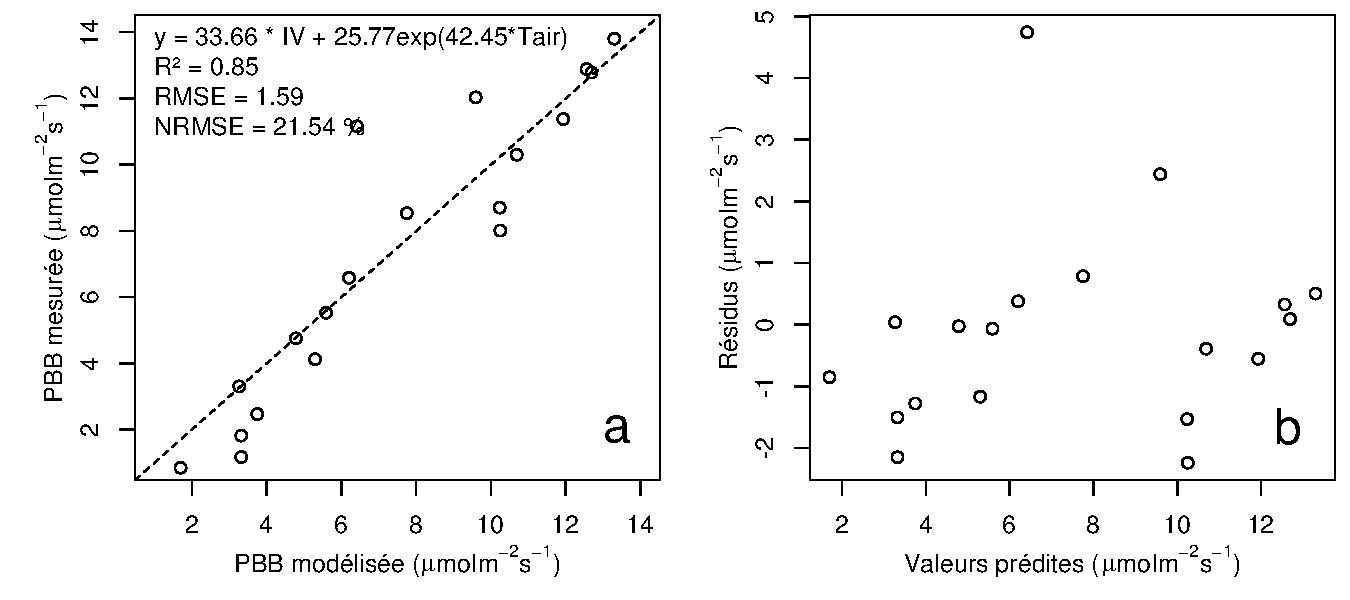
\includegraphics[width=\textwidth]{chap3/GPPsat_TairIV_mesmod}
\caption{PPBsat modèles Tair utilisant l'équation~\ref{eq:juneTairIV}}
\label{fig:PPBsat_TaIV_mdl}
\end{figure}

Cette nouvelle équation permet d'expliquer une part plus importante des variations de PPBsat (R$^{2}$ = 0,85) et augmente la proximité entre les données mesurées et les données modélisées (La RMSE diminue) (Figure~\ref{fig:PPBsat_TaIV_mdl}).
Les résidus de cette équation semblent répartis de façon moins homogène que précédemment, avec d'avantage de résidus présent entre \num{-1} et \num{-2} qu'entre \num{1} et 2, ainsi qu'un point de valeur supérieur à \num{4}.
Le biais reste malgré tout léger au regard de l'amélioration apportée.

À partir de ce potentiel à lumière saturante, la PPB est estimée en prenant en compte la luminosité.
On utilise l'équation~\ref{eq:PPB_bubier} proposée par \cite{bubier1998} et régulièrement et souvent utilisée \cite{bortoluzzi2006,worrall2009}:

\begin{equation} \label{eq:PPB_bubier}
PPB = \frac{PPBsat * a * PAR}{PPBsat + a * PAR}
\end{equation}

\begin{figure}
\centering
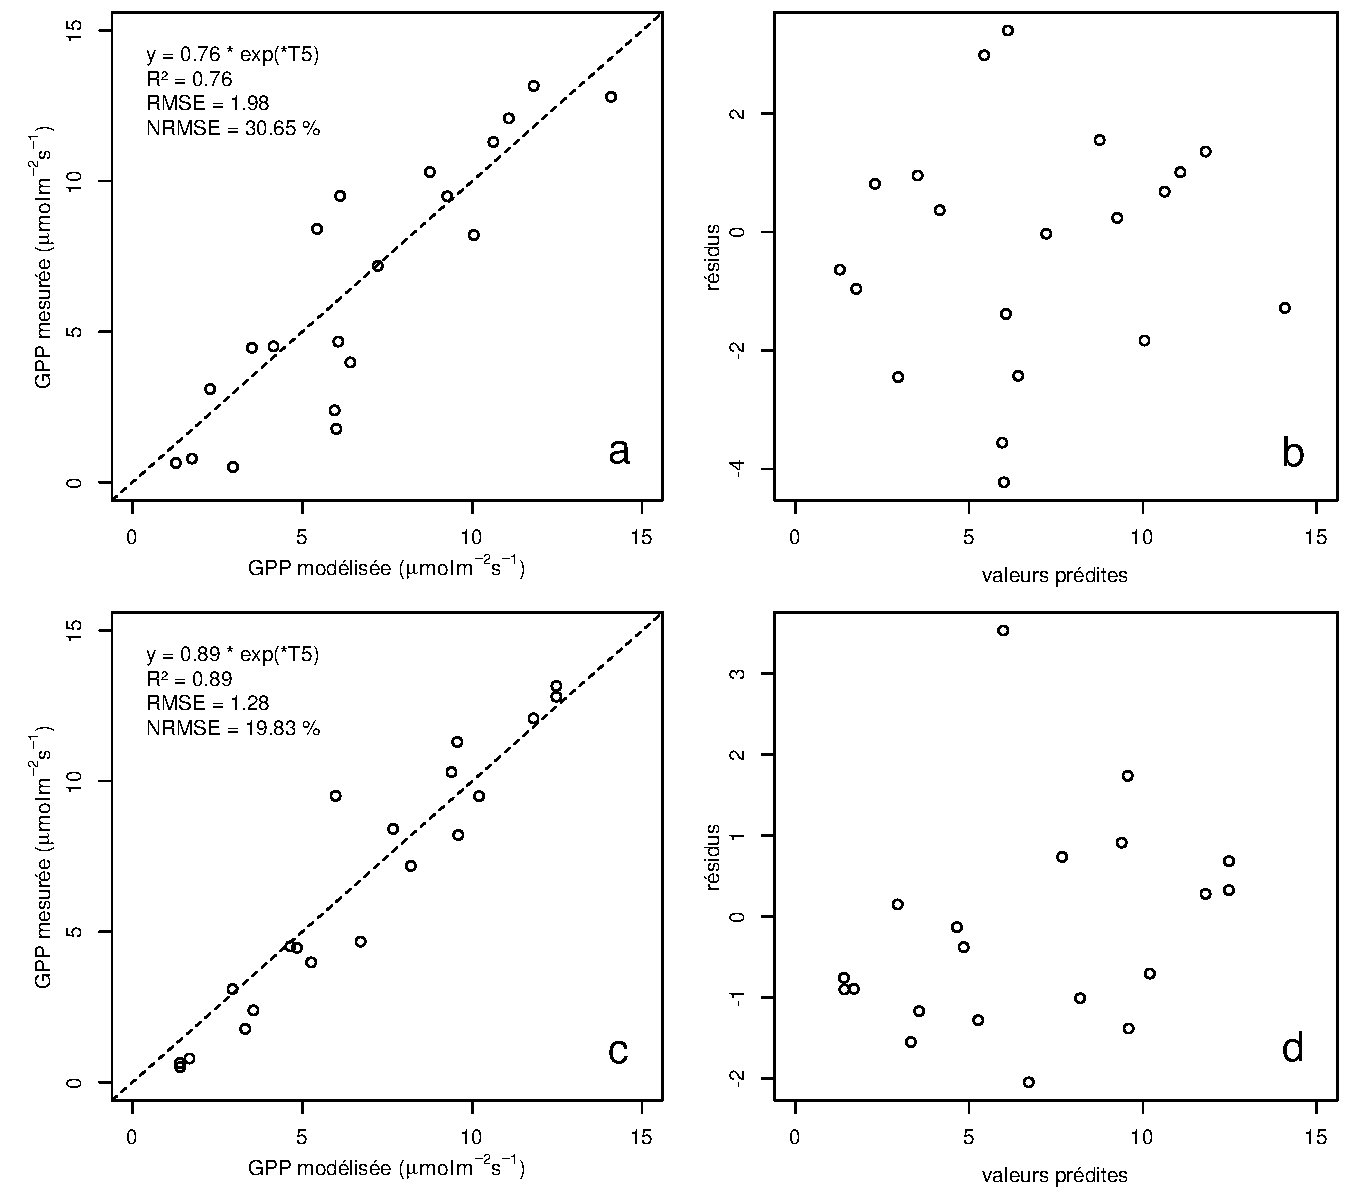
\includegraphics[width=\textwidth]{chap3/GPP_mdl_mesmod}
\caption{PPB modèles Tair}
\label{fig:PPB_Tair_mdl}
\end{figure}

La PPB calculée à partir de l'équation~\ref{eq:juneTair} présente des résidus relativement homogène avec cependant d'avantage de points situés entre \num{-2} et \num{-4} qu'entre \num{2} et \num{4} (Figure~\ref{fig:PPB_Tair_mdl}--a,b).
Une observation similaire peut être faire pour PPB calculé à partir de l'équation~\ref{eq:juneTairIV}, avec cependant des résidus resserrés entre \num{-2} et \num{2} et un point un peu plus extrême(Figure~\ref{fig:PPB_Tair_mdl}--c,d).

\subsubsection{La Respiration de l'Écosystème}

%%%%%%%%%%%%%%%%%%%%% RE

La RE est estimée directement à partir des données acquises moyennées en partant de la température connue pour contrôler une grande partie de ce flux.
Différents modèles ont été testés parmi les plus souvent utilisés (linéaire, exponentiel, arrhénius).


Les variations de la RE moyenne au cours du temps suivent les variations saisonnières de la température.

\begin{equation} \label{eq:RE_T}
RE = a*exp(b*T)
\end{equation}

La température de l'air utilisée dans un modèle exponentiel permet d'expliquer une grande partie, 90 \%, des variations de la respiration de l'écosystème (Figure~\ref{fig:ER_mdl}--a).
Les résidus de cette équation semble répartis de façon non-biaisée, pas de tendance dans le nuage de point (Figure~\ref{fig:ER_mdl}--b).
Une légère tendance, moins claire que pour la PPBsat, est visible entre les résidus et l'indice de végétation.
Très souvent utilisée, la température à \SI{-5}{\centi\metre} donne des résultats proche mais moins bons notamment avec une hétéroscédasticité des résidus.
La tendance des résidus avec l'indice de végétation est ici moins marqué encore qu'avec la température de l'air.
Dans les deux cas, le gain possible en ajoutant un paramètre semble limité et peu pertinent.

\begin{figure}
\centering
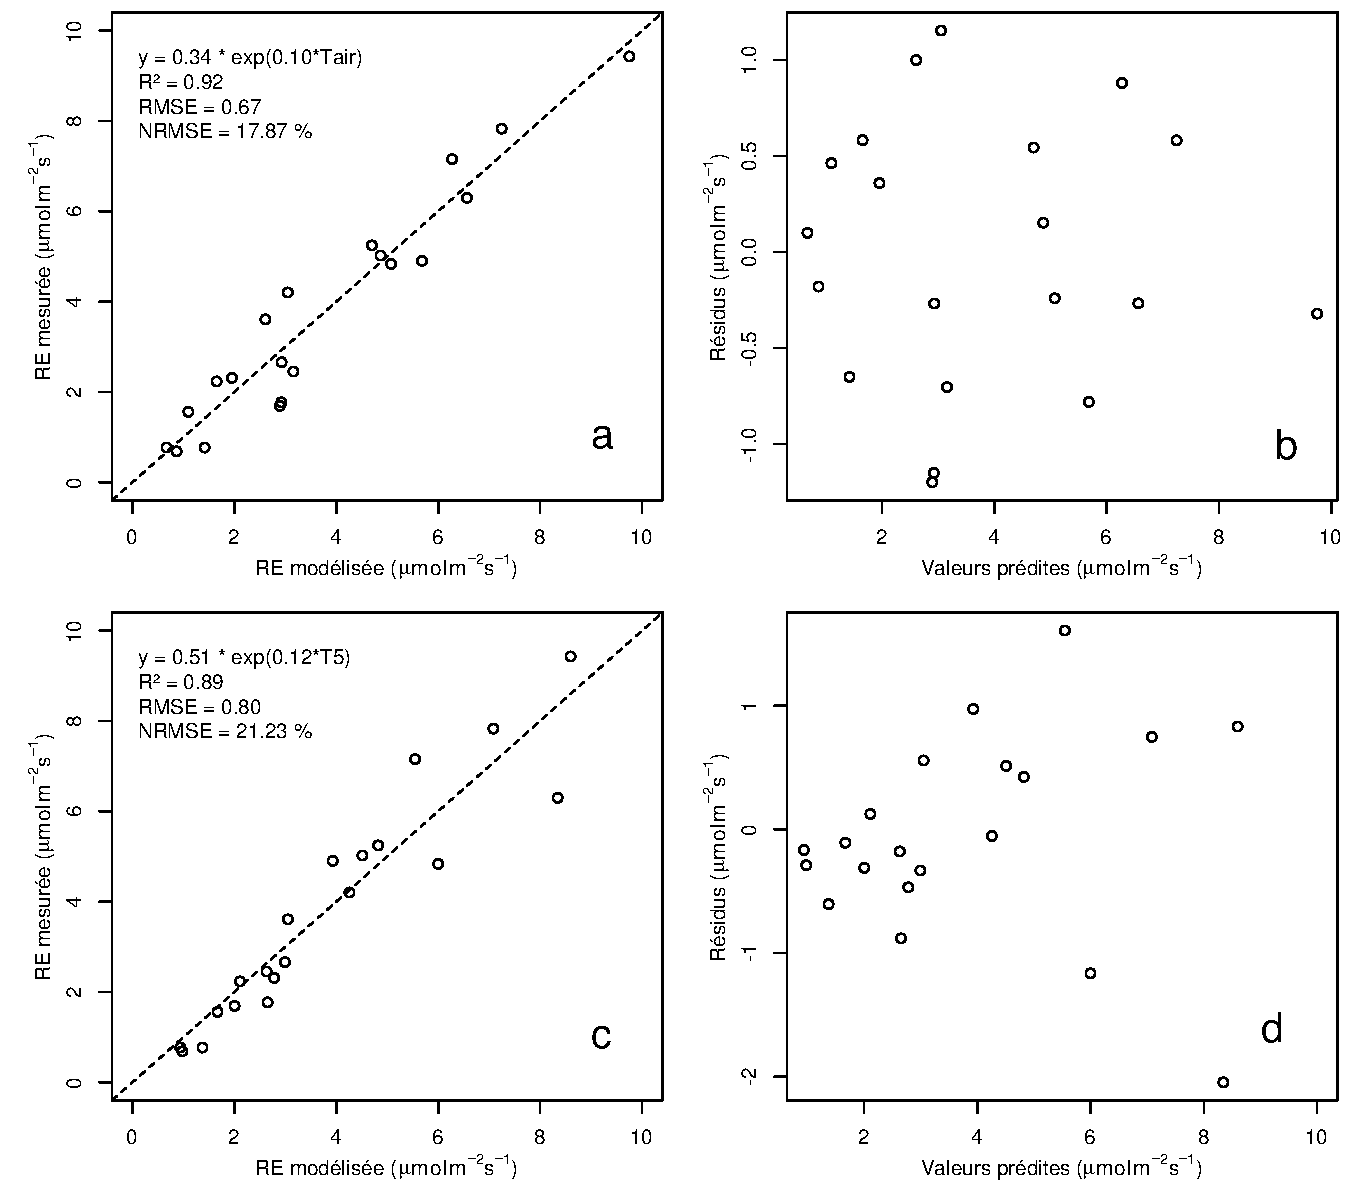
\includegraphics[width=\textwidth]{chap3/ER_mdl}
\caption{RE modèles avec T5}
\label{fig:ER_mdl}
\end{figure}

%%%%%%%%%%%%%%%%%%%%% ENE
\subsubsection{L'Échange Net de l'Écosystème}

\begin{figure}
\centering
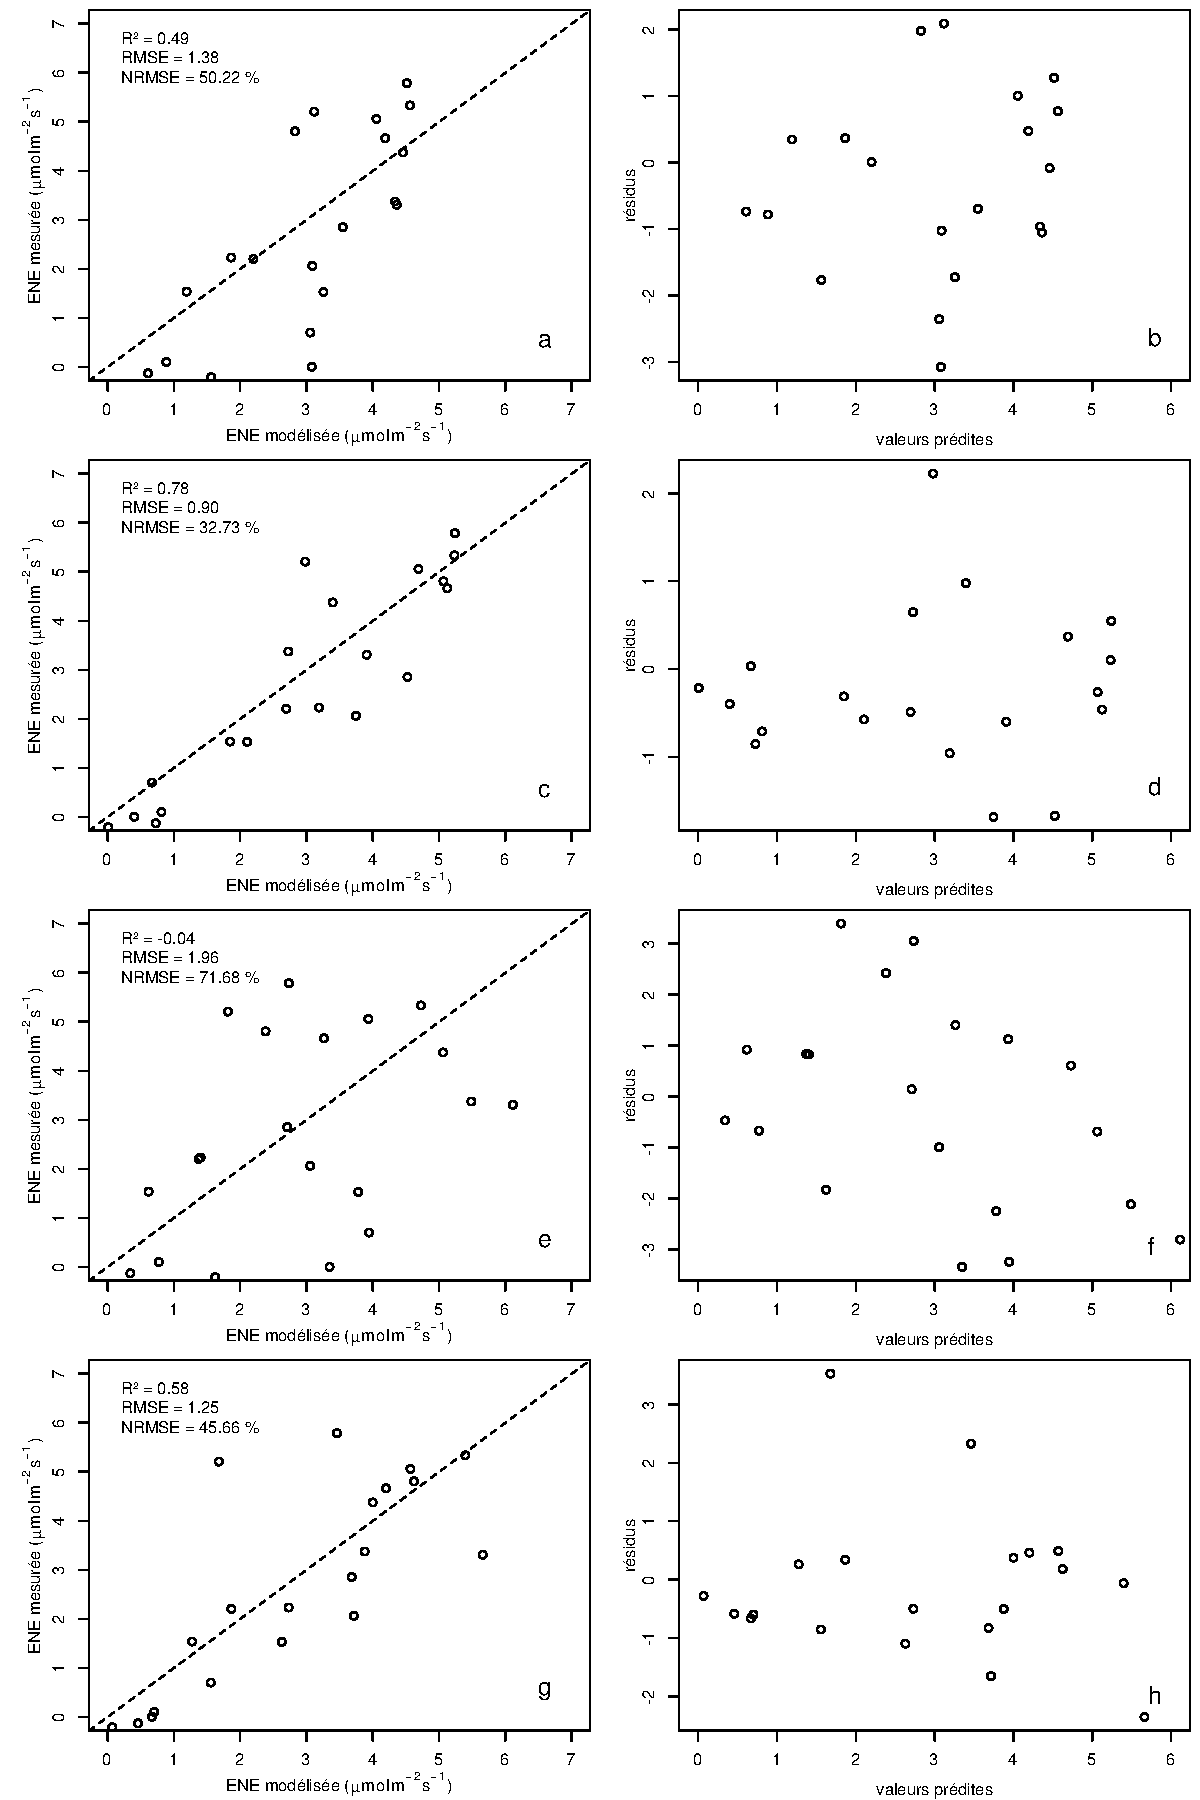
\includegraphics[width=\textwidth]{chap3/NEE_mdl_mesmod}
\caption{ENE modèle T5 IV}
\label{fig:ENE_mdl}
\end{figure}

L'ENE est ensuite modélisé en utilisant l'équation suivante :

\begin{equation}
ENE = PBB-RE
\end{equation}

Le résultat de cette équation (Figure~\ref{fig:ENE_mdl}), montre que ce modèle permet d'expliquer une grande partie des variations de l'ENE.
Les résidus de cette équation sont répartis de manière a peu près homogène.

\subsubsection{Le flux de \chh}

\begin{figure}
\centering
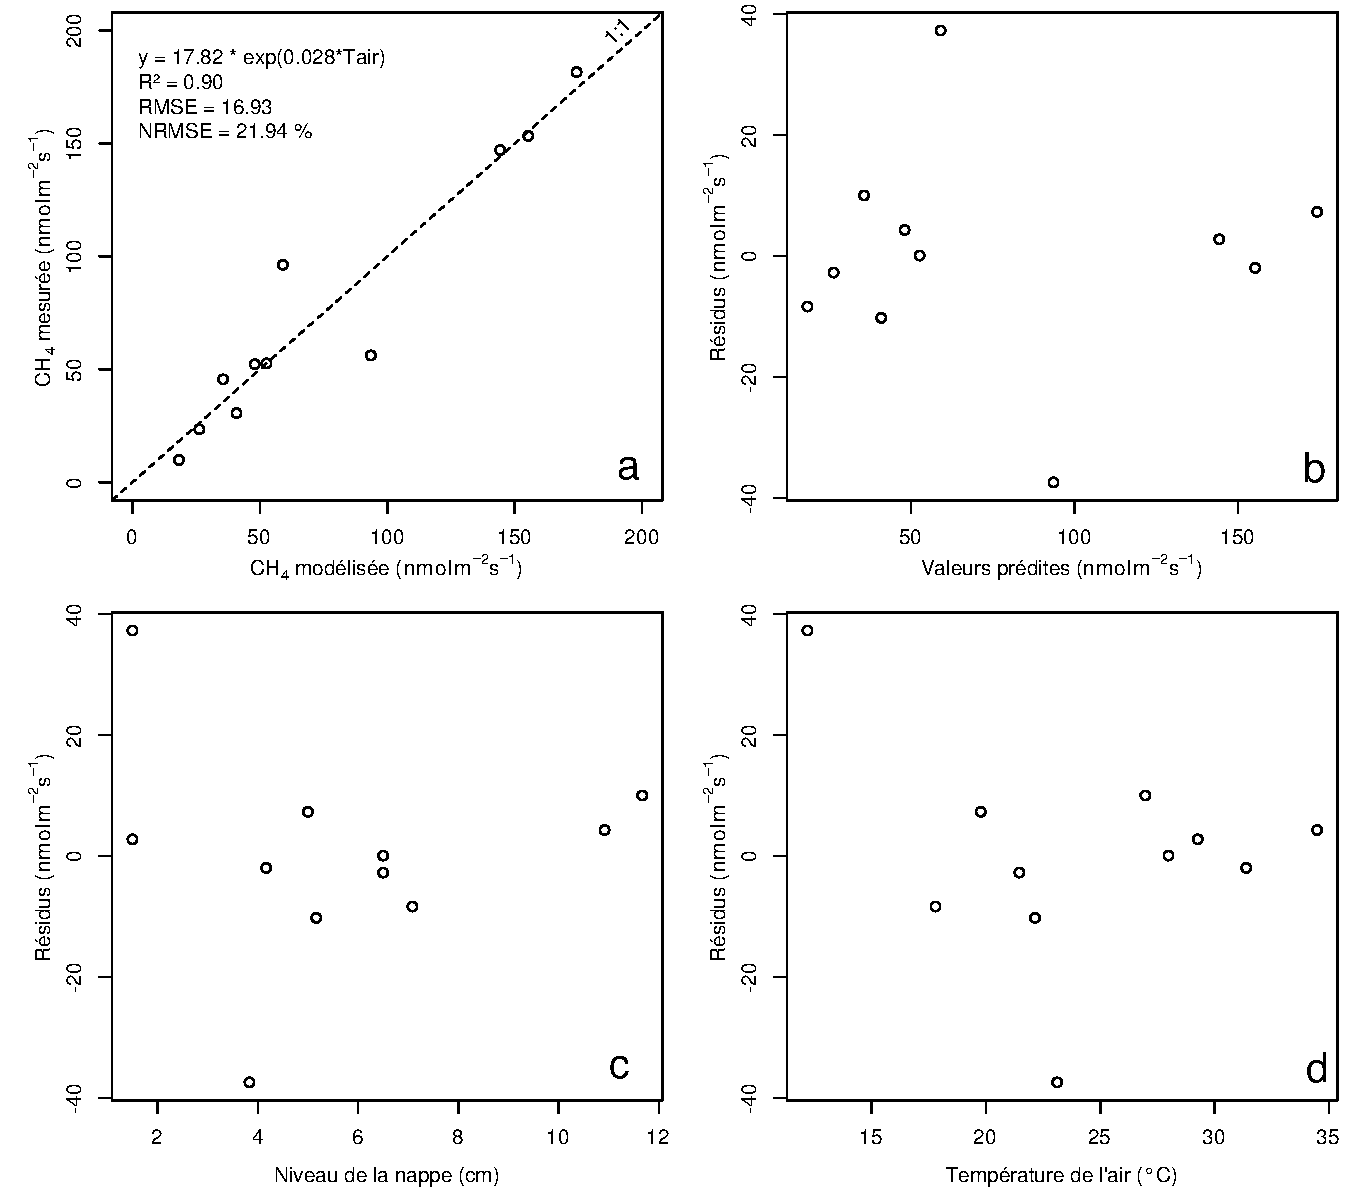
\includegraphics[width=\textwidth]{chap3/CH4_H_mdl_mesmod}
\caption{CH4 modèle H}
\label{fig:CH4_mdl}
\end{figure}

Pas de consensus clair émerge de la littérature quand aux facteurs prépondérant dans le contrôle du \chh.
La température, peut être utilisée \cite{alm1999,bubier1995}, le niveau de la nappe \cite{bubier1993} ou la végétation \cite{bortoluzzi2006}.
Avec les données acquises, le recouvrement les herbacées H est le meilleur prédicteur (Figure~\ref{fig:CH4_mdl}).
le méthane est également corrélé avec les températures, faiblement avec les température de surface puis plus fortement avec les températures du sol à plus forte profondeur.
Enfin il est anti-corrélé (R=-0.51) avec le niveau de la nappe.

%bortoluzzi veg
%Alm 1999 T -30 cm
%Bellisario relation inverse avec WTL (increased flux with lower WTL) T10
%Bubier 1993a WTL majeur
%Bubier 1995 Température humidité végétation

\subsubsection{Le COD}

\section{Résultats}

\subsection{Évolution générale des flux et facteurs contrôlants sur la tourbière de La Guette}

\subsubsection{Les Facteurs contrôlant}

\begin{figure}
\centering
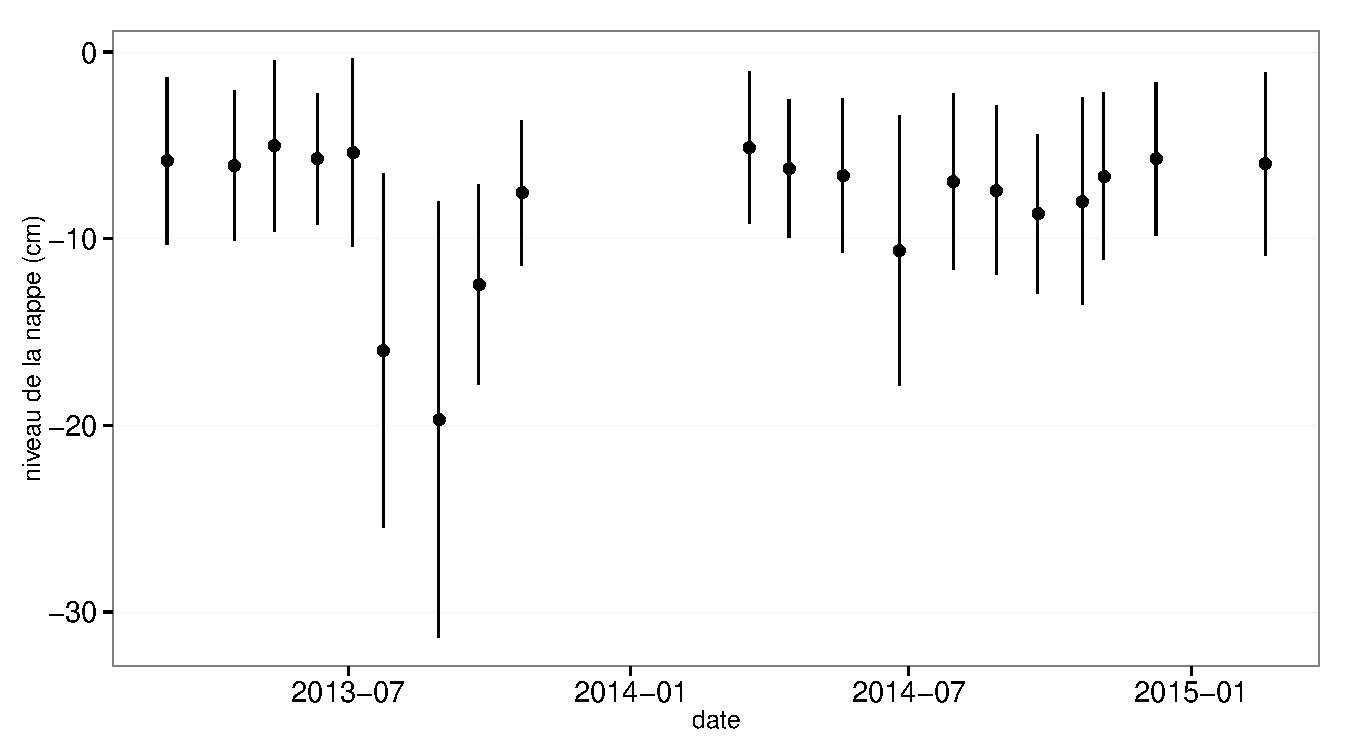
\includegraphics[width=\textwidth]{chap3/WTL_mean_evolution}
\caption{Évolution du niveau de la nappe moyen des 20 embases mesuré pendant la période de mesure (mars 2013 -- février 2015)}
\label{fig:WTL_mean_evolution}
\end{figure}

L'évolution du niveau de la nappe des 20 placettes, décrite dans la figure~\ref{fig:WTL_mean_evolution}, est marquée par un étiage d'une vingtaine de centimètres en moyenne en 2013 et l'absence d'un étiage net en 2014 avec un niveau de la nappe moyen ne descendant que rarement sous la barre des \SI{-10}{\cm}.
Ces observations sont cohérentes avec la figure~\ref{fig:WTL} représentant des données acquises à plus haute fréquence, et confirment la particularité de ces 2 années vis à vis des précédentes qui présentent des étiages bien plus fort.

\begin{figure}
\centering
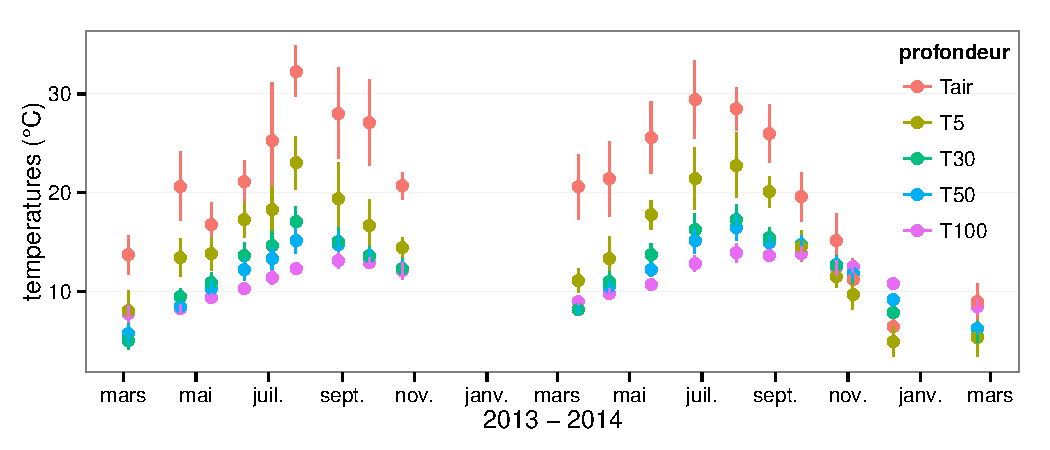
\includegraphics[width=\textwidth]{chap3/T_mean_evolution}
\caption{Évolution des températures de l'air (Tair) et du sol à \SIlist{-5;-30;-50;-100}{\centi\metre} (T5, T30, T50 et T100 respectivement) moyenne mesurée lors des campagnes de terrain de mars 2013 à février 2015}
\label{fig:T_mean_evolution}
\end{figure}

La température de l'air mesurée manuellement montre une variabilité saisonnière cohérente avec celle mesurées par la station météo. 
%bien que les valeurs semblent systématiquement supérieures.
La variabilité saisonnière de la température est également visible dans le sol avec cependant un amortissement et une diminution de la variabilité avec la profondeur (figure~\ref{fig:T_mean_evolution})
%chiffres ?

\begin{figure}
\centering
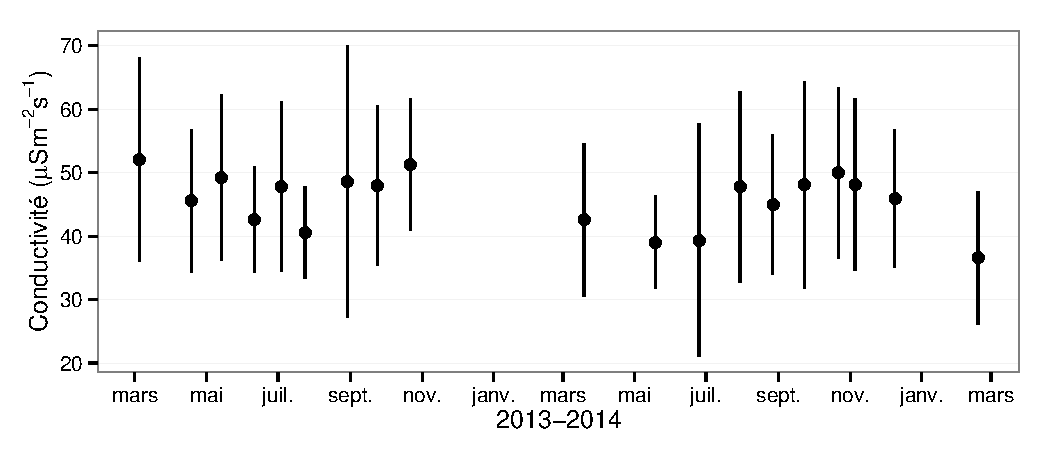
\includegraphics[width=\textwidth]{chap3/cond_mean_evolution}
\caption{Évolution de la conductivité pendant la période de mesure (mars 2013 -- février 2015)}
\label{fig:cond_mean_evolution}
\end{figure}

La conductivité moyenne mesurée sur le site varie entre \SIlist{35;55}{\usml} (figure~\ref{fig:cond_mean_evolution}).


\begin{figure}
\centering
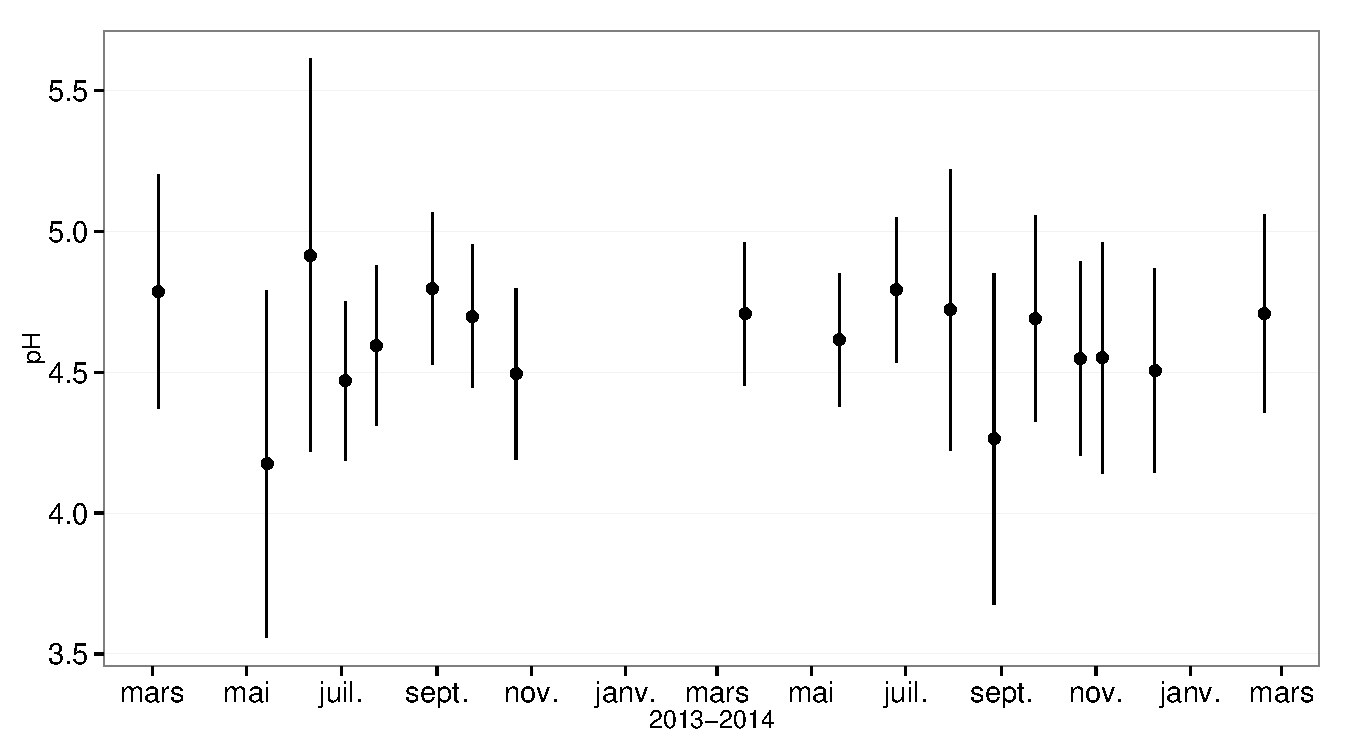
\includegraphics[width=\textwidth]{chap3/pH_mean_evolution}
\caption{Évolution du pH pendant la période de mesure (mars 2013 -- février 2015)}
\label{fig:pH_mean_evolution}
\end{figure}


En moyenne le pH mesuré sur la tourbière de La Guette est compris entre 4 et 5 (figure~\ref{fig:pH_mean_evolution}).
Ces valeurs sont cohérentes avec la classification \textit{poor-fen} du site .


\begin{figure}
\centering
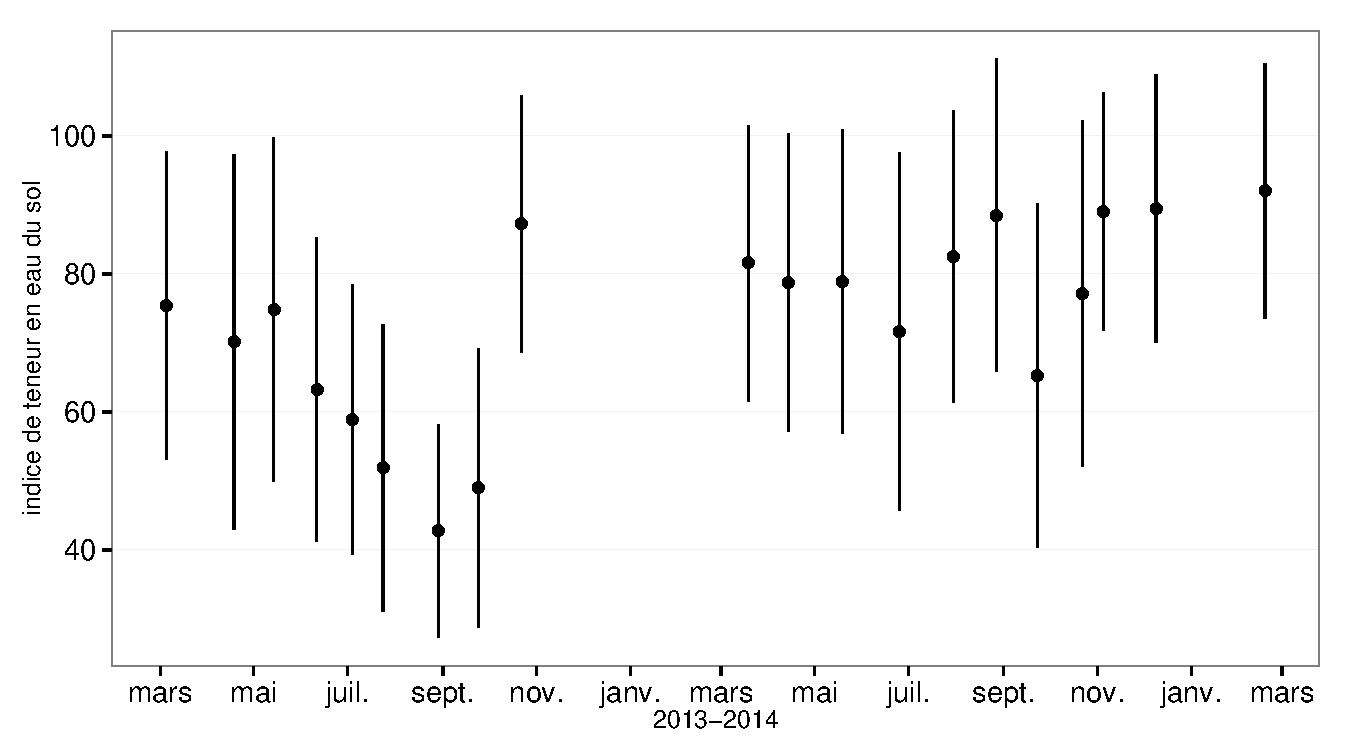
\includegraphics[width=\textwidth]{chap3/RH_mean_evolution}
\caption{Évolution de la teneur en eau du sol pendant la période de mesure (mars 2013 -- février 2015)}
\label{fig:RH_mean_evolution}
\end{figure}

\begin{figure}
\centering
\includegraphics[width=\textwidth]{chap3/NPOC_mean_evolution}
\caption{Évolution de la teneur en eau du sol pendant la période de mesure (mars 2013 -- février 2015)}
\label{fig:NPOC_mean_evolution}
\end{figure}

%\subsection{Évolution générale des flux de C sur la tourbière de La Guette}

\subsubsection{Les flux de carbone}

\begin{figure}
	\centering
	\begin{subfigure}[t]{\textwidth}
		\centering
		\includegraphics[width=\textwidth]{chap3/GPP_evolution_avg}
		\caption{Production primaire brute}
		\label{fig:GPP_evolution_avg}
	\end{subfigure}%
	
	\begin{subfigure}[t]{\textwidth}
		\centering
		\includegraphics[width=\textwidth]{chap3/ER_evolution_avg}
		\caption{Respiration de l'écosystème}
		\label{fig:ER_evolution_avg}
	\end{subfigure}
	
	\begin{subfigure}[t]{\textwidth}
		\centering
		\includegraphics[width=\textwidth]{chap3/NEE_evolution_avg}
		\caption{Échange net de l'écosystème}
		\label{fig:NEE_evolution_avg}
	\end{subfigure}
\caption{Évolution du niveau de PPB, RE et ENE pendant la période de mesure. Moyenne des 20 embases de mars 2013 à février 2015.}
\label{fig:flux_evolution_avg}
\end{figure}

%\subsubsection{PBB}
L'ensemble des mesures de \coo s'étendent de mars 2013 à février 2015.
Cependant de novembre 2013 à février 2014 les mesures ont été interrompue suite à des pannes/casses matérielles.
Malgré cela les périodes les plus critiques, notamment la saison de végétation, ont pu être mesurées pour les 2 années, permettant d'avoir une vision correcte/globale de chacune d'elle.
À noter également que pour l'ensemble des flux, la déviation standard augmente avec les valeurs mesurées.

En 2013, les valeurs de la PPB augmentent au printemps et une partie de l'été avec un maximum de \SI{999999(888)}{\uml} atteint fin juillet, avant de diminuer à partir d'août.
En 2014 le maximum de PPB, \SI{99999(888)}{\uml}, est atteint en juin, soit plus tôt que l'année précédente.
Puis pendant l'été et l'automne les valeurs décroissent jusqu'à être proche de 0.
En moyenne les valeurs de la PPB sont de \SI{7.12(519)}{\uml} en 2013 et de \SI{6.56(472)}{\uml} en 2014 (Figure~\ref{fig:GPP_evolution_avg}).

La RE en 2013 augmente pendant le printemps et une partie de l'été, elle atteint un maximum de \SI{99999(888)}{\uml} en juillet avant de diminuer.
En 2014 la RE atteint, comme la PPB, son maximum plus tôt, en juin à \SI{99999(888)}{\uml} avant de décroître jusqu'en hiver pour approcher des valeurs nulles.
La moyenne annuelle de RE en 2013 est de \SI{4.27(316)}{\uml}, ce qui est légèrement supérieure à celle de 2014 : \SI{3.63(256)}{\uml}(Figure~\ref{fig:ER_evolution_avg}).

Concernant l'ENE, en 2013 elle augmente jusqu'en juin avec un maximum à \SI{99999(888)}{\uml} avant de diminuer jusqu'à la fin de l'année.
Cependant, cette baisse est moins homogène que celle des deux flux précédents, avec notamment une augmentation de l'ENE entre juillet et août 2013.
Ceci étant, il faut également noter les valeurs importantes de la déviation standard particulièrement en juin et en août.
En 2014, l'ENE maximum est atteinte en juillet avec \SI{99999(888)}{\uml} avant qu'elle ne décroisse.
Cette baisse est cependant plus homogène qu'en 2013.
les moyennes de l'ENE en 2013 et 2014 sont très proche est sont respectivement de \SI{2.85(305)}{\uml} et \SI{2.93(277)}{\uml} (Figure~\ref{fig:NEE_evolution_avg}).

%\subsubsection{Le \chh}

Le \chh comme le \coo montre une variabilité saisonnière importante, cependant les flux mesurés sont un ordre de grandeur en dessous de ceux mesurés pour le \coo.
À l'inverse de ce dernier, l'importance des flux de \chh mesurés en 2013 et 2014 est différente.
En 2013 les flux sont moins important qu'en 2014 avec des maximum de \SIlist{0.078;0.196}{\uml} respectivement.

\begin{figure}
\centering
\includegraphics[width=\textwidth]{chap3/CH4_evolution_avg}
\caption{Évolution des flux de méthane moyen (N ?) pendant la période de mesure (mars 2013 -- février 2015)}
\label{fig:CH4_evolution_avg}
\end{figure}

%\subsubsection{Le Carbone Organique Dissous (COD)}

\subsubsection{Les relation flux gazeux et facteurs contrôlants}

\begin{figure}
\centering
\includegraphics[width=\textwidth]{chap3/Fl_FC}
\caption{Relations entre les flux de gaz et une sélection de facteurs contrôlant}
\label{fig:Fl_FC}
\end{figure}

Comme précisé précédemment, le niveau de la nappe n'a que peu varié pendant les deux années de mesures.
De ce fait aucune relation claire ne se distingue entre les flux et le niveau de la nappe que ce soit pour le \coo (PPB et RE) ou le \chh (Figure~\ref{fig:Fl_FC}).
La PPB et la RE présentent cependant des relations avec la température de l'air, et l'indice de végétation, même si pour ce dernier les tendance sont moins évidentes, particulièrement pour la RE.
Le \chh quand à lui ne présente pas de relation avec la température de l'air, mais une tendance exponentielle est visible vis à vis de l'indice de végétation.
\textbf{(\chh et Température dans la tourbe ?)}

\subsection{Le bilan de carbone de la tourbière de La Guette à l'échelle de l'écosystème}

\subsubsection{Bilan (param et valeur)}

\begin{table}
\centering
\caption{Valeur des paramètres des équations utilisées pour modéliser les flux et sensibilité relative (en \%) des flux en réponse à une variation de $\pm$\SI{10}{\percent} de chacun des paramètres des modèles.}
\label{table:mdl_par}
\begin{tabular}{llccccc}\toprule

& par & valeur & se & pval & \SI{-10}{\percent} & +\SI{+10}{\percent} \\ \midrule
%\multicolumn{7}{l}{PPB -- Tair}  \\ [+.5ex]
%& a & 26.23 & 62.07 & & -9.7 & 9.6 	\\
%& b & 53.68 & 61.27 & & 43.7 &-35.1 \\
%& c & 27.21 & 28.56 & &-22.5 & 21.9 \\
%& i &  1.84 &       & & -0.4 &  0.4 \\[+1ex]
\multicolumn{7}{l}{PPB -- Tair IV}  \\ [+.5ex]
& a & 33.66 & 19.89 & & -9.0 & 8.9 \\
& b & 42.45 & 22.28 & & 19.3 & -19.9 \\
& c & 25.77 & 15.28 & & -10.1 & 8.6 \\
& i &  0.33 &       & & -1.1 & 1.0 \\[+1ex]
\multicolumn{7}{l}{ER -- Tair}  \\ [+.5ex]
& a & 0.34 & 0.08 &  & -10 & +10 \\
& b & 0.10 & 0.01  & & -22.6 & +29.9  \\[+1ex]
%\multicolumn{7}{l}{ER -- T5}  \\ [+.5ex]
%& a & 0.51 & 0.12 & & -10 & +10 \\
%& b & 0.12 & 0.01 & & -19.4 & 24.7 \\[+1ex]
\multicolumn{7}{l}{CH4 -- IV}  \\ [+.5ex]
& a & 0.00 & 0.00 & & -10 & +10 \\
& b & 13.01 & 2.82 & & -43.9 & 79.2 \\[+1ex]
\bottomrule
\end{tabular}
\end{table}

Afin de calculer le bilan à l'aide des équations XXXX, la température de l'air mesurée au niveau de la station météo à été utilisée.
Pour l'indice de végétation, le bilan a été calculé avec une interpolation linéaire entre les points.

\begin{figure}
\centering
\begin{subfigure}{.5\textwidth}
  \centering
  \includegraphics[width=\linewidth]{chap3/ER_T5_val}
  \caption{évalutation RE}
  \label{fig:sub1}
\end{subfigure}%
\begin{subfigure}{.5\textwidth}
  \centering
  \includegraphics[width=\linewidth]{chap3/GPP_TairIVcov_val}
  \caption{évaluation PPB}
  \label{fig:sub2}
\end{subfigure}
\caption{Évaluation modèles}
\label{fig:test}
\end{figure}


\begin{table}
\centering
\caption{Bilan en gCm2an1}
\label{table:BdC}
\begin{tabular}{lllllll}\toprule
& année & PBB & RE & CH4 & COD & BCNE \\ \midrule
mdl 1 (Tair - Tair - IV) & 2013 & 1317.8 & 1332.8 & 10.1 & & \\[+.5ex]
                         & 2014 & 1257.7 & 1273.3 & 24.6 & & \\ [+1ex]
                         & total & 1287.7 & 1283.9 & 17.4 & &\\[+2ex]
%mdl 2 (Tair IV - Tair - IV) & 2013 & 1035.2 & 1332.8 & 10.1 & & \\[+.5ex]
%                            & 2014 & 1212.9 & 1273.3 & 24.6 &  & \\ [+1ex]
%                            & total & 1124.1 & 1283.9 & 17.4 & &\\[+2ex]
%mdl 3 (Tair IV - T5 - IV) & 2013 & 1035.2 & 1358.8 & 10.1 & & \\[+.5ex]
%                          & 2014 & 1212.9 & 1273.3 & 24.6 & & \\ [+1ex]
%                          & total & 1124.1 & 1288.6 & 17.4 & &\\[+1ex]
\bottomrule
\end{tabular}
\end{table}




\begin{figure}
\centering
\includegraphics[width=\textwidth]{chap3/BdC_interp}
\caption{Flux de \coo interpolé à partir des équations~\ref{eq:juneTairIV} et \ref{eq:PPB_bubier} pour la GPP et de l'équation~\ref{eq:RE_T} pour RE.}
\label{fig:BdC_interp}
\end{figure}






\subsubsection{Évaluation du bilan}

%\subsubsection{sensibilité des paramètres}

L'analyse de sensibilité, consistant à faire varier chaque paramètre des modèles de $\pm$\SI{10}{\percent}, montre pour une équation exponentielle simple des valeurs attendues $\pm$\SI{10}{\percent} pour le paramètre a et \num{+29} à \SI{-22}{\percent} pour le b (Figure~\ref{table:mdl_sensitiv}).
Pour la PPB issue des équations~\ref{eq:juneTairIV} et \ref{eq:PPB_bubier} le paramètre i à très peu d'effet sur le bilan, \num{0} à \SI{-1}{\percent}.
Cependant l'effet sur le bilan augmente lorsque la végétation est prise en compte (équation~\ref{eq:juneTair} et \ref{eq:PPB_bubier}) : \num{-8} à \SI{-10}{\percent}.
À l'inverse, la sensibilité de l'ensemble des autres paramètres (a, b, c) diminue lorsque l'indice de végétation est pris en compte.
Le paramètre a est l'exception, passant de \num{-10} à \SI{-17}{\percent} pour une baisse de \SI{10}{\percent}.
Considérant le modèle de PPB prenant en compte la végétation, la sensibilité maximum des différents paramètres du bilan est proche de \SI{30}{\percent}, et similaire pour la PPB et la RE.

\begin{table}
\centering
\caption{Sensibilité relative (en \%) du bilan de \coo (ENE) en réponse à une variation de $\pm$\SI{10}{\percent} de chacun des paramètres des modèles.}
\label{table:mdl_sensitiv_BdC}
\begin{tabular}{llccccccccccc}\toprule
& \multicolumn{4}{l}{RE} & \multicolumn{4}{l}{GPP} & \multicolumn{4}{l}{\chh} \\ 
& par & valeur & \SI{-10}{\percent} & +\SI{+10}{\percent} & par & valeur & \SI{-10}{\percent} & +\SI{+10}{\percent} & par & valeur & \SI{-10}{\percent} & +\SI{+10}{\percent} \\ \midrule
\multicolumn{13}{l}{mdl 1 équation~\ref{eq:RE_T5} et équation~\ref{eq:juneTair} Tair, Tair, H} \\ [+.5ex]
& a & 0.34 & -766 & 766 & a & 26.23 & 741 & -736 & a & 17.82 & -12.28 & 12.28 \\
& b & 0.10 & -1730 & 2289 & b & 53.68 & -3358 & 2693 & b & 0.03 & -15.08 & 17.68 \\
&  &  & & & c & 27.21 & 1725 & -1680 & & & & \\
&  &  & & & i & 1.84 & 31.56 & -26.92 & & & & \\[+1ex]
\multicolumn{13}{l}{mdl 2 équation~\ref{eq:RE_T5} et équation~\ref{eq:juneTairIV} Tair, Tair IVcov, H} \\ [+.5ex]
& a & 0.34 & -71.08 & 71.08 & a & 33.66 & 56.25 & -55.32 & a & 17.82 & -1.14 & 1.14 \\
& b & 0.10 & -160.59 & 212.51 & b & 42.45 & -119.84 & 123.69 & b & 0.03 & -1.40 & 1.64 \\
&  &  & & & c & 25.77 & 62.63 & -53.28 & & & & \\
&  &  & & & i & 0.33 & 6.94 & -6.02 & & & & \\[+1ex]
\multicolumn{13}{l}{mdl 3 équation~\ref{eq:RE_T5IV} et équation~\ref{eq:juneTairIV} Tair IVcov, Tair IVcov, H} \\ [+.5ex]
& a & 0.92 & -55.69 & 55.69 & a & 33.66 & 61.31 & -60.31 & a & 17.82 & -1.24 & 1.24 \\
& b & 0.09 & -149.40 & 189.01 & b & 42.45 & -130.64 & 134.84 & b & 0.03 & -1.53 & 1.79 \\
& c & 0.14 & -20.89 & 20.89 & c & 25.77 & 68.28 & -58.08 & & & & \\
&  &  & & & i & 0.33 & 7.57 & -6.56 & & & & \\
\bottomrule
\end{tabular}
\end{table}


%\begin{table}
%\centering
%\caption{Sensibilité relative (en \%) des flux en réponse à une variation de $\pm$\SI{10}{\percent} de chacun des paramètres des modèles.}
%\label{table:mdl_sensitiv}
%\begin{tabular}{llccccccccccc}\toprule
%& \multicolumn{4}{l}{RE} & \multicolumn{4}{l}{GPP} & \multicolumn{4}{l}{\chh} \\ 
%& par & valeur & \SI{-10}{\percent} & +\SI{+10}{\percent} & par & valeur & \SI{-10}{\percent} & +\SI{+10}{\percent} & par & valeur & \SI{-10}{\percent} & +\SI{+10}{\percent} \\ \midrule
% & \multicolumn{4}{l}{Tair} & \multicolumn{4}{l}{Tair} & \multicolumn{4}{l}{H} \\ [+.5ex]
%& a & 0.34 & -10   & 10   & a & 26.23 & -9.7 &  9.6 & a & 17.82 &-10.0 & 10.0 \\
%& b & 0.10 & -22.6 & 29.9 & b & 53.68 & 43.7 &-35.1 & b &  0.03 &-12.3 & 14.4 \\
%&   &      &       &      & c & 27.21 &-22.5 & 21.9 &   &       &      &      \\
%&   &      &       &      & i &  1.84 & -0.4 &  0.4 &   &       &      &      \\[+1ex]
% & \multicolumn{4}{l}{Tair IVcov} & \multicolumn{4}{l}{Tair IVcov} & & & & \\ [+.5ex]
%& a & 0.92 & -7.3  & 7.3 & a & 33.66 & -9.0 &  8.9 & & & & \\
%& b & 0.09 & -19.5 & 24.7& b & 42.45 & 19.3 &-19.9 & & & & \\
%& c & 0.14 & -2.7  & 2.7 & c & 25.77 &-10.1 &  8.6 & & & & \\
%&   &      &       &     & i & 0.33  & -1.1 &  1.0 & & & & \\[+1ex]
%\bottomrule
%\end{tabular}
%\end{table}




%\subsubsection{pseudo-validation et erreur}

%\begin{figure}
%\centering
%\includegraphics[width=.5\textwidth]{chap3/ER_T5_val}
%\caption{Évaluation RE}
%\label{fig:RE_T5_val}
%\end{figure}
%\begin{figure}
%\centering
%\includegraphics[width=.5\textwidth]{chap3/GPP_TairIVcov_val}
%\caption{Évaluation GPP}
%\label{fig:GPP_TairIVcov_val}
%\end{figure}

\subsection{Variabilité spatiale du bilan}

\subsubsection{Représentativité locale}

\subsubsection{Modélisation par placette}

\subsubsection{Corrélation avec facteurs contrôlant}

\section{Discussion}

\subsection{Représentativité du modèle à l'échelle de l'écosystème}

Valeur absolue des flux

Différence entre 2013 et 2014

apport d'un indice de végétation

\subsection{Sensibilité et limitations du bilan}

sensibilité du bilan au variation des paramètres

limitations

\begin{itemize}
\item pas d'arbres
\item pas de zones à gros touradons
\item pas de cartographie (mais pas grave si les placette sont maj bien représentée par mdl ecos)
\item extrapolation sur d'autres site difficile (cf validation)
\end{itemize}

\subsection{Représentativité locale du modèle}

Distribution des paramètres

Pourquoi certaines placette mieux que d'autres




 %Bilan de C de la tourbière de La Guette
% CHAPITRE 4
\singlespacing
\chapter{Effets de l'hydrologie sur les flux de GES}
\label{ch:4}

\minitoc

\newpage
\doublespacing
%\section{Manipulation du niveau de l'eau en mésocosmes}
\section{Introduction}

Au cours des deux années de suivis des flux de \coo et de \chh sur la tourbière de La Guette, le niveau de la nappe a très faiblement varié comparé aux années précédentes bien plus sèches.
En conséquence l'effet des variations de nappe sur les flux n'a pu être investigué.
% de cette faible variation peu de variations des flux ont pu y être relié.
Néanmoins l'hydrologie est un facteur contrôlant des flux \plop.
Ainsi de nombreuses études ont reliées les émissions de \coo au niveau de la nappe \plop.
Cependant, aucun consensus n'a encore été atteint :
La majorité des études montrent qu'une tourbière dont le niveau de la nappe est abaissé, soit par un drainage, soit par une sécheresse, aura tendance à avoir un ENE plus faible.
Par exemple, \citet{strack2013} expliquent des valeurs d'ENE plus faibles qu'escompté, par des mesures faites pendant une période relativement sèche.
Une observation similaire est faite par \citet{aurela2007} qui mesure un ENE plus faible lors d'une année sèche, sur une tourbière à Carex du sud de la Finlande.
Ils attribuent la variation de l'ENE à une augmentation de la RE et à une baisse de la PPB, dans des conditions plus chaudes et plus sèches.
\citet{peichl2014} observent également une baisse de l'ENE lors d'une année ou le niveau de la nappe baisse de façon importante, au delà de \SI{-30}{\centi\metre}.
Ils expliquent cette baisse par une baisse de la PPB.
Cette observation va dans le même sens que \citet{lund2012} qui observent en 2008 une baisse de l'ENE sur une tourbière à sphaignes située au sud de la suède.
% dont la végétation, Calluna vulgaris, Erica tetralix, Eriophorum vaginatum
Les mesures de RE faites cette année là étant similaires à celles effectuées les autres années, ils lient cette baisse à une diminution de la PPB.
En 2006, sur la même tourbière, \citet{lund2012} observent une autre baisse de l'ENE.
Mais cette fois, les mesures de PPB à leur tour similaires à celle des autres années n'expliquent pas cette baisse.
À l'inverse de 2008, cette baisse est expliqué par une augmentation de la RE.
Ces inconsistances apparentes peuvent avoir pour origine des types de sécheresse différente : courte et intense pendant la saison de végétation de 2006 et d'intensité plus faible mais d'une durée plus longue en 2008.
À l'inverse des résultats précédemment cités, \citet{ballantyne2014} dans une étude des effets à long terme d'une baisse du niveau de la nappe, observent pas d'effets significatifs sur l'ENE tandis que les flux de RE et de PPB augmentent tous les deux.
Ces études montrent que si le niveau de la nappe est reconnu comme un facteur de contrôle des flux de \coo, il est difficile d'en dégager des liens de cause à effet répétables.

Concernant le méthane, une baisse du niveau de la nappe est généralement liée à une baisse des émissions de \chh, et inversement, le niveau de la nappe contrôlant la proportion des zones ou le \chh est produit/oxydé \citep{pelletier2007}.
\citet{turetsky2008} montrent par ailleurs que selon leur sens, l'effet des variations du niveau de nappe sur les flux de \chh n'est pas identique.
Ils observent ainsi que l'effet est plus important lorsque le niveau de la nappe est augmenté que lorsqu'il est diminué ($\pm$ \SI{10}{\centi\metre}).
Ils font l'hypothèse que le niveau de la nappe, en plus de jouer sur la proportion production/oxydation, a un effet sur le transfert de chaleur dans le sol.
Cette hypothèse s'appuie sur l'observation de températures plus élevées, que ce soit celles de l'air ou de la tourbe, dans les zones ou le niveau de la nappe a été rehaussé.
Cependant d'autres études, principalement dans des sites ou le niveau de la nappe est proche de la surface du sol, montrent une absence de relation entre le niveau de la nappe et les émissions de méthane, voire une relation inverse, avec des flux plus faibles liés à des niveaux de nappe plus élevés \citep{kettunen1996,bellisario1999,treat2007}.
Là encore selon les conditions environnementales, la relation entre les flux de \chh et le niveau de la nappe n'est pas aisément généralisable.

La vitesse de l'augmentation du niveau de nappe semble également jouer sur les flux, des pics de RE ont été observés après la réhumectation rapide 
La façon dont le niveau de la nappe augmente semble également jouer sur les flux.
\citet{strack2009} ont observés qu'une hausse graduelle par le bas de la colonne de sol conduit à une baisse de la RE, tandis qu'une hausse rapide simulant un événement pluvieux (par le haut) conduisait à un pic de RE.
Ce pic de RE après une réhumectation a également été observé par \citet{mcneil2003}.
L'objectif de ce chapitre est donc d'explorer plus en avant l'effet du niveau de la nappe d'eau sur les émissions de GES, effet peu ou pas visible \textit{in-situ}.
Plus précisément il s'agit de déterminer l'effet de cycles de dessication/ré-humectation sur les émissions de \coo et de \chh. 
%\citet{treat2007} montre également que selon l'échelle de temps le niveau de la nappe peut être corrélé soit négativement, soit positivement avec les flux de \chh.

\section{Procédure expérimentale}

L'étude des cycles de dessication/ré-humectation est effectuée sur des mésocosmes, prélevés à la tourbière de La Guette.
L'expérimentation a été réalisée durant l'été 2013 avec un seul cycle relativement long, on s'y référera par la suite comme l'expérimentation A.
L'expérimentation a été renouvelée l'été 2014 avec trois cycles, plus courts.
On appellera cette seconde expérimentation, l'expérimentation B (Tableau~\ref{table:recap_hm}).

\subsection{Expérimentation A}
Six mésocosmes ont été prélevés le 12 avril 2013, sur la tourbière de La Guette.
Le prélèvement s'effectue à l'aide de cylindres de PVC qui, dans un premier temps, posé sur le sol, permettent de faire un pré-découpage au couteau, puis dans un second temps sont insérés, délicatement, dans la tourbe. 
Les mésocosmes sont finalement dégagés en creusant de chaque côté (Figure~\ref{fig:mesophoto}).
Les mésocosmes sont transportés au laboratoire ou ils sont enterrés en extérieur et saturé en eau (eau prélevée dans la tourbière), afin que leur conditions hydrologique de départ soient les plus proche possible (Figure~\ref{fig:mesocarte}).
Trois mésocosmes tirés au sort servent de contrôle, et trois vont subir un cycle de dessication/ré-humectation.
%À partir du 31 mars 2013 de l'eau a été pompé régulièrement dans les 3 mésocosmes traités pour simuler une sécheresse, jusqu'au 17 juillet.
À partir du 31 mars 2013 les précipitations ont été interceptées à l'aide d'abri bâchés installable en cas de pluie et la nuit.
Ces interceptions ont été faites jusqu'au 17 juillet dans les 3 mésocosmes traités pour simuler une sécheresse.
À cette date de l'eau est ajouté aux mésocosmes, que ce soit les contrôles ou les traitements, pour simuler de fortes précipitations.

\subsection{Expérimentation B}
Le 17 avril 2014, six nouveaux mésocosmes ont été prélevés sur la tourbières de La Guette et installés près du laboratoire, en suivant le même protocole que pour l'expérimentation A.
Une station météo a été installée à côté des mésocosmes afin de mesurer la température de l'air, l'humidité relative, le rayonnement solaire, la vitesse et la direction du vent et les précipitations toutes les 15 minutes.
Cette station permettait également l'enregistrement des températures mesurées par des sondes (T107) installées à \num{-5}, \num{-10}, et \SI{-20}{\centi\metre}.
Les conditions météorologiques moins ensoleillée qu'en 2013 et l'objectif de suivre plusieurs cycles de dessiccation/réhumectation ont nécessité la mise en place d'un abaissement manuel du niveau de la nappe.
Pendant les phases d'assèchement les niveaux de nappes des placettes traitées étaient donc abaissés en moyenne de \SI{2.5}{\centi\metre} par jour.
Le premier cycle de dessication/réhumectation dura du 30 juin au 6 juillet pour la phase de dessication est du 7 au 16 juillet pour la phase de réhumectation.
Le deuxième cycle dura du 17 au 28 juillet et du 29 juillet au 3 aout, 
Enfin le dernier cycle fut mesuré du 4 au 11 aout pour la dessication et du 12 au 14 aout pour la réhumectation.

\subsection{traitement}
Les flux sont moyennés par jour de mesure.

\begin{figure}
\centering
\includegraphics[width=\textwidth]{chap4/mesocosmes}\\
\includegraphics[width=\textwidth]{chap4/zi_exp_low}
\caption{Prélèvement des mésocosmes (en haut). Mésocosmes installés et protégés de la pluie (en bas).}
\label{fig:mesophoto}
\end{figure}


%\begin{table}
%\centering
%\caption{Récapitulatif des mesures pour les deux expérimentations}
%\label{table:recap_hm}
%\begin{tabular}{lll}\toprule
%expérimentation & A & B \\ \midrule
%année & 2013 & 2014 \\
%réplicats & 6 & 6 \\
%cycles & 1 & 3 \\
%station météo & non & oui\\
%\bottomrule
%\end{tabular}
%\end{table}


\begin{figure}
\centering
\includegraphics[width=.6\textwidth]{chap4/installation}
\caption{Schéma d'un mésocosme}
\label{fig:mesocarte}
\end{figure}

\section{Résultats}

\subsection{Expérimentation A}

\textbf{Niveau de la nappe}

Pendant la phase de dessication de l'expérimentation A, on observe une baisse du niveau de la nappe pour les placettes contrôles comme pour les placettes traitements (Figure~\ref{fig:HMzi}--A).
Cependant les placettes contrôles ont un niveau de nappe relativement élevé jusqu'au 24 juin puis ce niveau baisse fortement alors que les placettes du groupe traité ont un niveau de nappe qui diminue de façon plus continue sur l'ensemble de la phase.
La remontée du niveau de la nappe s'effectue de façon similaire pour les deux groupes.
Enfin après la phase de ré-humectation, le niveau de la nappe baisse à nouveau, plus rapidement pour le groupe traitement que pour le groupe contrôle.


\begin{figure}
\centering
\includegraphics[width=1.15\textwidth, center]{chap4/expA_flux}
\caption{Expérimentation A : Moyenne journalière du niveau de nappe en cm (A), et des flux, \chh, RE, PPB, ENE en \si{\uml}, B, C, D, E. Les cadres et bandes colorées correspondent à la phase de dessiccation (D) en rouge et à la phase de réhumectation (R) en bleu.}
\label{fig:HMzi}
\end{figure}

\textbf{Flux de \chh}

Les émissions de \chh, varient de 0 et \SI{0.3}{\uml}.
Elles sont similaires entre les deux groupes jusqu'au 24 juin 2013, date à partir de laquelle elles divergent (Figure~\ref{fig:HMzi}--B).
À cette date les émissions du groupe contrôle augmentent rapidement pour atteindre \SI{0.55(031)}{\uml} tandis que celles du groupe traité restent stable.
À la fin de la phase de dessiccation, mi-juillet, les deux groupes retrouvent des niveaux d'émission similaires compris entre \num{0.1} et \SI{0.2}{\uml}.
Ces niveaux restent constant pendant toute la phase de réhumectation, avant d'augmenter légèrement par la suite pour se situer entre \SI{0.25}{\uml} et \SI{0.2}{\uml}.

\textbf{Flux de \coo}

Pendant la phase de dessication, les valeurs de la RE tendent à augmenter quel que soit le groupe de placettes considéré (Figure~\ref{fig:HMzi}--C).
Ces valeurs inférieures à \SI{2.5}{\uml} début juin, atteignent environ \SI{7}{\uml} pour les deux groupes mi-juillet, avant la réhumectation.
Cependant la RE du groupe traité augmente régulièrement pendant l'ensemble de cette phase jusqu'à \SI{3.26(046)}{\uml} , tandis que les valeurs du groupe contrôle restent, dans un premier temps, stable jusque fin juin (\SI{2.45(075)}{\uml}).
%La RE de ce groupe vaut alors \SI{2.45(075)}{\uml} contre \SI{3.26(046)}{\uml} pour le groupe traité.
%Cet écart, pouvant varier dans le temps,  étant installé depuis le 9 juin
À partir de début juillet, les valeurs de RE du groupe de contrôle augmentent fortement dépassant les valeurs du groupe traité.
La Re de ce groupe atteint un maximum à \SI{7.93(152)}{\uml} le 8 juillet avant de retrouver des valeurs proche de celles observées dans le groupe traité.
Cette augmentation brusque correspond temporellement à celle observé, pour le même groupe, dans les flux de \chh.
Lors de la phase de réhumectation, les flux de RE diminuent de façon très similaire pour les deux groupes pour atteindre \SI{2.75}{\uml} en juin.
Ce minimum reste cependant plus élevé que les valeurs mesurées initialement.
Après la phase de réhumectation, les flux des deux groupe restent relativement proches pendant le reste des mesures, où ils remontent à mesure que le niveau de la nappe diminue à nouveau.

Pour les deux groupes, les flux de PPB restent stables pendant la phase de dessiccation (Figure~\ref{fig:HMzi}--D) :
entre 5 et \SI{6}{\uml} (\SI{5.29(076)}{\uml} de moyenne pour les deux groupes) jusqu'au 24 juin.
Ensuite comme pour le \chh et la RE, les valeurs de la PPB du groupe de contrôle augmentent et s'écartent de celles mesurées dans le groupe traité,
À la fin de cette phase de dessiccation les flux redeviennent identiques entre les traitements.
Par ailleurs, à la fin de cette phase, les flux diminuent légèrement atteignant un minimum proche de \SI{3}{\uml}.
Pendant la phase de réhumectation, la PPB augmente légèrement pour les deux groupes.
La PPB dans le groupe de contrôle a des valeurs supérieures à celles du groupe traité.
Après la réhumectation, la PPB augmente pour les deux groupes, avec un maximum de \SI{5.83(161)}{\uml} pour le groupe dessiccation et de \SI{10.17(330)}{\uml} pour le groupe contrôle.


L'ENE est systématiquement supérieure pour le groupe contrôle, avec une cinétique parallèle des flux pour les deux groupes (Figure~\ref{fig:HMzi}--E).
Pendant la phase de dessiccation, l'ENE reste relativement constante jusque fin juin avec une valeur moyenne pour les deux groupes de \SI{1.18(058)}{\uml}.
L'écart entre le groupe contrôle et le groupe traitement tend à augmenter du 10 au 30 juin environ, avant que les valeurs du groupe de contrôle ne rejoignent celles du groupe traité.
Au delà du 24 juin, l'ENE baisse fortement pour les deux groupes pour atteindre un minimum proche de \SI{-4.5}{\uml}.
Pendant la phase de réhumectation l'ENE monte rapidement pour atteindre \num{1.52(036)} et \SI{2.15(147)}{\uml} pour le groupe de contrôle et de groupe traité respectivement.
Après la réhumectation, l'ENE du groupe contrôle varie en suivant généralement les variations du niveau de nappe.
Pour le groupe traité, l'ENE baisse par rapport au maximum atteint lors de la réhumectation puis se stabilise autour de 0.

L'effet des variations du niveau de la nappe sur la PPB est quasiment nul (Figure~\ref{fig:hm_wtl}--E), même si la PPB semble diminuer aux plus fortes profondeurs.
Les variations de la RE sont principalement liée au niveau de la nappe (Figure~\ref{fig:hm_wtl}--C) Par conséquent, les variation de RE se répercutent sur l'ENE (Figure~\ref{fig:hm_wtl}--G).
Pour le \chh il est également difficile de distinguer des tendances générales entre les flux et les niveaux de nappe (Figure~\ref{fig:hm_wtl}--A).

\begin{figure}
\centering
\includegraphics[width=1.15\textwidth, center]{chap4/expB_flux}
\caption{Expérimentation B : Moyenne journalière du niveau de nappe en cm (A), et des flux, \chh, RE, PPB, ENE en \si{\uml}, B, C, D, E. Les cadres et bandes colorées correspondent aux phases de dessiccation (D) en rouge et aux phases de réhumectation (R) en bleu.}
\label{fig:HMty}
\end{figure}

\subsection{Expérimentation B}

Contrairement à l'expérimentation A, le niveau de nappe du groupe de contrôle de l'expérimentation B reste relativement constant pendant l'ensemble de la période de mesure.
Le drainage artificiel du groupe traité permet d'abaisser le niveau de la nappe d'une quinzaine de centimètres en moyenne pour chaque cycle (Figure~\ref{fig:HMty}--A).

%À l'exception du point mesuré lors de la première phase de dessiccation, les valeurs du groupe de contrôle sont systématiquement supérieures à celles du groupe traité.
Les flux de \chh moyen varient entre \num{0.07} à \SI{0.34}{\uml}.
Les flux du groupe de contrôle, à l'exception de la première mesure, sont supérieurs aux flux du groupe traité, (moyennes globales de \num{0.20(006)} et \SI{0.11(005)}{\uml}, respectivement.
Les émissions du groupe de contrôle tendent à augmenter sur la période de mesure.
Une tendance similaire, est également visible pour le groupe traité.
Concernant les cycles de dessiccation/réhumectation, il est difficile de dégager des comportements communs entre eux, même si l'assèchement conduit à une baisse des émissions (Figure~\ref{fig:HMty}--B)
Cette relation, mise en exergue pas un nombre de points très faible, n’apparaît cependant pas sur l'ensemble des données (Figure~\ref{fig:hm_wtl}--B).
Un pic d'émission de \chh est également à noter pour chaque cycle pendant la phase de dessiccation.

La RE varie pour les deux groupes entre \num{0.42} et \SI{5.12}{\uml} (Figure~\ref{fig:HMty}--C)).
Avant le démarrage des manipulations du niveau de la nappe, les valeurs des deux groupes sont très proches et augmentent tandis que le niveau de nappe diminue.
Pendant les phases de dessication, les valeurs du groupe traité sont systématiquement supérieures, de \num{1.5} à \SI{1.8}{\uml}en moyenne par phase, par rapport à celle du groupe de contrôle.
À l'inverse pendant les phases de réhumectation les flux entre les deux groupes sont beaucoup plus proches avec une tendance de la RE du groupe de contrôle à être supérieure à celle du groupe traité.
La RE du groupe traité est systématiquement plus faible pendant les phases de réhumectations que pendant les phases de dessiccations.
En moyenne la RE vaut respectivement \num{2.28(100)} et \SI{3.86(080)}{\uml} pour les groupes de contrôle et traité pendant les phases de dessiccation et \num{1.70(062)} et \SI{1.51(098)}{\uml} pendant les phases de réhumectation.
%Avant le début des traitement d'assèchement, les flux de la RE sont proches pour les deux groupes tandis qu'après, leurs comportements diffèrent (Figure~\ref{fig:HMty}--C)).
%Pendant les phases de dessiccation la RE du groupe traité est supérieure à celle du groupe de contrôle.
%La relation semble s'inverser pendant les phases de réhumectation, du moins pour les cycles 1 et 3, car pendant la phase de réhumectation du cycle 2 les deux groupes ont des valeurs similaires.

Sur l'ensemble de la période de mesure la PPB est comprise entre \num{2.78} et \SI{7.96}{\uml}.
Avant le début des traitements les flux des deux groupes sont similaires (Figure~\ref{fig:HMty}--D).
À partir de la première phase de dessiccation, la PPB du groupe de contrôle supérieure à celle du groupe traité.
Pour les deux groupes, la PPB est plus importante lors des phases de dessiccation comparée aux phase de réhumectation, avec des moyennes respectives de \num{6.35(219)} contre \num{5.80(220)} pour le groupe de contrôle et de \num{5.95(146)} contre \SI{4.05(160)}{\uml} pour le groupe traité.

Les valeurs d'ENE mesurées sont comprises entre \num{0.11} et \SI{5.42}{\uml}, elles ont tendance à augmenter au cours du temps.
Passé la période pré-traitements pendant laquelle les flux de l'ENE sont similaires pour les deux groupes l'ENE du groupe de contrôle est systématiquement supérieure à celle du groupe de traitement (Figure~\ref{fig:HMty}--E).
%Le premier cycle de dessiccation/réhumectation divise les deux groupes : le groupe de contrôle ayant des valeurs d'ENE plus élevées que celles du groupe traité.
L'évolution des deux groupes reste cependant relativement conjointe pendant la période de mesure avec pour le groupe traité une diminution récurrente de l'ENE au début de chaque phase de dessiccation.

\begin{figure}
\centering
\begin{minipage}{.5\textwidth}
\centering
\includegraphics[width=\linewidth]{chap4/expA_fluxWTL}
\end{minipage}%
\begin{minipage}{.5\textwidth}
\centering
\includegraphics[width=\linewidth]{chap4/expB_fluxWTL}
\end{minipage}%
\caption{Relations entre les flux de GES et le niveau de la nappe}
\label{fig:hm_wtl}
\end{figure}

\subsection{tendances générales}

Pour les deux expérimentations une relation nette est visible entre le niveau de la nappe et l'ENE qui diminue lorsque le niveau de nappe augmente (Figure~\ref{fig:hm_wtl}--G,H).
La relation inverse est visible, pour les deux expérimentations, entre la RE et le niveau de la nappe (Figure~\ref{fig:hm_wtl}--C,D).
La PPB ne montre aucune tendance quelle que soit l'expérimentation.
On peut noter que les valeurs de PPB les plus faibles correspondent aux niveaux de nappe les plus élevés(Figure~\ref{fig:hm_wtl}--E,F).
Pour le méthane, que ce soit pour l'expérimentation A ou B, aucune tendance ne semble se dégager vis à vis du niveau de la nappe (Figure~\ref{fig:hm_wtl}--A,B).


\section{Discussion}

\subsection{Comparaison aux mesures \textit{in-situ}}
%CH4

Les flux moyen de \chh mesurés dans les mésocosmes des deux expérimentations font partie des valeurs hautes mesurées sur le terrain.
Certaines campagnes dépassent nettement, en faisant plus que doubler, le maximum de \SI{0.2}{\uml} mesuré en 2014 sur la tourbière de La Guette.

Pour le \coo les flux sont généralement dans la gamme des valeurs mesurées sur la tourbière de La Guette.
Pour l'expérimentation A, l'ENE moyen est plus faible que celui mesuré sur le terrain la même année : \num{0.81} contre \SI{2.85}{\uml}.
Pour l'expérimentation B en revanche l'ENE moyen vaut \SI{0.71}{\uml} ce qui est relativement proche de celui mesuré sur le terrain : \SI{2.93}{\uml}.
Les flux de RE et de PPB sont moins fort que les flux mesurés sur le terrain mais restent dans leur gamme de valeurs.
Ces comparaisons sont par ailleurs à relativiser puisque les mesures de flux n'ont pas nécessairement lieu aux mêmes moment de la journée.


%À l'exception de la forte hausse, fin juin, début juillet, du groupe contrôle, les valeurs de méthane sont comprise entre 0 et \SI{0.3}{\uml}.
%Ces valeurs sont un peu plus élevée, mais du même ordre de grandeur que celles mesurées sur le terrain.
%
%Les émissions de \chh mesuré lors de l'expérimentation B sont du même ordre de grandeur, entre 0 et \SI{0.3}{\uml}, que celles mesurées \textit{in-situ}, sur la tourbière de La Guette.
%
%% RE
%Les valeurs de RE mesurées sont dans la gamme de celles mesurées sur le terrain, avec cependant des maximums moins importants.
%
%Les valeurs RE mesurées sur les mésocomes sont plus faible que celle relevées directement sur la tourbière de La Guette avec un maximum moyen à 5 contre \SI{8}{\uml} mesuré sur le site.

% PPB

Comme pour la RE, les flux de PPB sont du même ordre de grandeur que ceux mesurés sur le terrain, mais dans la gamme basse : les maximas moyens mesurés dans les mésocosmes sont d'environ \num{7.5} pour des valeurs de \SI{13}{\uml} mesuré directement sur la tourbière.

\subsection{Effet des variations du niveau de la nappe sur les flux de gaz}

Les résultats de ces deux expérimentations montrent une augmentation de la RE quand le niveau de la nappe diminue.
Ceci est en accord avec les résultats d'autres études que ce soit in-situ \citep{ballantyne2014} ou en mésocosmes \citep{blodau2004,dinsmore2009}.
Dans ces deux dernières publications, la baisse du niveau de la nappe diminue la PPB.
Pas de variations significatives de la PPB avec le niveau de la nappe n'est visible dans les données présentées, même si une légère tendance semble émergée aux plus fortes profondeur de nappe pour l'expérimentation A.
Cette absence d'effet du niveau de la nappe sur la PPB peut, être liée à la profondeur des mésocosmes (\SI{30}{\centi\metre}).
En effet dans \citet{blodau2004} et \citet{dinsmore2009}, les mésocosmes utilisés sont plus grands, 75 et \SI{41}{\centi\metre} respectivement, ont permis d'abaisser le niveau de l'eau au delà de \SI{-30}{\centi\metre}.
Cette limite a été rapportée plusieurs fois comme étant un seuil au delà duquel son observés des changements importants \citep{blodau2004,peichl2014}.
Ce seuil est expliqué comme étant la limite au delà de laquelle les forces de capillarités ne permettent plus d'alimenter en eau les sphaignes \citep{rydin2013a,ketcheson2014}.
Il résulte des constats précédents qu'une baisse du niveau de nappe, faisant augmenter la RE et ne changeant pas ou peu la PPB, conduit à une baisse de l'ENE.
Cette diminution de l'ENE est cohérente avec la littérature, que ce soit des expérimentations en mésocosmes \citep{aerts1997,blodau2004}, ou in-situ \citep{bubier2003,sonnentag2010}.
Malgré tout l'extrapolation de ses résultats à d'autres situations n'est pas aisée car fortement fonction du contexte.
D'autre études n'ont, par exemple, pas observé d'influence du niveau de la nappe sur la RE \citep{updegraff2001}.
Par ailleurs \citet{laiho2006} a montré l'importance du contexte et notamment celui de l'échelle de temps considéré qui peut impliquer des phénomènes différents et donc avoir des conséquences différentes.

La dépendance entre les flux de \chh et le niveau de la nappe, devant conduire à une baisse des émissions quand le niveau de la nappe diminue, comme décrite dans \citet{aerts1997}, \citet{pelletier2007} ou \citet{turetsky2008}, n'a pas été clairement observée.
Ce constat rejoins d'autres études dans lesquelles une relation inverse ou un absence de relation a été trouvé entre le \chh et le niveau de la nappe \citet{kettunen1996,bellisario1999,treat2007}.
L'observation d'un pic de méthane suivant de quelques jours une phase de hausse du niveau de la nappe, est également rapportée par \citet{kettunen1996}. \textbf{(And so what ?)}


%\subsection{Dessication}
%
%Lors des phases de dessiccations, les deux expérimentations montrent une hausse de la RE, que l'assèchement soit sur une période longue (expérimentation A) ou plus courte (expérimentation B).
%À cause des conditions météorologiques présentes lors de l'expérimentation A, le groupe de contrôle subit également un assèchement et donc une hausse de sa RE.
%À l'inverse les conditions météorologique moins ensoleillée de l'expérimentation B ont permis d'observer une différence nette entre d'assèchement du groupe traité et celui du groupe de contrôle.
%Pour cette expérimentation, la différence entre la RE des deux groupes est statistiquement différente (p<0.05) pendant les phases de dessiccation mais non pendant les phases de réhumectation.
%À l'exception du cycle 3 pour lequel la différence entre traitement et contrôle est également significative.
%La RE est donc impactée de façon significative lors d'un assèchement et même si les différences ne sont significative que pour R3, il est intéressant de noter que pendant les phases de réhumectation la RE du groupe traité tend à être plus faible que celle du groupe de contrôle.
%Ainsi les cycles de dessiccation/réhumectation semblent augmenter les extrêmes de la gamme de valeur de la RE.
%
%La baisse du \chh observé dans l'expérimentation A, 
%
%
%Discuter les hausses de CH4 et de RE à partir du 23 juin pour Zi.
%
%\subsection{Réhumectation}
%
%La réhumectation après une phase de dessication fait baisser la RE, que ce soit pour l'expérimentation A ou l'expérimentation B.
%
%Il semble y avoir une émission de \chh suite aux phases de réhumectation, mais avec un certain temps de latence.
%L'expérimentation A le montre  de façon relativement clair.
%Par contre si des pics sont également visible dans l'expérimentation B, la faible durée des cycles ne permet pas de déterminer s'ils sont liés à la réhumectation ou à la phase de dessication qui suit.

\subsection{Effet cycles multiples}
 %Effets de l'hydrologie sur les flux de CO2 et CH4
% CHAPITRE 5
\singlespacing
\chapter{Variation journalière de la respiration de l'écosystème (article)}
\label{ch:ch5}

\minitoc

\newpage

\doublespacing
\section{Introduction}
At a global scale, Ecosystem Respiration (ER) and photosynthesis are the most important fluxes between the atmosphere and the biosphere, accounting for 98 and 123 PgC yr $^{-1}$, respectively \citep{Bond-Lamberty2010,Beer2010}. 
By contrast the fossil fuel and cement production flux is one order of magnitude lower, at 7.8 PgC yr $^{-1}$ \citep{Ciais2014}.
Consequently, even small variations in the ecosystem fluxes may result in substantial changes in carbon (C) storage dynamics.
This can have a significant effect on the global C budget, in particular on atmospheric C concentration.
The C stock in natural ecosystems is divided into two pools: vegetation, which contains 450 to 650 Pg C, and the soil which contains 1500 to 2400 Pg C \citep{prentice2001,Eswaran1993,batjes1996}.
Across the world, the soil organic C (SOC) pool is spatially heterogeneous in terms of source and physical conditions, leading to variable storage rates between ecosystem types.
Peatlands are efficient C storage ecosystems.
They cover only 3\,\% of the global terrestrial area, but contain from 270 to 455 Pg C as SOC, i.e. from 10 to 30\,\% of the world's soil C \citep{gorham1991, turunen2002}.
Thus, peatlands are considered as a “hot spots” for SOC storage, and their evolution under current environmental changes deserves attention.

As in many other terrestrial ecosystems, many factors affect ER variability in peatlands: temperature, soil water content, vegetation, and substrate supply \citep{luo2006}.
All these factors are thought to be affected by global change, with unknown consequences on the C balance \citep{limpens2008}.
%Part of this uncertainty stems from the different formulations used to model the temperature sensitivity.
ER is often related to temperature: either to air temperature \citep[e.g.,][]{bortoluzzi2006}, or soil temperature.
%In the latter situation, different soil depths are used:
The most commonly used soil temperatures are those at -5 cm \citep{ballantyne2014,gorres2014} and -10 cm \citep{kim1992,zhu2015}.
%5 cm for \citet{Ballantyne2014,Gorres2014}, 10 cm for \citet{Kim1992,Zhu2015}.
In some studies, different depths are used and the selected one depends on the goodness-of-fit \citep{gunther2014, zhu2015}.
%Multiple depths are also used, the depth being chosen from the best goodness of fit \citep{Gunther2014, Zhu2015}.
All these studies use the chamber method to measure gas fluxes.
Even though most studies use -5 cm soil temperature, no clear consensus exists.
In addition \citet{pavelka2007} and \citet{graf2008} showed that the relationship between ER and temperature is depth dependent since heat transfer in the soil profile is not instantaneous and leads to a time-delay between the temperature and the ER signals.
%Time-delay might also lead to bias in Q$_{10}$ estimations which is widely use to describe the relationship between ER and the temperature despite its drawback \citep{Phillips2011, Davidson2006}.\textbf{(expliquer mieux avantages/inconvenients)}
The relationship between ER and temperature is often described using the Q$_{10}$ indicator, which represents the proportional increase of a reaction rate due to a 10\textdegree C rise in temperature.
However, even if the Q$_{10}$ seems coherent at a global scale \citep{mahecha2010}, reported values show a significant variability at the ecosystem level \citep{graf2008}.
Because the measured Q$_{10}$ are not linked to a single reaction but to multiple processes, numerous issues arise \citep{davidson2006}.
Among them are the time-scale considered \citep{curielyuste2004}, the depth \citep{graf2008} and the time-delays between ER and soil temperatures \citep{phillips2011}.
One way to deal with the time-delays might be data synchronisation according to \citet{pavelka2007}.
Another issue is the difference between the daytime and nighttime ER relationship with temperature. 
\citet{juszczak2012}, for example, showed that there are significant differences between ER modelled with daytime and nighttime data.
Assessing these differences may be important when working at a daily timescale and when treating data from eddy-covariance measurements.

Based on these previous studies, we expected that time-delays in \textit{Sphagnum}-dominated peatlands would be significant, even in the first 10 centimetres depth and that they would lead to a better description of observed data once taken into account, especially through data synchronisation.
To our knowledge no studies have explored the time-delay between ER and soil temperature in peatlands yet.
Differences in the ER--temperature relationship between daytime and nighttime datasets were also expected.
To test these predictions, ER fluxes, during the growing season in 4 \textit{Sphagnum}-dominated peatlands were measured in 2013.
Continuous measurements over 72 hours were carried out in each site using static dark chambers.
Air and soil temperature were also monitored.
Specifically, the relationship between ER and temperature, measured at different depths in peat was studied and the difference between daytime and nighttime measurements was assessed.

The aim of this study was (i) to highlight any time-delay at the daily timescale between ER and soil temperature at different depths in peatlands (ii) to assess the effect of synchronisation between ER and temperature in the representation of the diel ER variations (iii) to use the improved model to assess whether there is a difference between nighttime and daytime ER.

\subsection{Study sites}
The study was performed on four French \textit{Sphagnum}-dominated peatlands:
Bernadouze (BDZ, Ari\`ege; 3.75 ha, N 42\textdegree48’09”, E 1\textdegree25’24”, 1400 m), Frasne (FRN, Doubs; 98 ha, N 46\textdegree49’35”, E 6\textdegree10’20”, 836 m), Landemarais (LDM, Ille-et-vilaine; 23 ha, N 48\textdegree26’30”, E 1\textdegree10’54”, 154 m), and La Guette (LGT, Cher; 26 ha, N 47\textdegree19’44”, E 2\textdegree17’04”, 145 m).
%These sites compose the Peatland National Observatory System (certified by the CNRS/INSU).
Mean annual air temperatures and annual rainfalls were 6, 7.5, 11, 11\textdegree C, and 1700, 1400, 870, 880 mm for BDZ, FRN, LDM and LGT respectively.
During the measurements the water table level remained constant at to -12, -7, -35 and -9\,cm for BDZ, FRN, LDM and LGT.
%From this point they will be called BDZ (Bernadouze), FRN (Frasne), LGT (La Guette) and LDM (Landemarais).

\subsection{Data acquisition}
Fieldwork was conducted between July and October 2013. 
In each site, four plots (replicates) with similar plant cover were chosen.
Four cylindrical PVC collars (diameter: 31 cm, height: 15 cm) were inserted into the peat the day before beginning the measurements.
For 72 hours, CO$_{2}$ fluxes were measured in the 4 plots once an hour in random order.
These measurements were undertaken using a closed static chamber (diameter of 30.5 cm, height of 30 cm), with a GMP343 Vaisala probe.
ER was measured with a transparent chamber covered by an opaque material to avoid input of photosynthetic active radiation.
Inside the chamber the air was homogenized with a fan in order to minimize concentration gradients \citep{pumpanen2004}.
Measurement lasted a maximum of 5 min with CO$_{2}$ concentration recorded every 5 seconds as well as the relative humidity and the temperature inside the chamber.

In each site a weather station and a data logger were set up near the plots to provide meteorological and environmental data recorded every second: surface temperature (air temperature as close as possible to the surface: 5 cm), peat temperature (at -5, -10, -20 and -30 cm depth), air relative humidity and solar radiation. 
%These environmental parameters were recorded every second.

After the 72 hours of measurements four peat cores (30 cm height and 15 cm diameter), one for each replicate, were extracted at each site for physico-chemical characterisation.

\subsection{Data synchronisation}

The synchronisations between ER fluxes and temperatures were calculated for each depth and time-delays: 
% were then calculated.
%To avoid an artificial increase of data observations, no interpolations were made. (\textbf{clarifier phrase précédente})
The acquisition frequency between temperature and ER were different.
Thus an average of the temperatures recorded during the ER measurement time was calculated for all depths at the corresponding CO$_{2}$ flux measurement time.
%Then the temperature averaging procedure was repeated, with shifts of 10 minutes which is a compromise between precision and calculation time.
%This was performed up to 24 hours.
Then the temperature averaging procedure was repeated at 10-minute increments, until a 24 hour shift.
The 10-minute step was a compromise between precision and calculation time.
%With this procedure, the number of observation per site was constant.(\textbf{clarifier phrase précédente})
Next a correlation coefficient was calculated for each time step and temperature measurement depth.
Finally the synchronisation was determined for each depth, by selecting the time-delay corresponding to the highest correlation coefficient.
Negative correlations caused by the phase shift were discarded.

\subsection{Sensitivity of ER to temperature}
Three widely used models \citet{fang2001} were implemented to study the relationship between ER and temperature: Linear regression \eqref{eq_lin}, exponential models: Q$_{10}$ \eqref{eq_exp} and Arrhenius \eqref{eq_arr}
%Linear regression \eqref{eq_lin}, exponential models: Q$_{10}$ \eqref{eq_exp} and Arrhenius \eqref{eq_arr} model were implemented to study the relationship between ER and temperature as they are usually used \citet{fang2001}.
%, and \citet{Lloyd1994} \eqref{eq_lt} 
\begin{align}
ER & = \alpha + \beta T \label{eq_lin}\\
ER & = \alpha e^{\beta T} ; Q_{10}=e^{10*\beta} \label{eq_exp}\\
ER & = \alpha e^{\frac{-Ea}{RT}} \label{eq_arr}
%ER & = ae^{\frac{-b}{T-c}} \label{eq_lt}
\end{align}


%Linearization  was used over non-linear regression for robustness as measurements at daily scale leads to important ER variability relatively to the temperatures (Figure~\ref{fig:er_tair_tpeat}).
ER was estimated using air temperature, soil temperatures at -5, -10, -20 and -30 cm depth with both non-synchronised and synchronised datasets.
Calculations were implemented in R, and modelled data were adjusted to measured data using Ordinary Least Squares (OLS).
The goodness-of-fit was estimated by calculating the regression coefficient (R$^{2}$) and the root mean square error normalized by the mean (NRMSE).

\subsection{Testing difference between daytime and nighttime ER sensitivity to temperature}

To test whether the relationship between ER and temperature differed during daytime and nighttime, the dataset was split into two groups which were then compared.
The data between 10 am and 5 pm were considered as representative of the day and data between 11 pm and 6 am as representative of the night.
Only the air temperature and the -5 cm depth peat temperature (with synchronised and non-synchronised data) were investigated as they provide the best ER representation.
The data for day and night were centred to account for natural differences in measurement, since: during the day both temperature and ER are higher than in the night.
%Finally a paired student test was applied on the ratio between the centred ER and the centred temperature.
Using these centred data, ratios between ER and temperatures were calculated.
Finally a paired Student's t test was applied on the mean of the replicate for each site and each temperature to assess the significance of the differences between day and night measurements.

\subsection{Physico-chemical characterisation of the peat}

In the laboratory, two peat cores from each site were immersed in water during 24 hours to saturate the pores. 
Then, the cores were soaked overnight to get rid of the water filling the effective porosity. 
At 5 cm steps, a piece of peat with a known volume (V, cm$^{3}$) was cut and weighed (W1, g). 
Then, the samples were dried at 50\textdegree C for 48 hours and weighed (W2, g). 
Total porosity ($\Phi_{T}$, dimensionless), retention porosity ($\Phi_{R}$, dimensionless), effective porosity ($\Phi_{E}$, dimensionless) and bulk density (Bd, g cm$^{-3}$) were calculated as follows:

\begin{align}
\Phi_{T} & = 1 - \bigg[\frac{(\frac{W2}{\rho_{peat}})}{V}\bigg] \label{eq_por_tot}\\
\Phi_{R} & = 1 - \frac{\Big[\frac{(W1-W2)}{\rho_{peat}}\Big]}{V} \label{eq_por_ret}\\
\Phi_{E} & = \Phi_{T} - \Phi_{R} \label{eq_pro_eff}\\
Bd & = \frac{W2}{V} \label{eq_bd}
\end{align}

Peat density ($\rho_{peat}$) was set at 1.45 according to \citet{Kennedy2005}.
Then the peat was crushed and C, H, N and S analyses were performed with an elemental analyser (Thermo Flash analyser). 
%The pyrophosphate index (PPI), index of decomposition, was assessed at each depth by extracting 0.25 g of peat with 25 ml of a solution of pyrophosphate at 0.025 M (rotary shaker overnight), diluting the extract 10 times and measuring the absorbance at 550 nm with a spectrophotometer. 
%The PPI was calculated as follow:
%
%\begin{equation}
%PPI = Abs_{550} \times 100
%\end{equation}

\section{Résultats}

\subsection{Température de l'air et variabilité de RE}

Mean surface air temperatures were about 14-15\,\textdegree C for all sites, except for LGT which was 20.8 $\pm$ 7.4\,\textdegree C, (Figure~\ref{fig:er_tair_tpeat} -- H).
The lowest mean temperature and amplitude were found at BDZ: 14.4 $\pm$ 3.3\,\textdegree C (Figure~\ref{fig:er_tair_tpeat} -- E).
In LDM and FRN, the mean surface air temperatures were respectively 14.9 $\pm$ 8.7\,\textdegree C and 15.0 $\pm$ 10.3\,\textdegree C (Figure~\ref{fig:er_tair_tpeat} -- F, G)
Surface air temperature was the highest in FRN.
%FRN surface air temperature amplitude was the highest among all sites.
%Temperature range was the largest in FRN: 15.0 $\pm$ 10.4\,\textdegree C (Figure~\ref{fig:er_tair_tpeat} -- F).

At -5 cm depth, BDZ and LGT had lower mean temperatures than at the surface: 14.1 $\pm$ 1.5\,\textdegree C and 20.3 $\pm$ 1.7\,\textdegree C respectively, whereas the opposite was observed in FRN and LDM with 16.3 $\pm$ 2.4\,\textdegree C and 15.9 $\pm$ 1.0\,\textdegree C respectively.
Mean soil temperatures were still higher at -10 cm for both sites, but only in LDM at -20 cm.
At -30 cm the soil temperature amplitude ranged from 0.2 in LDM to 0.6 in LGT and FRN.
Overall conditions were warmer in LGT than in the other sites and LDM, despite a large amplitude of surface air temperature, had a particularly low soil temperature amplitude.

In terms of ER, mean and variability were the lowest in FRN among all sites (1.75 $\pm$ 0.83\,\textmu mol\,m$^{-2}$\,s$^{-1}$, Figure~\ref{fig:er_tair_tpeat} -- B).
%In contrary, FRN mean ER and variability were the lowest among all sites (1.75 $\pm$ 0.83\,\textmu mol\,m$^{-2}$\,s$^{-1}$, Figure~\ref{fig:er_tair_tpeat} -- B).
The highest variability and mean ER (6.13 $\pm$ 2.81\,\textmu mol\,m$^{-2}$\,s$^{-1}$, Figure~\ref{fig:er_tair_tpeat} -- C) were observed in LDM.
On this site replicates had different behaviours even though they were close to each other and in a similar environment.
%It is also in LDM where the ER variability was the highest.
In BDZ and LGT, ER mean values were 3.12 $\pm$ 0.92 and 4.10 $\pm$ 1.15\,\textmu mol\,m$^{-2}$\,s$^{-1}$ respectively (Figure~\ref{fig:er_tair_tpeat} -- A, B)

\begin{figure}
\centering
\includegraphics[width=\textwidth]{chap5/ER_Tair_Tpeat}
\caption{Ecosystem Respiration (ER), air and peat temperature, in the 4 sites (Bernadouze: BDZ, Frasne: FRN, Landemarais: LDM, La Guette: LGT).}
\label{fig:er_tair_tpeat}
\end{figure}


\subsection{Synchronisation RE et température du sol}

Figure~\ref{fig:er_tair_tpeat} shows that the deeper the temperature was measured, the greater the shift with respect to ER.
Taking this shift into account by synchronising soil temperatures with ER led to a significant positive linear correlation between the temperature measurement depth and the synchronisation time-delay (all sites pooled, R$^2$=0.94, p$<$0.001; Figure~\ref{fig:lag_depth}).
The range of estimated time-delays decreased with depth up to -20 cm.
%At -20 cm, the time-delay in LDM was lower than the other three sites.
At this depth the time-delay was 12 hours, i.e. a phase inversion on a daily timescale.
For the three sites other than LDM, the slopes of the time-delay and measurement depth relationship were in a close range: 0.56, 0.54, 0.52 for FRN, BDZ and LGT respectively.
The relationship for LDM was higher at -30 cm, leading to a steeper slope (0.66) than in the other sites (Figure~\ref{fig:lag_depth}).
%In comparison with the other sites BDZ stood out with a lower time-delay at -5, whereas LDM have a higher one at -30 cm, leading to a higher slope than in the other sites: 0.66 (Figure~\ref{fig:lag_depth}).
At the other depths, this site always had the highest time-delay, though the values were close to those of the other sites.
BDZ always had the lowest time-delay, but like LDM, the values were close to those of the other sites, although slightly lower at -5 cm depth.

\begin{figure}[h]
\centering
\includegraphics[width=.9\textwidth]{chap5/lag_depth}
\caption{Time delay between temperature at different depths and ER, in the 4 sites (Bernadouze: BDZ, Frasne: FRN, Landemarais: LDM, La Guette: LGT)}
\label{fig:lag_depth}
\end{figure}

\subsection{Équations utilisées}

For both types of model (using non-synchronised and synchronised data), the differences between the 3 tested models were very small. 
The greatest differences, in R$^{2}$ values, were 0.07 and 0.05 for non-synchronised and synchronised data respectively, whereas differences in NRMSE maximum values were 1.28 and 1.14 (Table~\ref{table:mod_R2_RMSE}).
In most cases the linear model led to a slightly better R$^2$ than the others.
As the differences between equations were small, however, we will describe the exponential model in the following sections, because (i) it is the most widely used model to describe the ER--temperature relationship and (ii) the Q$_{10}$ value can be derived from this equation. 
This will allow the comparison of the results of our study to others.

%\newgeometry{left=1.5cm, right=1.5cm}
\begin{table}
\centering
\caption{R$^{2}$ and NRMSE profile with depth for models using non-synchronised and synchronised data and for the three equations (linear: lin, exponential: exp, arrhenius: arr).}
\begin{tabular}{lllllllllllll}
\hline
& \multicolumn{6}{l}{Non-synchronised} & \multicolumn{6}{l}{Synchronised} \\
 & lin &  & exp &  & arr & & lin &  & exp &  & arr &  \\[-1ex] 
depth & R$^{2}$ & NRMSE & R$^{2}$ & NRMSE & R$^{2}$ & NRMSE & R$^{2}$ & NRMSE & R$^{2}$ & NRMSE & R$^{2}$ & NRMSE \\ 
\hline
\multicolumn{2}{l}{Bernadouze} & & & & & & & & & & & \\[-1ex]
0 & 0.22 & 25.88 & 0.19 & 26.09 & 0.19 & 26.09 & 0.22 & 25.88 & 0.19 & 26.09 & 0.19 & 26.09\\[-1ex] 
-5 & 0.23 & 25.66 & 0.20 & 25.89 & 0.20 & 25.89 & 0.27 & 25.18 & 0.24 & 25.40 & 0.24 & 25.40\\[-1ex] 
-10 & 0.02 & 28.92 & 0.03 & 29.26 & 0.03 & 29.26 & 0.23 & 25.72 & 0.22 & 25.90 & 0.22 & 25.91\\[-1ex] 
-20 & 0.04 & 28.64 & 0.03 & 28.98 & 0.03 & 28.98 & 0.13 & 27.79 & 0.13 & 28.16 & 0.13 & 28.15\\[-1ex] 
-30 & 0.02 & 28.93 & 0.02 & 29.28 & 0.02 & 29.28 & 0.05 & 29.54 & 0.05 & 29.92 & 0.05 & 29.92\\
\multicolumn{2}{l}{Frasne} & & & & & & & & & & & \\[-1ex]
0 & 0.66 & 27.58 & 0.63 & 26.74 & 0.63 & 26.96 & 0.66 & 27.58 & 0.63 & 26.74 & 0.63 & 26.96\\[-1ex]
-5 & 0.19 & 42.34 & 0.21 & 43.00 & 0.21 & 43.01 & 0.68 & 26.34 & 0.68 & 25.02 & 0.68 & 25.06\\[-1ex] 
-10 & 0.01 & 46.73 & 0.00 & 48.01 & 0.00 & 48.01 & 0.59 & 29.98 & 0.60 & 29.20 & 0.60 & 29.22\\[-1ex] 
-20 & 0.34 & 38.29 & 0.27 & 38.78 & 0.27 & 38.77 & 0.34 & 38.05 & 0.36 & 39.17 & 0.36 & 39.16\\[-1ex] 
-30 & 0.03 & 46.30 & 0.03 & 47.47 & 0.03 & 47.47 & 0.18 & 43.66 & 0.19 & 44.75 & 0.19 & 44.74\\
\multicolumn{2}{l}{Landemarais} & & & & & & & & & & & \\[-1ex]
0 & 0.29 & 38.55 & 0.32 & 39.31 & 0.32 & 39.24 & 0.29 & 38.55 & 0.32 & 39.31 & 0.32 & 39.24\\[-1ex] 
-5 & 0.03 & 45.18 & 0.04 & 46.06 & 0.04 & 46.07 & 0.21 & 40.63 & 0.25 & 41.58 & 0.25 & 41.57\\[-1ex] 
-10 & 0.05 & 44.53 & 0.04 & 45.45 & 0.04 & 45.45 & 0.13 & 42.65 & 0.16 & 43.71 & 0.16 & 43.7\\[-1ex] 
-20 & 0.09 & 43.75 & 0.08 & 44.55 & 0.08 & 44.55 & 0.09 & 43.83 & 0.12 & 44.97 & 0.12 & 44.97\\[-1ex] 
-30 & 0.03 & 45.09 & 0.02 & 46.07 & 0.02 & 46.07 & 0.13 & 44.94 & 0.12 & 46.02 & 0.12 & NA\\
\multicolumn{2}{l}{La Guette} & & & & & & & & & & & \\[-1ex]
0 & 0.61 & 17.44 & 0.56 & 17.30 & 0.56 & 17.34 & 0.61 & 17.44 & 0.56 & 17.30 & 0.56 & 17.34\\[-1ex] 
-5 & 0.31 & 23.27 & 0.29 & 23.24 & 0.28 & 23.26 & 0.63 & 16.83 & 0.59 & 16.49 & 0.58 & 16.51\\[-1ex] 
-10 & 0.08 & 26.89 & 0.07 & 27.09 & 0.07 & 27.10 & 0.61 & 17.21 & 0.57 & 16.84 & 0.57 & 16.85\\[-1ex] 
-20 & 0.30 & 23.41 & 0.27 & 23.30 & 0.27 & 23.30 & 0.54 & 18.93 & 0.51 & 19.01 & 0.51 & 19.01\\[-1ex] 
-30 & 0.12 & 26.25 & 0.11 & 26.37 & 0.11 & 26.37 & 0.39 & 22.18 & 0.36 & 22.26 & 0.36 & 22.26\\
\hline
\end{tabular} 
%\belowtable{} % Table Footnotes\\
\label{table:mod_R2_RMSE}
\end{table}
%\restoregeometry

\subsection{Relation entre RE et la température}


The relationship between air temperature and ER, using the exponential model, was better in LGT and FRN (R$^{2}$ $>$\,0.55) than in LDM and LDM (R$^{2}$ $<$\,0.35) (Table~\ref{table:mod_R2_RMSE}).
%For both linear and exponential model (\textbf{FIG4 and 5}), the relationship between air temperature and ER was better in LGT and FRN (R$^{2}$ ($>$\,0.6)) \textbf{(FL: LG < 0.6)} than in LDM and LDM (R$^{2}$ <\,0.4).
Nevertheless in all sites and with both linear and exponential models, using synchronised  soil temperatures gave a better account of the ER variability than their non-synchronised counterparts (Figure~\ref{fig:models_comparison}).
The goodness of fit (R$^2$) increased on average by 0.26 to 0.35 at -5 cm and -10 cm depth respectively.
The degree of improvement varied however between sites.
For instance, at -5 cm depth R$^2$ between synchronised and non-synchronised models increased by only 0.04 in BDZ while it increased by 0.47 in FRN.
The improvement gained by using synchronised data was higher at -5 cm and -10 cm than at deeper layers, with 0.12, 0.11 on average for -20 and -30 cm depth (Figure~\ref{fig:models_comparison}).
%The improvement gained by using synchronised data was lower, deeper in the profile: 0.12, 0.11 on average for -20 and -30 cm depth.

A similar observation can be made for NRMSE.
Regardless of some exceptions at deeper layers especially at -20 cm depth, the NRMSE values show that using synchronised data rather than non-synchronised ones improved the representation of ER variability at a daily timescale, indicating that depth measurements dependence is smaller for models using synchronised data than for models using non-synchronised data.
However with increasing depth R$^{2}$ values still decreased and NRMSE values still increased.
For FRN, LDM and LGT, synchronised data at -5 cm depth gave a better account of the ER variability than surface air temperature (Figure~\ref{fig:models_comparison}).
This was not the case in LDM, where temperature at the surface was the best descriptor of ER.
For both R$^{2}$ and NRMSE the values at -20 cm depth were better than those observed at -10 or -30 cm depth.
This pattern was observed with different magnitudes among sites, and was particularly visible in FRN and LGT.
For the most part, the synchronisation of data led to higher R$^{2}$ and NRMSE values for models using one soil temperature, at a daily scale on \textit{sphagnum}-dominated peatlands.

\begin{figure}[]
\centering
\includegraphics[width=\textwidth]{chap5/oneT_indic}
\caption{Profile of R$^{2}$ and NRMSE, (RMSE, normalized by the mean), with depth, in the 4 sites (Bernadouze: BDZ, Frasne: FRN, Landemarais: LDM, La Guette: LGT) using the exponential model.}
\label{fig:models_comparison}
\end{figure}

\subsection{Évolution du Q10}

The Q$_{10}$ stood between 0 and 2.5 for non-synchronised data with a maximum at -5 cm depth.
Average values were 1.4, 2.4 and 1.3, at the surface, -5 and -10 cm depth respectively (Figure~\ref{fig:oneT_Q10}).
Average Q$_{10}$ values at the surface and -10 cm depth were very similar.
However there was much more variability at -10 cm depth, where the values ranged from 0.1 to 2.1, than at the surface where the values stood between 1.3 and 1.5.
%Although values at 0 and -10 cm depth are close, there is much more variability in the latter than in the former as the values range from 0.1 to 2.1.
Beyond -10 cm depth Q$_{10}$ values fell almost to 0, while for non-synchronised data Q$_{10}$ values greatly increased with depth, reaching meaningless values.
Q$_{10}$ values estimated with surface temperature were very similar between sites with an average of 1.4 (Figure~\ref{fig:oneT_Q10}).
It increased to about 2.5 at -5 cm depth, with both synchronised and non-synchronised data.
Below this depth, Q$_{10}$ estimated with both methods either decreased downwards (non-synchronised) or increased (synchronised data) to unrealistic values (Figure~\ref{fig:oneT_Q10}).

\begin{figure}
\centering
\includegraphics[width=\textwidth]{chap5/oneT_Q10}
\caption{Profile of Q$_{10}$ with depth for synchronised (white) and non synchronised (black) data and exponential model in the 4 sites (Bernadouze: BDZ, Frasne: FRN, Landemarais: LDM, La Guette: LGT).}.
\label{fig:oneT_Q10}
\end{figure}
%\textbf{CG: Mentionner ce qu'est une valeur réaliste du Q10 (entre 1.5 et 2.5 si je me souviens bien, en s'appuyant sur des références), texte mieux dit en dessous}

\subsection{Différence entre mesures de jour et de nuit}



For BDZ and LDM sites no significant differences were found between daytime and nighttime data no matter which model was used, whereas differences were found for FRN and LGT (Figure~\ref{fig:diff_JN}). 
In FRN, synchronisation increased the significance of the differences: p $<$ 0.001 with and p $<$ 0.01 without synchronisation respectively.
The same pattern was found in LGT but with lower significance.
Hence models using -5 cm depth with non-synchronised data are not significantly different but those using synchronised data are.
%Note that, for LGT, the model using synchronised data with -5 cm depth temperature and the model using air temperature do not show the same differences:
Note that, for LGT, the model using air temperature had a daytime slope that was higher than the nighttime one, which was the opposite of all the other cases.
% do not show the same difference between daytime and nighttime.
%Daytime slope are superior to nighttime ones for the former as are all the other differences and inferior for the latter.

\begin{figure}
\centering
\includegraphics[width=\textwidth]{chap5/diff_JN_lin}
\caption{Differences between daytime and nighttime measurements using 3 models: non-synchronised data at -5 cm depth temperature (T5 -- NS), synchronised data at -5 cm depth temperature (T5 -- S), and non-synchronised data at air temperature (Tair).}
\label{fig:diff_JN}
\end{figure}

\subsection{Caractérisation de la tourbe}

%Peat from LGT was the most decomposed among the studied sites as shown by the increasing PPI with depth, with a maximum, above 90, in the 20-25 cm section (Table~\ref{table:phychi}).
%By contrast, the least decomposed peat was from FRN with a PPI inferior to 4 at any depth.
Elemental compositions were similar in all sites: 1--3\%, 4--6\% and $<$1\% for N, H and S respectively (Table~\ref{table:phychi}).
C content was mainly between 40 and 50 \%, except at the deeper levels in LDM and LGT where values were lower ($<$ 32\%).

\begin{table}
\centering
\caption{Peat chemical properties as a function of depth in cm: content (\%) N, C, H, S, the total, retention and effective porosity, $\Phi_{T}$, $\Phi_{R}$, $\Phi_{E}$ respectively in $m^{3}.m^{-3}$, solid peat volumic fraction in $m^{3}.m^{-3}$ and the bulk density (Bd) in $g.cm^{-3}$.} 
\begin{tabular}{llllllllll}
\hline
% & & & & & & & \multicolumn{3}{c}{Porosity} & \\
%level (cm) & N (\%)& C (\%)& H (\%)& S (\%)& PPI & $\Phi_{T}$ & $\Phi_{R}$ & $\Phi_{E}$ & solid & Bd \\
level  & N & C & H & S & $\Phi_{T}$ & $\Phi_{R}$ & $\Phi_{E}$ & solid & Bd \\
%(cm) & (\%) & (\%)& (\%)& (\%)&  & $m^{3}.m^{-3}$ & porosity & porosity & & density\\
\hline
\multicolumn{2}{l}{Bernadouze} & & & & & & & & \\[-1ex] 
0--5 & 1.76 & 41.84 & 6.05 & 0.05   & 0.99 & 0.47 & 0.52 & 0.01 & 0.03 \\[-1ex] 
5--10 & 1.99 & 43.99 & 6.18 & 0.07 & 0.97 & 0.78 & 0.19 & 0.03 & 0.06 \\[-1ex] 
10--15 & 2.28 & 45.38 & 6.35 & 0.1 & 0.96 & 0.92 & 0.04 & 0.04 & 0.10 \\[-1ex] 
15--20 & 2.92 & 44.95 & 6.23 & 0.23 & 0.95 & 0.82 & 0.13 & 0.05 & 0.11 \\[-1ex] 
20--25 & 3.14 & 39.01 & 5.31 & 0.23 & 0.93 & 0.90 & 0.04 & 0.07 & 0.16 \\[-1ex] 
25--30 & 2.50 & 31.15 & 4.28 & 0.13 & 0.89 & 0.86 & 0.03 & 0.11 & 0.24 \\
\multicolumn{2}{l}{Frasne} & & & &  & & & & \\[-1ex] 
0--5 & 1.73 & 43.67 & 6.24 & 0.00 & 0.99 & 0.40 & 0.58 & 0.01 & 0.03 \\[-1ex] 
5--10 & 1.55 & 43.35 & 5.97 & 0.00 & 0.98 & 0.59 & 0.40 & 0.02 & 0.03 \\[-1ex] 
10--15 & 1.69 & 43.49 & 6.17 & 0.00 & 0.98 & 0.89 & 0.09 & 0.02 & 0.05 \\[-1ex] 
15--20 & 1.63 & 43.06 & 5.97 & 0.00 & 0.98 & 0.89 & 0.09 & 0.02 & 0.05 \\[-1ex] 
20--25 & 1.30 & 43.68 & 6.29 & 0.05 & 0.98 & 0.93 & 0.04 & 0.02 & 0.05 \\[-1ex] 
25--30 & 1.48 & 43.44 & 6.21 & 0.03 & 0.98 & 0.87 & 0.11 & 0.02 & 0.05 \\
\multicolumn{2}{l}{Landemarais} & & & & & & & & \\[-1ex] 
0--5 & 1.36 & 45.63 & 5.69 & 0.25 & 0.97 & 0.62 & 0.35 & 0.03 & 0.07 \\[-1ex] 
5--10 & 3.08 & 47.37 & 5.37 & 0.09 & 0.95 & 0.74 & 0.21 & 0.05 & 0.11 \\[-1ex] 
10--15 & 2.73 & 48.34 & 5.63 & 0.10 & 0.94 & 0.94 & 0.00 & 0.06 & 0.13 \\[-1ex] 
15--20 & 2.54 & 48.67 & 5.64 & 0.30 & 0.96 & 0.81 & 0.15 & 0.04 & 0.10 \\[-1ex] 
20--25 & 2.08 & 46.99 & 5.80 & 0.23 & 0.97 & 0.89 & 0.08 & 0.03 & 0.07 \\[-1ex] 
25--30 & 1.57 & 45.65 & 6.23 & 0.21 & 0.97 & 0.89 & 0.08 & 0.03 & 0.07 \\
\multicolumn{2}{l}{La Guette} & & & & & & & & \\[-1ex] 
0--5 & 1.55 & 38.33 & 5.23 & 0.05 & 0.97 & 0.61 & 0.36 & 0.03 & 0.05 \\[-1ex] 
5--10 & 2.35 & 41.31 & 4.66 & 0.20 & 0.93 & 0.83 & 0.10 & 0.07 & 0.08 \\[-1ex] 
10--15 & 2.34 & 43.81 & 5.72 & 0.18 & 0.91 & 0.89 & 0.02 & 0.09 & 0.10 \\[-1ex] 
15--20 & 1.99 & 43.17 & 5.45 & 0.10 & 0.89 & 0.87 & 0.01 & 0.11 & 0.13 \\[-1ex] 
20--25 & 1.90 & 37.91 & 4.83 & 0.05 & 0.88 & 0.83 & 0.05 & 0.12 & 0.15 \\[-1ex] 
25--30 & 1.32 & 18.95 & 2.32 & 0.01 & 0.79 & 0.76 & 0.03 & 0.21 & 0.28 \\
\hline
\end{tabular}
%\belowtable{} % Table Footnotes
\label{table:phychi}
\end{table}

\section{Discussion}

\subsection{Différence de RE entre les différents sites}

The ER fluxes calculated in the 4 sites were in the same order of magnitude as those of peatlands found in the literature.
\citet{bortoluzzi2006}, for instance, found ER values ranging from 2 to 5\, during the same period as this study, i.e. July to October 2004.
In the present study, the models performed poorly in 2 sites, BDZ and LDM.
For BDZ, amplitudes of both ER and temperatures were low  (Figure~\ref{fig:er_tair_tpeat} -- A, E) making the representation of ER possible only on a short temperature span.
With such low ranges of both ER and temperature, it can be assumed that ER variability was due to the variability between plots.
% and the noise more preponderant.
For LDM, the ER fluxes were measured in plots that were more heterogeneous than expected, resulting in strong variability (Figure~\ref{fig:er_tair_tpeat} -- C).
%Actually the replicates can be grouped 2 by 2, one group showing ER values close to XXXX data and the other :XXXX.
This observation is consistent with the high NRMSE value calculated for this site (39.3 \% for BDZ against 26.1 \% for LDM) whereas the R$^{2}$ values for these two sites were close, 0.19 and 0.32 for BDZ and LDM respectively, using surface air temperature and an exponential relationship.
It is noteworthy that in FRN the NRMSE values were high with respect to R$^{2}$ values.
%It is noteworthy that in FRN the NRMSE values were higher than in the other sites.
This result can be explained by the fact that the mean ER flux was low (1.75\,\textmu mol\,m$^{-2}$\,s$^{-1}$) and thus had a strong influence on NRMSE as we used mean normalization.
Finally at -20 cm depth, models using non-synchronised data showed, an increase in R$^{2}$ and a decrease in NRMSE which was more or less observable in the different sites:
clearly in FRN, LGT and to a lesser extent in LDM, but barely perceivable in BDZ.
At this depth the temperature and the ER signal phases are opposed making the non-synchronised models better at representing ER than at -10 or -30 centimetres but with a reverse relationship.
The ER fluxes thus show different behaviours either in their amplitude or in their homogeneity

\subsection{Temps de latence entre température et RE}

Time-delays between soil temperatures and ER occur in \textit{Sphagnum}-dominated peatlands.
They occur even close to the soil surface and increase with depth.
The relationship between time-delays and depth was similar in all the studied sites although LDM had slightly higher time-delays.
The overall delay observed in peat soils, 0.57 hours per centimetre, was higher than those found by \citet{pavelka2007} in a forest and in a grassland ecosystem and by \citet{parkin2003} on two agricultural soils (0.4 and 0.5 hours per centimetre respectively).
This is coherent with the fact that peat soil has a lower thermal diffusivity than mineral soils \citep{farouki1981,arya2001}.
LDM was the only site with a slightly higher slope especially at -30 cm.
This was expected as soil diffusivity increases with wetness \citep{hillel2003} and LDM was the site with the lowest water table level.
This was confirmed by thermal conductivity measurements conducted on the peat cores (data not shown).
%BDZ is the only site which is regularly grazed by cows. 
%Therefore, one hypothesis to explain the low time-delay recorded at -5 cm depth is the resulting soil compaction. 
%Indeed \citet{Lipiec2003} report that increases in soil compaction lead to higher thermal conductivity and thus to a lower time-delay.
%An other hypothesis is the temperature probe position as it is difficult to place it precisely particularly at shallow depth.
%Overall even with sites with different behaviour in term of ER fluxes the time-delays are similar in all sites
Overall, it should be noted that the time-delays were similar in all the studied sites despite their variability in terms of ER fluxes.

\subsection{La synchronisation entre RE et la température améliore la représentation de la sensibilité de RE à la température}


In spite of the importance of lags between physical phenomenona and biological activities \citep{vargas2010}, few studies have addressed the effect of time-delays between soil temperature and global biological activity (ER) at the daily timescale.
At this scale, we showed in peatlands that using synchronised data improved the representation of the temperature sensitivity of ER.
The improvement provided by synchronisation was evidenced at shallow depth.
The best goodness-of-fit obtained with synchronised data and models using one temperature, was found at -5 cm depth.
These observations are in agreement with those of \citet{pavelka2007} who also found a decreasing effect of synchronisation with depth.
Such a lesser depth effect could be explained by a simultaneous decrease in temperature amplitude.
Because the goodness-of-fit of the non-synchronised data increases at -20 cm, the synchronisation effect  strongly decreases at this depth.
This pattern is visible, with various amplitudes, in the different sites.
It is explained by the 12 h time-delay (Figure~\ref{fig:lag_depth}) corresponding to a phase inversion that occurs at this depth between the ER and the daily temperature courses.
Such a phase inversion was found deeper, at -30 cm by \citet{pavelka2007}, due to a higher temperature diffusivity in mineral soils.
Finally in our study these models, using synchronised -5 cm depth temperature, show slightly higher R$^2$ and lower NRMSE values than those using surface air temperature.
%Our results showed that in most cases, soil temperature is a better predictor than air temperature and should be used instead.

\subsection{Différence entre mesure de RE faite le jour et la nuit}


The significant differences observed between daytime and nighttime measurements corroborate other studies in which these differences were found using chamber techniques \citep{juszczak2012,darenova2014}.
The fact that some sites show significant differences (FRN and LGT) and not others (BDZ and LDM) seems to be linked to the variability between plots and temperature amplitude.
When temperature amplitude was low, most of the variability originated from spatial variability between plots.
%the noise in the data: less noise, higher significance and high noise lower or no significance.
This was also corroborated by a test done on LGT where we calculated the day and night differences only on the last two days when temperature amplitude was the greatest.
%thus avoiding the first noisy day.
As a result the significance increased from p\,$<$\,0.05 to p\,$<$\,0.01 for the synchronised model using -5 cm depth temperature and the differences observed in the model using air temperature were no longer significant any more (p\,$>$\,0.05).


\subsection{La sensibilité du Q10 à la profondeur de la température et à la synchronisation}

In shallow layers ($\leq$ 10 cm), the Q$_{10}$ values calculated with non-synchronised data in the ranges that are usually reported, i.e. between 1.3 to 3.3 \citep{raich1992}.
At deeper levels in the peat profile ($\geq$ 10 cm), they reach 0 as the relationship between ER and the temperature weakens, and is not compensated by a long term evolution.
A similar behaviour was found by \citet{pavelka2007} even if this Q$_{10}$ decrease with depth is not usually seen and most studies show the opposite, namely an increase in Q$_{10}$ values with depth \citep{graf2008}.
This apparent contradiction may be explained by the length of the study.
%Because of the short duration of the study, the effect of the time-delays on the relationship between ER and the temperatures are preponderant over the relation itself.
Because of its short duration, the effect of the time-delays on ER were preponderant over the temperature effect.
Synchronisation also led to meaningless high Q$_{10}$ values because synchronisation can explain a higher proportion of ER flux with a smaller temperature variation.
Temperature amplitude decreases with depth because of soil dampening.


\section{Conclusions}  %% \conclusions[modified heading if necessary]

We showed that the time-delays between ER and soil temperatures at different depths are significant on a daily timescale as the signals are shifted 30 minutes every centimetre.
At this scale the  use of synchronised soil temperature, to take into account these time-delays, can improve the representation of ER particularly in the first 10 centimetres.
Only one of the studied sites showed highly significant differences between daytime and nighttime measurements.
However it is possible that such differences exist in the other sites, depending on the environmental conditions (e.g. temperature amplitude) and spatial variability in the ER fluxes.
Addressing questions of bio-physical coupling in determining ER at different timescales requires high frequency observations \citep{Vargas2011}.
Even if the automated chamber technique is increasingly used, it cannot be easily deployed in some sites due to tall vegetation, power supply difficulties, or harsh environmental conditions.
In contrast, temperature measurements at different depths are easy to conduct, robust to harsh conditions and can be powered by a small solar panel.
A calibration campaign with human manipulated closed chambers could be carried out to assess ER variability at different timescales.
Coupling temperature profile and punctual ER measurements and then using synchronised data in models may be a good alternative in sites where automated chambers are not easily implantable. %Variation journalière de la respiration de l'écosystème
%% CHAPITRE 6
\chapter{Caractérisation de la variabilité spatio-temporelle des flux sur la tourbière de La Guette (Bilan de C)}
\newpage

\section{Introduction}
\section{Présentation du suivi}
Étudier la variabilité spatiale et temporelle des flux de carbone nécessite de mettre en place une observation régulière, un suivi adapté.
Qu'est ce qu'un suivi adapté ? Dans le cas des flux des gaz, on ne peut heureusement ou malheureusement pas suivre en permanence un site avec une fréquence importante (Qu'est ce qu'une fréquence importante).
Il faut donc choisir qu'elle(s) échelle(s) l'on souhaite étudier.
Lors de cette thèse nous avons choisi de mettre en place deux suivi différents et complémentaire.

Le premier est un suivi mensuel à l'échelle d'une tourbière. 
Plus précisément, les flux de \COO ont été mesurés, à minima, une fois par mois sur 20 points distribués sur l'étendue du site (La Tourbière de La Guette, Neuvy sur Barangeon, Cher, France).
À cause de contrainte technique et de leur importance relative \todo[inline]{Expliquer ici ou ailleurs que les flux de CH4 ne représente a priori que 5 \% du bilan de C sur une tourbière} les flux de \CHH ont été mesuré plus ponctuellement.
Ce suivi permet d'étudier la variabilité spatiale des flux au sein du site et cela sur une échelle temporelle de l'ordre de l'année qui permet d'avoir une vision sur les variations saisonnières.

Ce protocole d'observation seul ne nous permet cependant pas de rendre compte d'autres échelles de variabilité qui semble d'importance non négligeable. 
Tout d'abord la variabilité des flux journalière : 
Le système étant très lié à la photosynthèse les flux sont très dépendant de l’ensoleillement et donc des alternances jour/nuit
Ensuite qu'elle représentativité un site en particulier peut-il avoir par rapport à l'ensemble des sites existants ?

\subsection{Suivi des GES}
\subsection{Suivi des facteurs contrôlants}
Par ailleurs pour chaque embase le PAR a été mesuré, ainsi que la pression atmosphérique, la température de l'air et de la tourbe à différente profondeur (profils). Des mesures d'humidité ont également été effectué, 5 par embase afin de prendre en compte l'hétérogénéité présente.
\subsection{Suivi des flux liquides (DOC, POC)}
Mesures de DOC
Principe
Non Purgeable Organic Carbon
Pyrolyse oxydative
Ne mesure pas le CO2 dissous
L'acidification et le bullage permet d'expulser le CO2 dissous
Tout le carbone est ensuite pyrolysé le carbone est transformé en CO2 et mesuré
%% CHAPITRE 6
\chapter{Apport à la modélisation globale}
\newpage


\section{Introduction}
Enfin pour synthétiser l'ensemble de ces résultats, essayer d'en faire un tout cohérent et donc de comprendre notre système, nous l'avons modélisé en ayant pour objectif cet esprit de synthèse et de compréhension.
\section{Le modèle de Walter}
% Conclusions ------------------------------------------------------------------
% CONCLUSIONS
\chapter*{Synthèse et perspectives}
\markboth{Conclusions et perspectives}{}
\addcontentsline{toc}{chapter}{Conclusions et perspectives}
\newpage

schéma conceptuel ? Modèles globaux (ORCHID, chloée)

\section{Bilan du bilan (de C) ?}

Flux fort

sensibilité param forte

Modèles multi annuel et prise en compte de la végétation

Quid des variations journalières dans un bilan annuel ? 

Les prendre en compte améliorerait-il les modèles

modèles globaux ?
\textbf{limitations deséquations :}
Plus généralement, la majorité des tourbières sont sous la neige une partie de l'année, ce qui n'arrive que rarement sur la tourbière de La Guette et une partie possède également des zones d'eau libre, qui n'existent pas sur ce site.

modèles globaux et profondeur de tourbe

\section{Résilience de la tourbe par rapport aux 2 années sèches qui précèdent le BdC}
(lien chap 3 et 4)

\section{Ouverture vers d'autre méthodes de mesures}
\begin{itemize}
\item chambre automatique (lien chap 5, et chap 3 ?)
\item tour eddy covariance (lien chap 5 et chap 3 ?)
\end{itemize}


%%%%%%%%%%%%%%%%%%%%%%%%%%%%%%%%%%%%%%%%%%%%%%%%%%%%%%%%%%%%%%%%%%%%%%%%%%%%%%%%
% Backmatter
%%%%%%%%%%%%%%%%%%%%%%%%%%%%%%%%%%%%%%%%%%%%%%%%%%%%%%%%%%%%%%%%%%%%%%%%%%%%%%%%
\backmatter
\pagestyle{backmatter}					% backmatter page style

% Bibliographie ----------------------------------------------------------------
\singlespacing
\bibliography{manuscript}{}
\bibliographystyle{apalike}
\addcontentsline{toc}{chapter}{Références bibliographiques}
\clearpage

% Index ------------------------------------------------------------------------
\phantomsection % Permet "d'accrocher" hyperref
\addcontentsline{toc}{chapter}{Index}
\printindex

% 4e de couverture -------------------------------------------------------------
%%%%%%%%%%%%%%%%%%%%%%%%%%%%%%%%%%%%%%%%%%%%%%%%%%%%%%%%%%%%%%%%%%%%%%%%%%%%%%%%
% 4e de couverture
%%%%%%%%%%%%%%%%%%%%%%%%%%%%%%%%%%%%%%%%%%%%%%%%%%%%%%%%%%%%%%%%%%%%%%%%%%%%%%%%
% set-up -----------------------------------------------------------------------
\pagenumbering{gobble} % stop page numbering
\newgeometry{left=2cm,top=1.5cm,right=1.5cm,bottom=1.5cm} % set up margin
\usefont{T1}{phv}{m}{n} % Set up font style
{\parindent0pt % disables indentation for all the text between { and }

% Résumé ---------------------------------------------------------------------
\begin{center}
		\large{Benoît D'ANGELO}\\ 
		\textbf{Variabilité spatio-temporelle des émissions de GES dans une tourbière à Sphaignes : effets sur le bilan de carbone}
\end{center}

\begin{framed}
	\begin{minipage}{\dimexpr\textwidth-2\fboxrule-2\fboxsep}
	Les tourbières ne représentent que 2 à 3\% des terres émergées mais stockent entre 10 et 25\% du carbone accumulé dans les sols.
	Les conditions de saturation en eau importante de ces écosystèmes diminuent la décomposition des matières organiques et favorise leur préservation.
	Ces écosystèmes sont cependant soumis à des contraintes anthropiques et climatiques importantes qui posent la question de leur devenir ainsi que celui du stock de carbone qu'ils hébergent.
	Une meilleure compréhension de ces écosystèmes est nécessaire afin de déterminer quels sont les facteurs qui contrôlent leur émissions de gaz à effets de serre (GES) et surtout comment les contrôlent-ils.\par
	Ce travail a donc consisté à suivre les émissions de GES et les facteurs contrôlant d'une tourbière de Sologne (La tourbière de La Guette) afin d'établir son bilan de carbone.
	En parallèle des expérimentations sur l'hydrologie ont été menées afin d'en préciser les effets sur les flux, et un suivi ponctuel sur différents sites a été réalisé dans le but d'étudier la variabilité à l'échelle journalière.\par
	Les résultats de ces travaux montrent que la tourbière de La Guette fonctionne comme un puits de carbone et ce malgré un niveau de nappe élevé ce qui suggèrent un effet de l'histoire antérieure du site.
	Il montrent également l'importance de la variabilité spatiale des flux que l'on peut estimer à l'échelle d'un site.
	Les expérimentations confirment l'importance de l'hydrologie et mettent en avant l'importance à haut niveau de nappe d'eau de phénomènes liés au transport des gaz entre leurs zones de production et l'atmosphère.
	Enfin l'étude de la variabilité journalière montre que la sensibilité à la température de la respiration peut être différente le jour et la nuit et que la synchronisation entre les températures du sol et la respiration peuvent améliorer la représentation de cette dernière.
Mots cl\'es : Tourbière, Gaz à effet de serre, \coo, \chh, bilan de carbone
	\end{minipage}
\end{framed}

\vfill

% Abstract ---------------------------------------------------------------------
\begin{center}
	\large \textbf{Spatio-temporal variability of Greenhouse gases emissions in a Sphagnum peatland: effects on carbon balance}
\end{center}

\begin{framed}
	\begin{minipage}{\dimexpr\textwidth-2\fboxrule-2\fboxsep}
	R\'esum\'e : (1700 caract\`eres max.)\par
	Lorem ipsum dolor sit amet, consectetur adipiscing elit. Proin volutpat ipsum id purus ultrices lobortis. Maecenas ornare enim quis eros. Nunc eget mauris ut quam malesuada mattis. Vestibulum ante ipsum primis in faucibus orci luctus et ultrices posuere cubilia Curae; Integer vel tellus. Nam rutrum, purus non sodales rhoncus, quam magna imperdiet eros, sit amet euismod justo metus at orci. Suspendisse neque turpis, feugiat interdum, faucibus vel, aliquet quis, risus. Etiam est elit, eleifend a, consequat sit amet, scelerisque nec, odio. Quisque id odio quis libero iaculis tincidunt. Sed non mi. Morbi aliquam commodo nibh. Integer justo purus, pulvinar a, suscipit vel, iaculis a, justo. Morbi ut orci. Maecenas fringilla orci. Phasellus auctor, enim vitae tempus egestas, justo mi cursus sem, vel blandit leo turpis vitae quam. Etiam sit amet felis vitae eros ornare porttitor.\par
	Curabitur felis velit, aliquam at, aliquet in, iaculis vitae, velit. Nunc lobortis magna id ligula. Vestibulum ante ipsum primis in faucibus orci luctus et ultrices posuere cubilia Curae; Integer congue ultrices mi.
	Isdem diebus Apollinaris Domitiani gener, paulo ante agens palatii Caesaris curam, ad Mesopotamiam missus a socero per militares numeros immodice scrutabatur, an quaedam altiora meditantis iam Galli secreta susceperint scripta, qui conpertis Antiochiae gestis per minorem Armeniam lapsus Constantinopolim petit.\par
Mots cl\'es : mot 1, mot 2, ...
	\end{minipage}
\end{framed}

% logos and university name ----------------------------------------------------
\includegraphics[width=0.2\textwidth, valign=c]{./images/logos/pucvl}
\hfill
%{\LARGE\textbf{UNIVERSITÉ D'ORLÉANS}}
\begin{minipage}{.5\textwidth}
\begin{center}
LPC2E/CNRS\\
3A, Avenue de la Recherche Scientifique\\
45071 Orléans cedex 2\\
France \\
\end{center}
\end{minipage}
\hfill
\includegraphics[width=0.2\textwidth, valign=c]{./images/logos/univ}

}

%\listoftodos
\end{document}
%%%%%%%%%%%%%%%%%%%%%%%%%%%%%%%%%%%%%%%%%%%%%%%%%%%%%%%%%%%%%%%%%%%%%%%%%%%%%%%%
%%%%%%%%%%%%%%%%%%%%%%%%%%%%%%%%%%%%%%%%%%%%%%%%%%%%%%%%%%%%%%%%%%%%%%%%%%%%%%%%
% Document end
%%%%%%%%%%%%%%%%%%%%%%%%%%%%%%%%%%%%%%%%%%%%%%%%%%%%%%%%%%%%%%%%%%%%%%%%%%%%%%%%
%%%%%%%%%%%%%%%%%%%%%%%%%%%%%%%%%%%%%%%%%%%%%%%%%%%%%%%%%%%%%%%%%%%%%%%%%%%%%%%%